\documentclass[12pt,openright,oneside,a4paper,english,french,spanish]{abntex2}

\usepackage{cmap}	
\usepackage{lmodern}	
\usepackage[T1]{fontenc}	
\usepackage[utf8]{inputenc}		
\usepackage{lastpage}		
\usepackage{indentfirst}
\usepackage{color}	
\usepackage{graphicx}	
% \usepackage{units}
\usepackage[brazilian,hyperpageref]{backref}
\usepackage[alf]{abntex2cite}
\usepackage{bold-extra}
\usepackage{eso-pic}
\usepackage{pdflscape}
\usepackage{tabu}
\usepackage{graphicx}
\usepackage[table,xcdraw]{xcolor}
\usepackage{multirow}
\usepackage{float}
\usepackage{xspace}
\usepackage[ruled,linesnumbered]{algorithm2e}
\usepackage{pdfpages}
\usepackage{caption}
\usepackage{graphicx}
% \usepackage{tabularx}
% \usepackage{booktabs}
\usepackage{longtable}

% \usepackage{etoolbox}
\usepackage{ragged2e}
\usepackage{amsmath}
\usepackage{booktabs,makecell,tabularx}
\usepackage{siunitx}
\usepackage{adjustbox}
\usepackage{array,booktabs}
\newcolumntype{C}[1]{>{\centering\arraybackslash}p{#1}}
\renewcommand\theadfont{\small}
\newcolumntype{L}{>{\raggedright\arraybackslash}X}

\newcommand{\itractool}{DTEST\xspace}

%Comandos para revisão
\newcommand{\rev}[1]{{\color{green}#1}\xspace}
\newcommand{\del}[1]{{\color{red}#1}\xspace}

%Comandos para impedir linhas órfãs e viúvas
\clubpenalty=10000
\widowpenalty=10000

\renewcommand{\backrefpagesname}{Citado na(s) página(s):~}
\renewcommand{\backref}{}
\renewcommand*{\backrefalt}[4]{
	\ifcase #1 %
		Nenhuma citação no texto.%
	\or
		Citado na página #2.%
	\else
		Citado #1 vezes nas páginas #2.%
	\fi}%
% ---


\usepackage{fixos/customizacoes}

% Dados pessoais
\autor{Arthur Manuel Florêncio Sena}
\curso{Engenharia de Software}

% Dados do trabalho
\titulo{Aceitação de releases de software baseada em evidências: um estudo de caso em uma organização privada brasileira}
\data{2024}
\palavraChaveUm{Desenvolvimento Orientado a Dados}
\palavraChaveDois{Experimentação Contínua em Engenharia de Software}

% Dados da orientacao
\orientador{Prof. Msc. Hilmer Rodrigues Neri}
% \coorientador{(quando houver, Titulação Acadêmica e Nome do Orientador)}

% Dados para a ficha catalográfica
\cdu{02:141:005.6}

% Dados da aprovação do trabalho
% \dataDaAprovacao{01 de junho de 2013}
% \membroConvidadoUm{Titulação e Nome do Professor Convidado 01}
% \membroConvidadoDois{Titulação e Nome do Professor Convidado 02}

\local{Brasília, DF}
\instituicao{%
  Universidade de Brasília -- UnB
  \par
  Faculdade UnB Gama -- FGA
}
\tipotrabalho{Trabalho de Conclusão de Curso}
\preambulo{Monografia submetida ao curso de graduação em \imprimircurso\ 
da Universidade de Brasília, como requisito parcial para obtenção do Título 
de Bacharel em \imprimircurso.}

\definecolor{blue}{RGB}{41,5,195}
\makeatletter
\hypersetup{
     	%pagebackref=true,
		pdftitle={\@title}, 
		pdfauthor={\@author},
    	pdfsubject={\imprimirpreambulo},
	    pdfcreator={LaTeX with abnTeX2},
		pdfkeywords={abnt}{latex}{abntex}{abntex2}{trabalho acadêmico}, 
		colorlinks=true,       		% false: boxed links; true: colored links
    	linkcolor=blue,          	% color of internal links
    	citecolor=blue,        		% color of links to bibliography
    	filecolor=magenta,      		% color of file links
		urlcolor=blue,
		bookmarksdepth=4
}
\makeatother
\setlength{\parindent}{1.3cm}
\setlength{\parskip}{0.2cm}  
\makeindex


\begin{document}

\frenchspacing 
\imprimircapa
\imprimirfolhaderosto*

%\begin{fichacatalografica}
	\vspace*{\fill}					% Posição vertical
	\hrule							% Linha horizontal
	\begin{center}					% Minipage Centralizado
	\begin{minipage}[c]{12.5cm}		% Largura
	
	\imprimirautor
	
	\hspace{0.5cm} \imprimirtitulo  / \imprimirautor. --
	\imprimirlocal, \imprimirdata-
	\hspace{0.5cm} \pageref{LastPage} p. : il. (algumas color.) ; 30 cm.\\
	\hspace{0.5cm} \imprimirorientadorRotulo~\imprimirorientador\\
	Coorientador:\imprimircoorientador\\
	\hspace{0.5cm}
	\parbox[t]{\textwidth}{\imprimirtipotrabalho~--~\imprimirinstituicao,
	\imprimirdata.}\\
	\hspace{0.5cm}
		1. Aplicativos de Governo.
		2. Design da Experiência do Usuário.
		3. Desenvolvimento Orientado ao Comportamento.
		4. Transformação Digital.
		5. Teste caixa-preta.
		I. \imprimirorientador.
		II. \imprimircoorientador
		III. Universidade de Brasília.
		IV. Faculdade UnB Gama.
		V. \imprimirtitulo\\ 			
	
	\hspace{8.75cm} CDU \nomecdu\\
	
	\end{minipage}
	\end{center}
	\hrule
\end{fichacatalografica}

% \input{editaveis/errata}
\begin{folhadeaprovacao}

  \begin{center}
    {\ABNTEXchapterfont\large\imprimirautor}

    \vspace*{\fill}\vspace*{\fill}
    {\ABNTEXchapterfont\bfseries\Large\imprimirtitulo}
    \vspace*{\fill}

    \hspace{.45\textwidth}
    \begin{minipage}{.5\textwidth}
        \imprimirpreambulo
    \end{minipage}%
    \vspace*{\fill}
   \end{center}

   \begin{center}
    \vspace*{0.5cm}
    {\large\imprimirlocal}
    \par
    {\large\imprimirdata}
    \vspace*{1cm}
  \end{center}

\end{folhadeaprovacao}

%\input{editaveis/dedicatoria}
\begin{agradecimentos}
   % Gostaria de agradecer primeiramente aos meus pais e minha tia, Manuel Junior da Silva Sena, Maria Alice Florêncio e Maria de Fátima Florêncio. Meus guardiões neste mundo, que abriram os meus caminhos e sangraram para que eu pudesse sorrir. 
   
   % Aos meus irmãos, Pedro Henrique da Silva Liberato, Marília Florêncio Sena e Ayrton Leonam Florêncio Sena, que, de diferentes maneiras, fazem com que eu acredite em mim mesmo e me inspiram todos os dias a ser uma pessoa melhor. 
   
   % À minha parceira e amada, Sara Campos, que esteve ao meu lado em cada momento dos últimos anos, em cada dia de estudo e noite não dormida que foi necessária para a construção deste trabalho, tornando todo este processo menos solitário e a minha vida mais fácil e cheia de amor.
   
   % Ao meu mestre e amigo, Hilmer Rodrigues Neri, que acreditou no meu potencial, me aceitou como orientando e foi o mentor mais compromissado que eu poderia ter.

   % Por último, mas não menos importante, gostaria de agradecer a Deus, que, por algum motivo, me cercou das melhores pessoas que Ele criou, permitindo que eu vivesse esta vida rodeado dos seres humanos mais incríveis e inspiradores deste mundo.
\end{agradecimentos}

\begin{epigrafe}
    \vspace*{\fill}
 	\begin{flushright}
		\textit{"Eu sou a continuação de um sonho.\\Da minha mãe e do meu pai.\\De todos que vieram antes de mim."}\\
            (Abebe Bikila Costa Santos, BK')
	\end{flushright}
\end{epigrafe}

\begin{resumo}

Com o avanço das práticas de entrega contínua, influenciadas pela metodologia \textit{Lean Startup}, as empresas de \textit{software} têm reduzido cada vez mais o tempo entre os lançamentos de novas versões de seus produtos. Em muitas organizações, o \textit{feedback} dos usuários é obtido de forma lenta e pouco sistematizada, o que dificulta uma avaliação precisa do valor entregue pelas funcionalidades desenvolvidas. Nesse contexto, a prática da Experimentação Contínua tem se tornado um padrão nas grandes empresas, utilizando experimentos científicos para validar o produto com base em dados empíricos de uso de suas plataformas. Isso auxilia os gerentes de produto a tomarem decisões fundamentadas em dados, garantindo a qualidade do \textit{software} e o alinhamento com as necessidades reais dos usuários. Considerando esse cenário, este estudo visa compreender as atividades e técnicas necessárias para a sistematização de um processo de Desenvolvimento Orientado a Dados e, com base nessa compreensão, planejar a condução de um Estudo de Caso em uma organização privada brasileira, com o objetivo de aplicar esse processo e observar seu desempenho no apoio à tomada de decisões entre diferentes versões de um produto de \textit{software}.

\vspace{\onelineskip}

\noindent
\textbf{Palavras-chave}: experimentos controlados, experimentação contínua, desenvolvimento orientado a dados, análise de dados, qualidade de software. 
\end{resumo}

\begin{resumo}[Abstract]
 \begin{otherlanguage*}{english}

With the advancement of continuous delivery practices influenced by the \textit{Lean Startup} methodology, software companies have been shortening their development cycles, releasing new versions of their products at an increasingly rapid pace. In many organizations, the user feedback process is often slow and unsystematic, making it difficult to accurately assess the value delivered by the developed features. In this context, the practice of Continuous Experimentation is becoming a standard in large companies, utilizing controlled experiments to validate products based on empirical usage data. This helps product managers make data-driven decisions, ensuring the quality and alignment of the software with users' actual needs. Considering this scenario, this study aims to understand the activities and techniques necessary to systematize a Data-Driven Development process. Based on this understanding, the study plans to conduct a Case Study in a private Brazilian organization, with the goal of applying this process and observing its performance in supporting decision-making between different versions of a software product.

\vspace{\onelineskip}

\noindent
\textbf{Keywords}: online controlled experiments, continuous experimentation, data-driven development, data analysis, software quality.

 \end{otherlanguage*}
\end{resumo}

\pdfbookmark[0]{\listfigurename}{lof}
\listoffigures*
\cleardoublepage
\pdfbookmark[0]{\listtablename}{lot}
\listoftables*
\cleardoublepage

\begin{siglas}

\item [API] \textit{Application Programming Interface}
\item [B2B] \textit{Bussiness to Bussiness}
\item [FGA] Faculdade do Gama
\item [GQM] \textit{Goal Question Metric}
\item [OCE] \textit{Online Controlled Experiment}
\item [PICO] \textit{Patient Intervention Comparison Outcome}
\item [SaaS] \textit{Software as a Service}
\item [UnB] Universidade de Brasília


\end{siglas}
\pdfbookmark[0]{\contentsname}{toc}
\tableofcontents*
\cleardoublepage


\textual

\chapter{Introdução}   
\label{ch:intro}

Esta seção visa introduzir ao leitor(a) sobre os principais temas deste trabalho. São apresentados conceitos introdutórios sobre experimentação em Engenharia de Software e sobre a visão da qualidade em uso do produto. Além disso, são apresentados o delineamento do problema, bem como, a questão de pesquisa norteadora desta investigação. Por fim, a estrutura metodológica.

\section{Contexto}\label{contextualizacao}



A tomada de decisão baseada em evidências é um dos princípios fundamentais de gestão da qualidade definido na norma \citeonline{iso9000}. A ISO9000 destaca como este princípio é essencial para a gestão da qualidade de um produto, contribuindo para a tomada de decisões técnicas e gerenciais eficazes. Já a norma \citeonline{iso25010}, evolução da \citeonline{iso9126}, é específica para avaliação de requisitos de qualidade de software e sistemas. Ela foca nos aspectos da qualidade do produto, que inclui aspectos da visão da qualidade em uso. 

Na\textcolor{blue}{\st{s}}norma \textcolor{blue}{\st{s}} \textcolor{blue}{\st{ISO9126}} e \citeonline{iso25010}, \todo[color=yellow]{aula de EPS. A ISO9126 TEVE SUA ÚLTIMA ATUALIZACAcao em 2011 e foi substituida pela 25010} \textcolor{blue}{\st{os aspectos}} \todo[color=yellow]{os fatores} da qualidade de \textit{software} são descritos em um modelo hierárquico em termos de características e suas respectivas subcaracterísticas. A criação de ambas foi <s>profundamente</s> influenciada pelos modelos de McCall \cite{mccall1977factors} e Boehm \cite{boehm1978characteristics}, que foram pioneiros na caracterização e no fornecimento de visões estruturadas e hierárquicas da qualidade de \textit{software}.

% ------------
% comecei a falar sobre os modelos aqui mas senti que poderia me alongar sem necessidade, acabei optando por citar o seu pioneirismo e como influenciaram as isos, caso não seja o suficiente favor me informar.
% ------------
% O modelo de \citeonline{mccall1977factors} foi um dos precussores no fornecimento de uma visão estruturada da qualidade de \textit{software} e e foca nos aspectos de operação, revisão e transição do produto, características mais externas e observáveis do \textit{software}. Já o modelo de \citeonline{boehm1978characteristics} provê uma visão detalhada e hierárquica, propondo características em três camadas, de alto, intermediário e baixo nível. Ambos os modelos são apresentados nas Figuras \ref{fig:mccall} e \ref{fig:boehm}.

% REESCREVER
\todo[inline, color=pink]{CONTINUA precisando REESCREVER. Continua com problemas e sem deixar claro que os modelos seminais do McCall e Boehm influenciaram TODOS os modelos subsequentes, inclusive a ISO25010, que é "só" mais modelo de referência}


Dentre as características definidas na visão da  qualidade em uso, destaca-se a eficácia, que \textcolor{blue}{\st{seria}}  a acurácia e a completude com as quais os usuários alcançam seus objetivos (vide Figura \ref{fig:quality-in-use}). No entanto, apesar de fornecer essas definições, a ISO não propõe um modelo para medir ou avaliar as características de forma quantitativa, o que impede sua aplicação de forma direta. Assim, se torna necessária a combinação desta com outras teorias e modelos de referência.

\textcolor{blue}{\st{Um}} \todo[color=yellow]{Outro} modelo de referência existente é a norma \citeonline{iso9241}, \todo[color=yellow]{revisado em 2023} que trata das características e subcaracterísticas de usabilidade, dentre elas a eficácia. \textcolor{blue}{\st{A  ISO}} \todo[color=yellow]{Essa norma} define que, para se avaliar esta característica, é necessária a definição de métricas que possam representar a completude com a qual o produto permite que o usuário realize as tarefas desejadas durante sua utilização.

\todo[inline, color=pink]{Citar a NBR que eu te passei e dizer que ela é baseada e equivalente a ISO9421}


No contexto de avaliação da qualidade de um produto, uma prática comum é a de coleta de \textit{feedbacks}.\todo[color=yellow]{1)o que são feedbacks ? 2) feedbacks de quem? } Contudo, esse processo pode ser demorado e muitas vezes não fornecer informações suficientes para a tomada de decisões assertivas \cite{olsson_opinions_2014}. Além disso, com a consolidação da cultura de desenvolvimento orientada à práticas ágeis e  \todo[color=yellow]{ de comunidades de software livre,...} do pensamento \textit{Lean}, empresas de tecnologia passaram a adotar práticas que diminuíram o período de disponibilização de \textit{releases} e tornaram essa atividade contínua e frequente \cite{kevic_characterizing_2017}.

A metodologia \textit{Lean} provê um guia para a combinação de \textit{design}, desenvolvimento e validação, agregados em um ciclo de descoberta e entrega de valor \cite{fagerholm_right_2017}. Esta abordagem influenciou o desenvolvimento de \textit{software} e diversas práticas passaram a ser adotadas para que o mesmo se tornasse uma realidade, como a Integração e a Entrega Contínuas \cite{fitzgerald2015continuous}.

Essas e outras práticas se consolidaram no desenvolvimento de \textit{software} de código aberto, com o objetivo de "liberar cedo e frequentemente" \cite{feller2005perspectives}. Esse pensamento se alinha aos princípios \textit{Lean} de aprendizado contínuo e contribuiu para o estabelecimento de práticas que garantem a flexibilidade e rápida adaptação exigidas pelos ambientes ágeis de desenvolvimento \cite{fitzgerald2015continuous}.

Nesse cenário de desenvolvimento contínuo e falta de formalização de mecanismos de coleta de \textit{feedback}, aumenta-se o risco de desalinhamento do produto com as necessidades dos usuários durante a construção de novas funcionalidades \cite{olsson2013data}. E é \textcolor{blue}{\st{nestas}} \textcolor{blue}{nessas}  circunstâncias que surge a chamada Experimentação Contínua, uma abordagem de desenvolvimento que sistematiza a escolha entre duas versões de produto, baseando-se no resultado de testes de hipóteses estatísticas provenientes da coleta de métricas de uso real do \textit{software}.

A Experimentação Contínua tem se tornado um padrão nas grandes empresas de tecnologia \cite{kohavi_seven_2014}. Contudo, a área ainda carece de consenso de uma taxonomia ou corpo de conhecimento bem definido sobre processos, ferramentas, definições ou estratégias \cite{erthal_characterization_2023}.

% \begin{figure}[h]
% \centering
% \caption{Características da Qualidade em Uso}
% 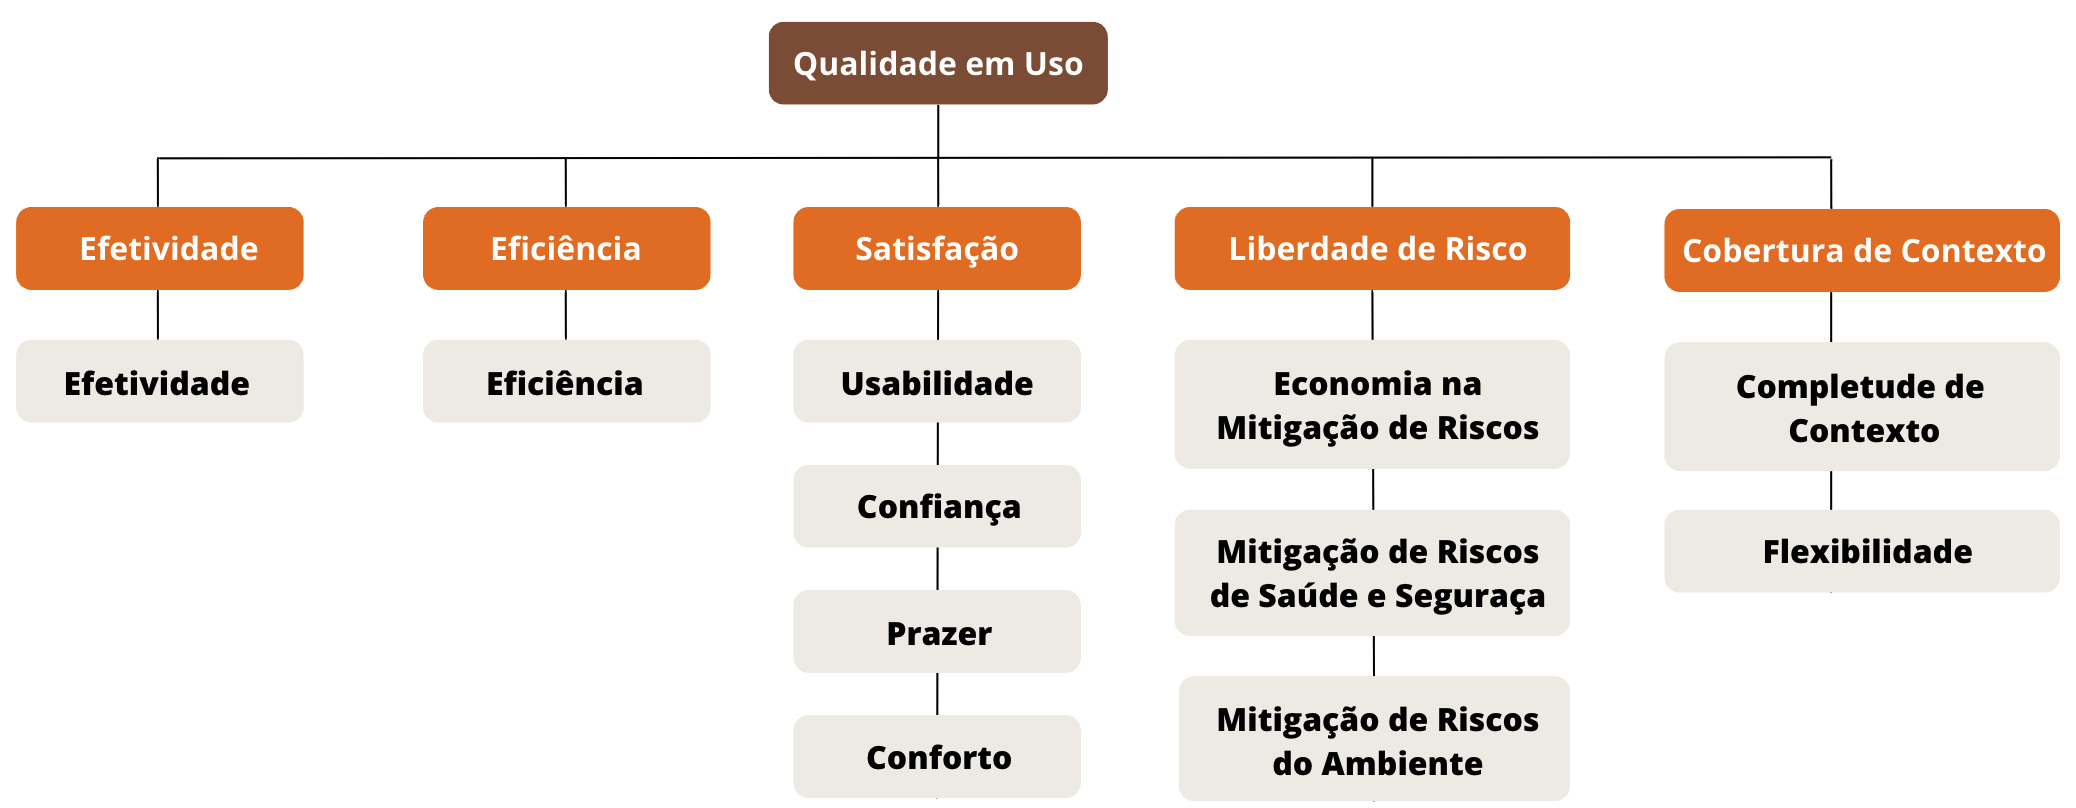
\includegraphics[width=1\linewidth]{figuras/quality_in_use.png}
% \text Fonte: Adaptado da Norma \citeonline{iso25010}
% \label{fig:model-quality-in-use}
% \end{figure}

\section{Problema}

Mesmo com o conhecimento de especialistas de negócio e de gerentes de produto, prever as necessidades do usuário é, na maioria das vezes, impreciso \cite{castellion2008do}. Além disso, a coleta direta de opiniões dos usuários também pode não ser assertiva, já que, aquilo que um usuário imagina que deseja muitas vezes difere do que ele realmente utilizaria na prática. Além disso, generalizar os resultados de uma análise qualitativa nem sempre é viável ou ideal \cite{cao2008agile}.

Considerando essa conjuntura, a análise quantitativa por meio de experimentos se apresenta como uma alternativa mais precisa, com a formalização de hipóteses e a definição de métricas-chave para observação \cite{kohavi_oce_and_ab_tests_2017}. No entanto, esse processo exige uma instrumentação adequada para garantir a confiabilidade estatística dos testes realizados. Para isso, é essencial uma definição sistemática do processo de desenvolvimento, incluindo a coleta e análise de dados.

A literatura apresenta diferentes modelos e técnicas para o desenvolvimento orientado a dados, porém carece de uma compreensão compartilhada sobre definições, processos e estratégias, o que dificulta a adoção da prática \cite{quin_b_2024}. Assim, \textbf{a falta de sistematização da coleta e da análise de dados torna a avaliação da qualidade em uso de um produto mais difícil e, muitas vezes, imprecisa}. Esse cenário faz com que a priorização do que será desenvolvido se baseie apenas em opiniões dos envolvidos na construção do produto, ao invés de um processo orientado à tomada de decisão baseada em dados \cite{olsson_opinions_2014}.

\section{Questão de Pesquisa} 
\label{sec:questao}

Para definir a questão de pesquisa norteadora deste trabalho foi utilizada a abordagem \textit{Goal Question Metric} (GQM), que propõe a especificação hierárquica de objetivos, questões e métricas de maneira \textit{top-down}, vide Figura \ref{fig:GOAL_QUESTION_METRIC}. O propósito desta abordagem é tornar o planejamento e a mensuração dos objetivos de uma pesquisa em questões e métricas que embasem suas respostas. Seguindo essa estrutura e a adaptando para o contexto desta pesquisa, definiram-se as seguintes características: propósito, foco, objeto de estudo e ponto de vista (vide Tabela \ref{tab:gqm}). Com isso, foi formulada a questão de pesquisa norteadora deste trabalho:

\begin{figure}[h] 
    \centering
    \caption{Estrutura do Modelo GQM}
    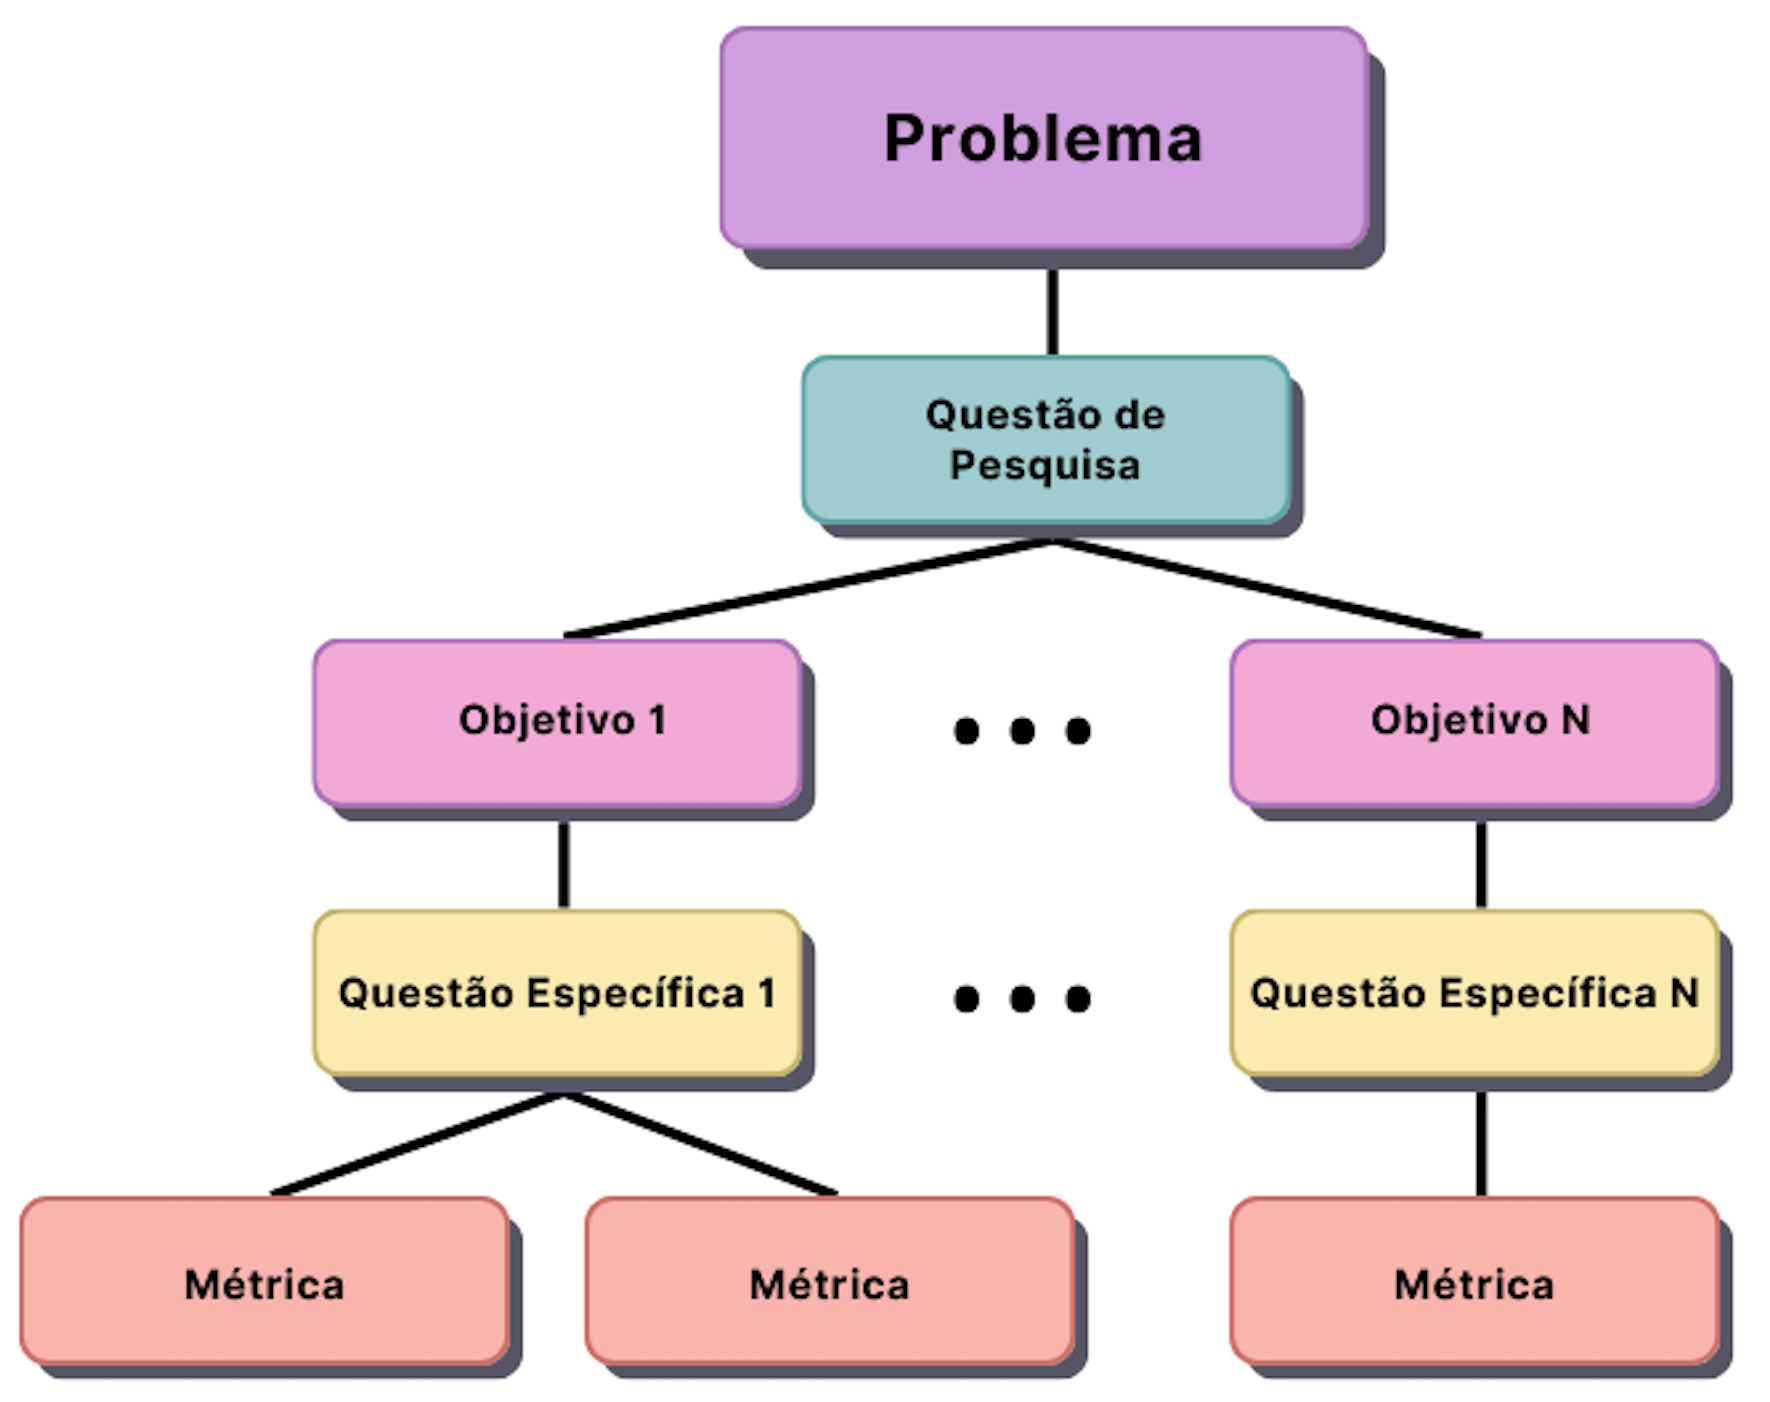
\includegraphics[width=0.75\textwidth]{figuras/gqm.png}

    \begin{center}
    \text Fonte: Adaptado de  \citeonline{basili_goal_1994}
    
    \end{center}
    \label{fig:GOAL_QUESTION_METRIC}
\end{figure}


\begin{table}[h!]
\centering
    \caption{Características de Definição da Questão de Pesquisa}
        \begin{tabular}{|p{4cm}|p{10cm}|}
            \hline
            \textbf{Característica} & \textbf{Valor} \\
            \hline
            Analisar & Versões de produto de \textit{software} \\
            Propósito & Avaliar \\
            Foco & Adoção de práticas de experimentação contínua para embasar a tomada de decisão na implantação de novas versões de um produto de \textit{software} \\
            Objeto de Estudo & Produto de \textit{Software} \\
            Ponto de Vista & Pesquisador \\
            Contexto & Manutenção e evolução de um produto de \textit{software}, em uma organização privada brasileira \\
            \hline
        \end{tabular}
   
 
    \begin{center}
        \text{Fonte: Adaptado de \citeonline{basili_goal_1994}}   
    \end{center}

    \label{tab:gqm}
\end{table}



\begin{center}
    \textit{Como a adoção de práticas de experimentação contínua pode auxiliar a tomada de decisão sobre a implantação de novas versões de um produto de software?}   
\end{center}



\section{Objetivos}
\label{subsec:objetivos-pesquisa}

O principal objetivo deste estudo é investigar como a adoção de práticas de experimentação contínua pode auxiliar na análise da qualidade em uso em um produto de \textit{software} e na tomada de decisão estratégica. Para alcançar esse objetivo geral, foram definidos os seguintes objetivos específicos, que deverão guiar a realização da primeira etapa deste trabalho:

\begin{itemize} 
    \item Realizar um levantamento teórico nas áreas de experimentação, qualidade de \textit{software}, análise estatística  de dados e desenvolvimento orientado a dados; 
    \item Adaptar o processo de desenvolvimento já existente no produto avaliado, incluindo práticas de experimentação contínua para posterior execução e avaliação; 
    \item Planejar um estudo de caso para observar a aplicação do processo proposto no ambiente real de desenvolvimento e uso do produto, objeto desta investigação;
    \item Executar as atividades propostas, coletar métricas de uso e comparar diferentes versões do produto de \textit{software}, avaliando estatisticamente qual delas foi melhor recebida pelos usuários. Ou seja, qual versão apresenta melhor atributo de qualidade em uso percebido. Além disso, documentar e analisar os resultados dos experimentos;
    \item Realizar uma coleta de opinião dos envolvidos no processo em relação às atividades realizadas; e 
    \item Analisar e documentar os principais achados deste estudo. 
\end{itemize}

% \section{Metodologia}

% \subsection{Classificação Metodológica}


% \begin{figure}[H]
% \centering
% \caption{Titulo da imagem}
% \includegraphics[width=1\textwidth]{figuras/secao-metodologia/Metodologia.png}
% \legend {Colocar aqui a legenda da figura}
% \label{fig:metodologia}
% \end{figure}

% \subsection{Plano Metodológico}
% Conforme Brereton et al (BRERETON et al., 2008), o processo de um estudo de
% caso possui quatro fases principais: Planejamento; Coleta de Dados; Análise de Dados; e
% Relatórios, que compõem o plano metodológico adotado neste trabalho:

% O plano metodológico é baseado em \citeonline{brereton_2008}, que apresenta um \textit{Protocolo de Estudo de Caso}, com vários itens a serem desenvolvidos, e esses distribuídos em quatro grandes fases: Planejamento; Coleta de Dados; Análise de Dados; e Relatórios.

% Essas fases compreendem, de forma resumida:

% \begin{itemize}
%     \item \textbf{Planejamento da Pesquisa:} nessa fase apresenta-se o contexto do pesquisa com a revisão bibliográfica, pergunta de pesquisa,  definição dos objetivos do trabalho e a definição de um plano metodológico, com as escolhas metodológicas;
    
%     \item \textbf{Coleta dos Dados:} essa fase compreende o levantamento e a aplicação das técnicas de coleta de dados como revisão documental, revisão bibliográfica e estudo de caso;
    
%     \item \textbf{Análise dos Dados:} nessa fase realizam-se a interpretação e análise dos dados coletados, assim como a análise da validade do trabalho, cuja meta é avaliar a percepção dos gestores da empresa em relação as diretrizes propostas;
    
%     \item \textbf{Relatório:} por fim, o relatório é constituído pelos resultados deste trabalho e caracterizado por esta monografia.
% \end{itemize}

% O planejamento metodológico do \textit{Protocolo de Estudo de Caso} \cite{brereton_2008} é apresentado no Capítulo Proposta (REVISAR - ALINHAR COM NOVA ESTRUTURA).



\section{Organização do Trabalho}
\label{sec:organizacao}

Esta subseção visa apresentar a estrutura do documento e o que está presente em cada capítulo desta monografia.

\begin{itemize}
    \item \textbf{Introdução:} apresentação do trabalho, do seu contexto e problemática, além da sua questão de pesquisa e objetivos;
    \item \textbf{Referencial Teórico:} fundamentação teórica do presente trabalho; explanação sobre os principais tópicos relacionados ao contexto desta pesquisa: experimentação em \textit{software}, qualidade de \textit{software}, experimentos controlados, análise de dados e experimentação contínua;
    \item \textbf{Revisão Estruturada da Literatura:} metodologia empregada para a seleção dos estudos que compõem o material bibliográfico; descrição do protocolo utilizado para busca e seleção dos artigos, bem como os resultados desta pesquisa;
    \item \textbf{Proposta de Estudo de Caso:} descrição da estratégia de pesquisa e seu protocolo; definição dos objetivos e da questão de pesquisa; definição e apresentação das atividades a serem realizadas na segunda parte desta monografia; e
    \item \textbf{Condições do Trabalho:} visão geral sobre a situação atual desta investigação; apresentação das atividades já concluídas e daquelas que serão realizadas na segunda etapa desta monografia.
\end{itemize}


\section{Cronograma e Fluxo de Atividades}\label{cronograma}

\subsection{Atividades da Primeira Etapa}
\label{cronograma1}

Esta subseção visa discriminar as atividades realizadas na primeira etapa do trabalho, os apresentando também em forma de fluxo na Figura \ref{fig:atividades_1} e às dispondo cronologicamente na Figura \ref{fig:cronograma_1}.

\begin{itemize}
    \item \textbf{Contextualização em Experimentação na Engenharia de Software:} leituras com o intuito de compreender o processo de experimentação e a abordagem científica necessária para a realização da Revisão da Literatura da primeira parte desta pesquisa, bem como do Estudo de Caso e do Experimento que serão realizados na segunda parte;
    \item \textbf{Contextualização em Experimentação Contínua:} leitura de materiais referentes ao processo de Experimentação Contínua e Desenvolvimento Orientado a Dados com o objetivo de compreender o estado da arte, identificar as lacunas existentes e moldar os objetivos deste trabalho; consumo de materiais para capacitação do pesquisador nas áreas de qualidade de software e experimentos científicos;
    \item \textbf{Definição dos Objetivos e Protocolo de Pesquisa:} definição do protocolo de revisão da literatura e dos objetivos da pesquisa segundo a abordagem GQM \cite{basili_goal_1994}, além dos objetivos específicos e da questão de pesquisa do trabalho; formulação do protocolo de pesquisa conforme proposto por \citeonline{kitchenham_rsl}: questões de pesquisa da revisão, \textit{string} de busca, critérios de inclusão e exclusão e formulário de extração de dados;
    \item \textbf{Busca e Seleção dos Artigos:} execução da \textit{string} de busca e seleção do primeiro grupo de artigos a partir da leitura de título e resumo; processo de \textit{snowballing} a partir dos artigos selecionados, selecionando novos materiais a partir da leitura parcial dos mesmos (título e resumo e, caso necessário, introdução e conclusão);
    \item \textbf{Leitura do Material Selecionado:} leitura integral do material selecionado com o objetivo de compreender o estado da arte, conhecer os modelos e processos já existentes e construir o corpo de conhecimento necessário para a formulação da proposta de estudo de caso;
    \item \textbf{Definição da Proposta de Processo:} elaboração da proposta de processo de experimentação; formalização da proposta de estudo de caso, discriminando objetivos, objeto, instrumentalização e atividades a serem realizadas;
    \item \textbf{Escrita do Trabalho:} redação da monografia seguindo a organização apresentada na Seção \ref{sec:organizacao};
    \item \textbf{Revisão da Monografia:} revisão e correção; e
    \item \textbf{Apresentação do Trabalho:} apresentação da primeira parte desta monografia para a banca avaliadora.
\end{itemize}

\begin{figure}
    \caption{Fluxo de Atividades Realizadas na Primeira Etapa Desta Monografia}
    \centering
    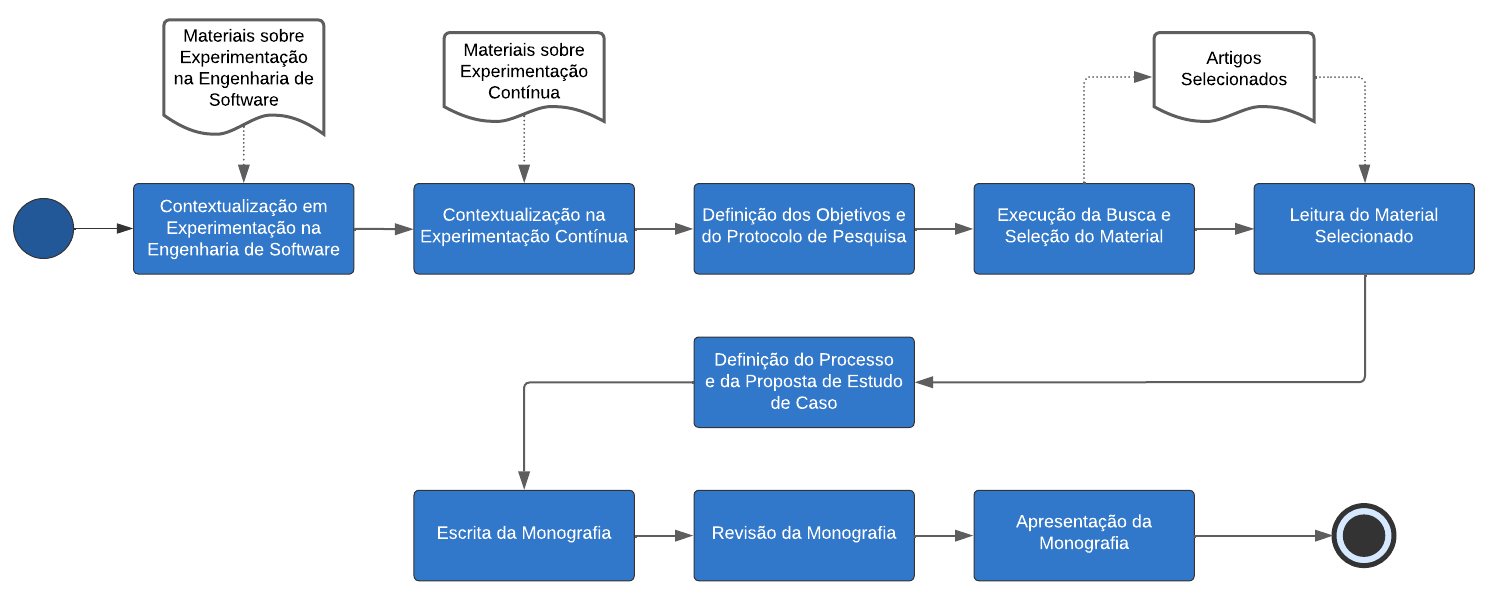
\includegraphics[width=1\linewidth]{figuras/atividades1.png}
    \text{Fonte: Autor}
    \label{fig:atividades_1}
\end{figure}

\begin{figure}
    \caption{Cronograma Realizado na Primeira Etapa da Monografia}
    \centering
    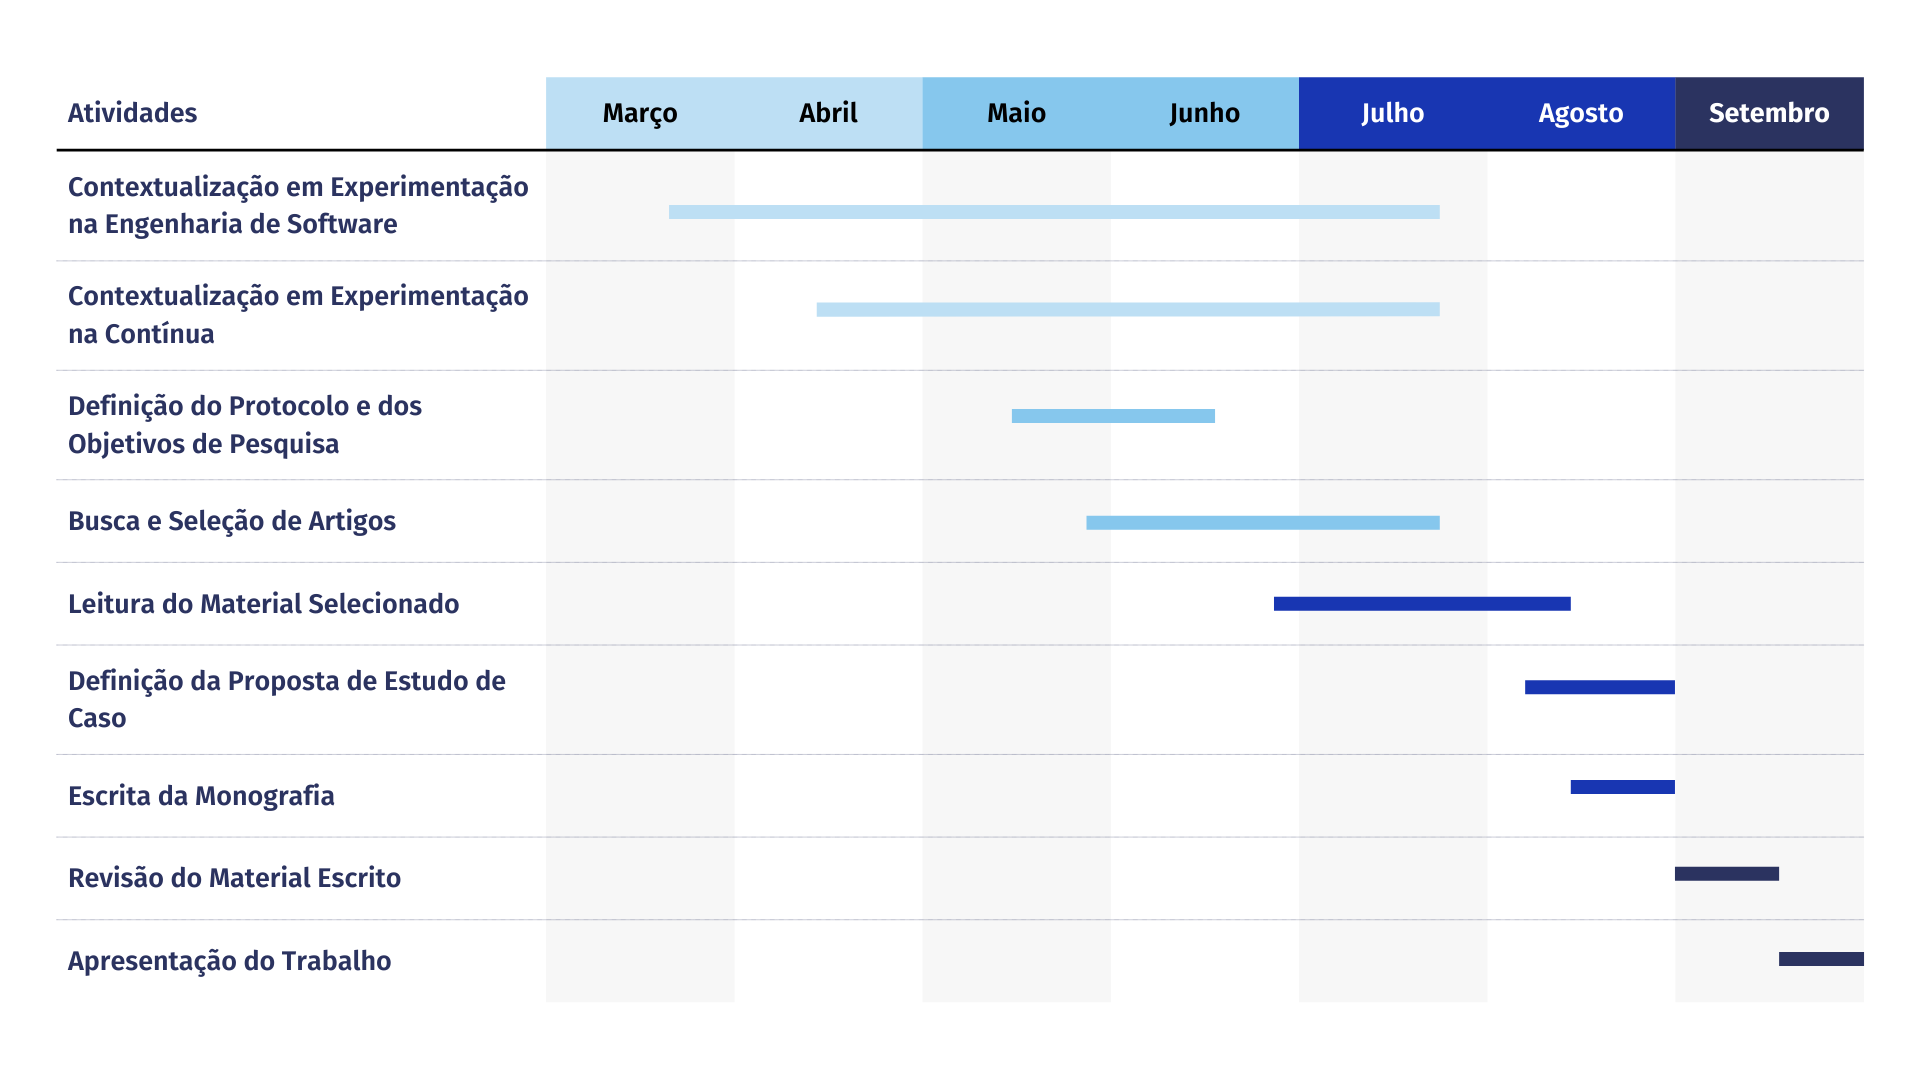
\includegraphics[width=1\linewidth]{figuras/cronograma1.png}
    \text{Fonte: Autor}
    \label{fig:cronograma_1}
\end{figure}


\subsection{Atividades da Segunda Etapa}
\label{cronograma2}

Esta subseção visa apresentar as atividades planejadas para a segunda etapa deste trabalho,
as apresentando em forma de fluxo na Figura \ref{fig:atividades_2} e as dispondo em forma de cronograma na Figura \ref{fig:cronograma_2}.

\begin{itemize}
    \item \textbf{Evolução do Trabalho:} revisão e atualização do material já escrito a partir das considerações da banca avaliadora;
    \item \textbf{Formulação de Hipóteses:} realização das atividades referentes à Engenharia de Hipóteses; geração, documentação e priorização de hipóteses para escolher aquela que será desenvolvida e observada através da execução do experimento objeto do Estudo de Caso deste trabalho;
    \item \textbf{Instrumentação do Experimento:} prototipação da hipótese selecionada; definição das métricas escolhidas para validação da hipótese; preparo dos disparos de evento para coleta dos dados; validação do \textit{design do experimento}; revisão da hipótese ou das métricas elencadas, caso necessário;
    \item \textbf{Desenvolvimento e Coleta de Dados:} desenvolvimento da nova versão de software (tratamento) a ser comparada com a versão já existente (controle); liberação da nova versão para os usuários beta a fim de iniciar a iteração do experimento (a coleta de dados já deve acontecer a partir desta liberação);
    \item \textbf{Análise de Dados:} iteração no experimento caso necessário (como, por exemplo, dados coletados insuficientes, necessidade de prolongamento do experimento); análise dos dados coletados para os testes de hipótese; decisão sobre a liberação da versão de tratamento para todos os usuários ou abandono da mesma;
    \item \textbf{Documentação do Resultado do Experimento:} documentação dos resultados do teste da hipótese para registro e criação de um corpo de conhecimento que auxilie futuros experimentos;
    \item \textbf{Coleta de Percepção dos Envolvidos:} pesquisa de opinião com os colaboradores envolvidos no estudo de caso para avaliação do processo proposto;
    \item \textbf{Análise dos Resultados do Estudo de Caso:} resposta às questões de pesquisa do estudo de caso a partir dos dados coletados, com posterior resposta à principal questão de pesquisa; descrição do processo realizado e documentação dos resultados obtidos;
    \item \textbf{Revisão da Monografia:} revisão e correção minuciosa do trabalho em busca de possíveis correções ou atualizações necessárias, tanto por parte do pesquisador quanto do orientador; e
    \item \textbf{Apresentação do Trabalho Finalizado:} apresentação da monografia finalizada à banca avaliadora.
\end{itemize}

\begin{figure}
    \caption{Fluxo de Atividades Planejadas Para a Segunda Etapa da Monografia}
    \centering
    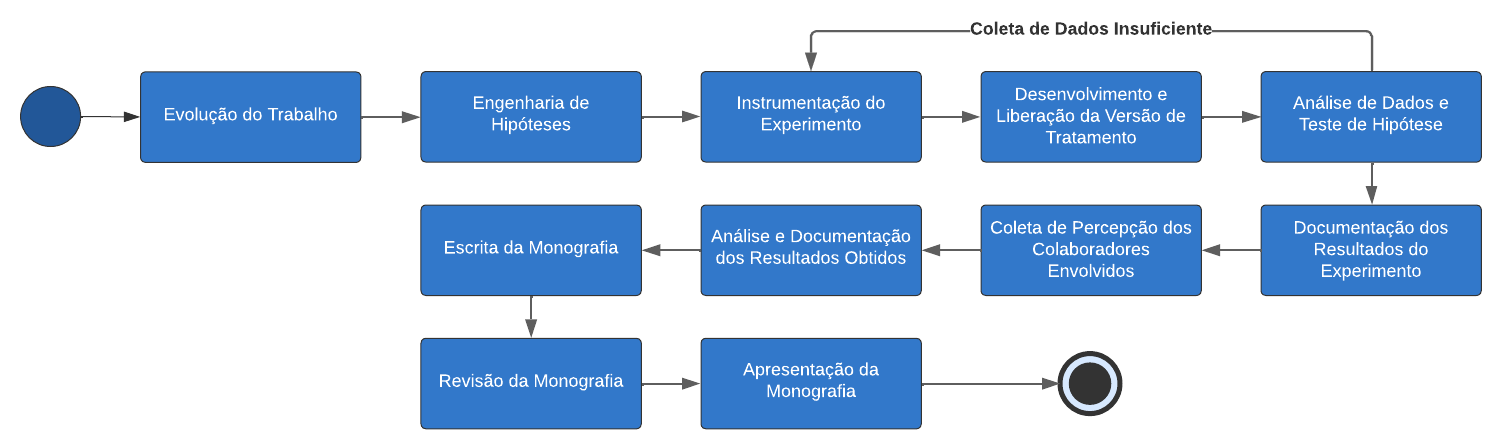
\includegraphics[width=1\linewidth]{figuras/atividades2.png}
    \text{Fonte: Autor}
    \label{fig:atividades_2}
\end{figure}
\begin{figure}
    \caption{Cronograma Planejado Para a Segunda Etapa da Monografia}
    \centering
    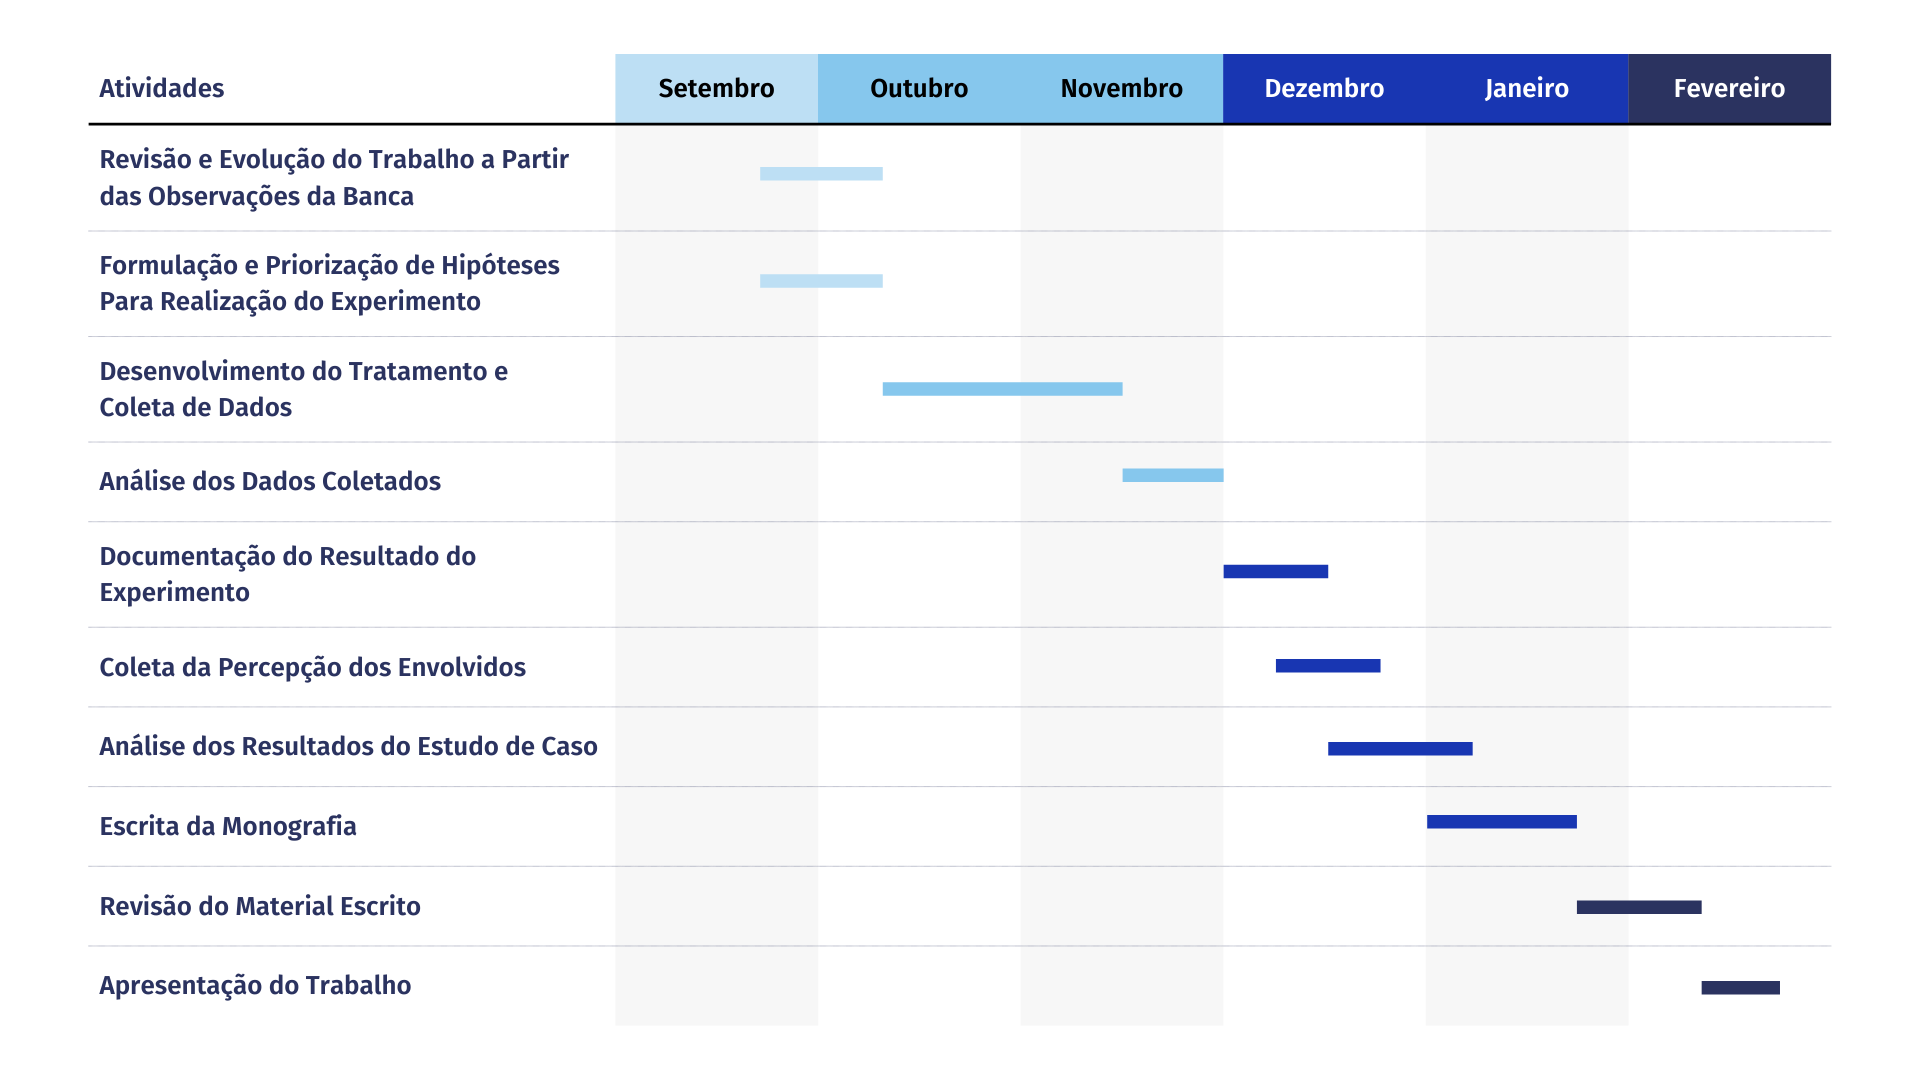
\includegraphics[width=1\linewidth]{figuras/cronograma2.png}
    \text{Fonte: Autor}
    \label{fig:cronograma_2}
\end{figure}

\chapter{Referencial Teórico}
\label{ch:referencial}

Neste capítulo é apresentada a fundamentação teórica deste trabalho, abordando conceitos e metodologias e facilitando a compreensão das tomadas de decisão que construíram a proposta de estudo apresentada no Capítulo \ref{ch:proposta}.

\section{Experimentação na Engenharia de Software}
\label{subsec:experimentacao}

A experimentação é um domínio fundamental da investigação empírica, oferecendo uma abordagem disciplinada e quantificável para a análise de fenômenos de interesse. Na engenharia de software, essa abordagem é crucial, pois trata-se de uma área multidisciplinar que depende diretamente da avaliação da atividade humana. A pesquisa científica se torna especialmente relevante em momentos de tomada de decisão sobre como softwares são desenvolvidos, contribuindo para o avanço do conhecimento por meio da avaliação das atividades realizadas por pessoas em seus diferentes contextos \cite{wohlin_experimentation_2012}.

\citeonline{basili_experimental_1993} apresentou quatro métodos de pesquisa na Engenharia de \textit{Software}: \textit{Scientific}, \textit{Engineering}, \textit{Empirical} e \textit{Analytical}. Dentre eles, o método Empírico (\textit{Empirical}) é amplamente utilizado em ciências sociais e psicologia para estudar o comportamento humano em contextos onde leis formais não se aplicam, sendo igualmente aplicável à Engenharia de \textit{Software} quando se é necessário lidar com aspectos que não são puramente técnicos \cite{wohlin_experimentation_2012}.

Entre as estratégias de investigação empírica está o \textbf{Estudo de Caso}, que utiliza diversas fontes de dados para investigar um fenômeno em seu contexto real. Este método avalia o caso em questão de forma quantitativa ou qualitativa, sem intervenção ou controle, sendo, portanto, um estudo observacional \cite{runeson_case_study_2012}.

Outra estratégia é o \textbf{Experimento}, que, ao contrário do estudo de caso, busca um controle sistemático e direto sobre a situação estudada. Para isto, identifica o contexto de interesse e coleta amostras de variáveis para validar teorias, confirmar ou explorar relacionamentos. É normalmente utilizado quando o objetivo é comparar diferentes tratamentos para uma mesma situação \cite{wohlin_experimentation_2012}.

Utilizada no contexto deste trabalho, há também a \textbf{Revisão Sistemática da Literatura}, que busca reunir evidências empíricas de diversas fontes literárias através de buscas em portais, bancos de dados acadêmicos ou outras fontes. Dessa forma, através do seu protocolo, é possível sintetizar o estado da arte do domínio desejado por meio de uma avaliação sistemática das informações encontradas na literatura \cite{kitchenham_rsl}.

\todo[inline, color=pink]{Salvo engano eu havia feito um comentário nesse semtido. Essa introdução ficou restrita. Por mais que você detalhe os métodos que você vai utilizar, nessa introdução, precisa apararecer uma visão geral. Tipo o cap.2  do Wohlin. Por exemplo, flatou falar de survey/questionário, pesquisa-ação, estudos etnográficos...}


\subsection{Experimento}

Este método de investigação permite a exploração e validação de relacionamentos através de testes de hipótese e análises estatísticas. Seguindo o apresentado por \citeonline{wohlin_experimentation_2012}, serão apresentados os principais artefatos envolvidos neste processo, bem como as etapas necessárias para sua realização.

\subsubsection{Artefatos}

\begin{itemize}
    \item \textbf{Variáveis}: ao conduzir um experimento, se observa o comportamento de determinadas variáveis durante o processo escolhido. Aquelas que são alteradas para gerar os resultados são chamadas de \textbf{variáveis independentes}, ou \textbf{fatores}. Já aquelas que são responsáveis por informar os efeitos encontrados, são as \textbf{variáveis dependentes};
    \item \textbf{Tratamentos}: valor particular e específico aplicado a um fator. Cada tratamento representa uma configuração particular que é testada no experimento;
    \item \textbf{Objetos}: são os elementos ou itens sobre os quais os tratamentos são aplicados e avaliados, ou seja, quaisquer artefatos ou processos que estejam sendo estudados ou testados, e
    \item \textbf{Sujeitos}: participantes do experimento. Aqueles que são expostos aos diferentes tratamentos.
\end{itemize}

\subsubsection{Processo}

\begin{itemize}
    \item \textbf{Definição de Escopo:} onde se define claramente o problema, os objetivos e as metas do estudo. É crucial estabelecer o escopo para direcionar adequadamente o experimento, o que inclui a formulação inicial da hipótese, a definição do objeto de estudo, o propósito, o foco de qualidade, a perspectiva e o seu contexto;
    \item \textbf{Planejamento:} nesta fase são elaborados os detalhes necessários para a execução do estudo. A hipótese a ser testada é formalizada, são indetificadas as variáveis independentes e dependentes, escolhe-se o \textit{design} do experimento e são preparados os instrumentos necessários. É importante determinar os valores das variáveis e preparar os objetos de estudo, assim como desenvolver diretrizes para a coleta de dados e avaliar a validade dos resultados esperados;
    \item \textbf{Operação:} condução efetiva do experimento. Esta fase inclui a preparação dos sujeitos e materiais, a execução do experimento conforme o planejamento e a validação dos dados coletados para garantir que são corretos e representativos. A execução deve seguir o plano estabelecido para assegurar a integridade dos resultados;
    \item \textbf{Análise e Interpretação:} envolve analisar e interpretar os dados coletados. Utiliza-se estatísticas descritivas para compreender os dados e realiza-se testes de hipótese para avaliar a relação entre as variáveis. A análise pode incluir a redução de dados e a interpretação dos resultados, ajudando a validar as conclusões do experimento;
    \item \textbf{Apresentação e Empacotamento:} concentra-se na documentação e apresentação dos resultados do experimento. O objetivo é comunicar os achados de forma clara e eficaz, o que pode incluir a preparação de relatórios, a publicação dos resultados e a criação de pacotes de laboratório para facilitar a replicação do estudo. Uma documentação completa e detalhada é essencial para garantir que os resultados possam ser replicados e utilizados para futuras pesquisas.
\end{itemize}


\subsection{Estudo de Caso}

Permite uma compreensão aprofundada e contextualizada dos fenômenos de interesse através de investigações dentro de seus contextos reais. Além disso, é flexível, o que possibilita ajustes iterativos em diferentes momentos do processo. A seguir, serão definidas suas etapas de realização: definição, preparação e coleta de dados, análise de dados e relato dos resultados \cite{yin_case_study_2009}.

\subsubsection{Definição}

Segundo \citeonline{wohlin_experimentation_2012}, é a etapa inicial, nela são definidas as bases da pesquisa, através do levantamento dos seguintes artefatos:

\begin{itemize}
    \item \textbf{Objetivo:} inicialmente, é formulado de forma genérica, com um foco principal que será refinado ao longo do estudo. Define o que o pesquisador pretende alcançar e as perguntas que guiarão a investigação;
    \item \textbf{Caso:} definição do objeto de estudo da pesquisa. Pode ser um projeto, um processo, um grupo de pessoas, ou qualquer outro fenômeno que esteja sendo investigado. O caso deve necessariamente ser observado em seu contexto real, permitindo que o pesquisador capture as complexidades e nuances do ambiente;
    \item \textbf{Trabalhos Relacionados:} resultado de uma revisão sobre o estado geral da área de conhecimento à ser estudada, visando pontos de partida em outros trabalhos. Ajuda a identificar lacunas de pesquisa, construir o referencial teórico e fornecer embasamento para a formulação das questões de pesquisa;
    \item \textbf{Questões de Pesquisa:} devem ser claras e orientadoras. Funcionam como um norte para o estudo, direcionando o processo de coleta e análise de dados. Perguntas bem formuladas garantem que o estudo permaneça focado e relevante, abordando as principais preocupações do fenômeno em análise;
    \item \textbf{Métodos:} abordagem de coletas de dados à serem adotadas, dependem das questões de pesquisa e do contexto. A definição clara dos métodos contribui para a validade e confiabilidade do estudo. E
    \item \textbf{Seleção:} refere-se à escolha das fontes de dados e dos participantes do estudo. É crucial que essas escolhas sejam feitas de maneira consciente, considerando a relevância e representatividade das fontes em relação ao objetivo do estudo.
\end{itemize}

\subsubsection{Preparação e Coleta de Dados}
Aqui, o pesquisador deve estruturar cuidadosamente o processo, garantindo que os dados coletados sejam pertinentes e válidos. \citeonline{wohlin_experimentation_2012} destacam a importância da triangulação, que envolve o uso de múltiplas fontes de dados para fortalecer a validade dos resultados. 

A coleta de dados é uma etapa crítica e pode ocorrer de maneira contínua ao longo do estudo. A combinação de diferentes métodos e fontes de dados fortalece a pesquisa e proporciona uma visão mais abrangente do fenômeno. De acordo com \citeonline{lethbridge2005studying},  as técnicas de coleta de dados são divididas em três graus:

\begin{itemize}
    \item \textbf{Primeiro Grau:} técnicas que exigem contato direto com os participantes, como entrevistas, questionários e grupos de discussão. Essas técnicas fornecem dados ricos e detalhados, mas exigem maior envolvimento do pesquisador e podem ser mais caras e demoradas.
    
    \item \textbf{Segundo Grau:} envolve a observação direta do ambiente de estudo sem interação com os participantes. Exemplos incluem a observação do trabalho de uma equipe ou a coleta de métricas de um sistema em funcionamento. Essas técnicas permitem captar o comportamento natural dos participantes, mas podem ser limitadas em termos de profundidade.
    
    \item \textbf{Terceiro Grau:} utiliza dados já existentes, como documentação e registros históricos. Embora menos intrusivos, esses métodos podem ser limitados pela qualidade e relevância dos dados disponíveis. No entanto, são úteis para complementar as técnicas de primeiro e segundo grau.
\end{itemize}

\subsubsection{Análise de Dados}

Processo de interpretação e  busca de padrões nos dados coletados, e que permite ao pesquisador identificar as relações entre as variáveis e os resultados observados \cite{yin_case_study_2009}. Segundo \citeonline{wohlin_experimentation_2012}, a análise de dados pode ser realizada por meio de técnicas qualitativas, quantitativas ou uma combinação de ambas, dependendo da natureza dos dados e dos objetivos da pesquisa.

Para garantir uma análise robusta, \citeonline{wohlin_experimentation_2012} sugerem a adoção de estratégias de categorização dos dados, onde os dados são organizados em categorias ou temas, facilitando a identificação de padrões e a construção de teorias baseadas nas evidências empíricas. O uso de software de análise qualitativa pode ser útil para codificar e categorizar grandes volumes de dados textuais.

Além disso, a análise de dados pode incluir a verificação de validade interna e a validação cruzada dos resultados, assegurando que as conclusões não sejam apenas fruto de coincidências ou de vieses do pesquisador, mas que realmente representem o fenômeno estudado \cite{yin_case_study_2009}.

\subsubsection{Relato}

\citeonline{robson2002real} destaca que o relato é essencial não apenas para comunicar os resultados da pesquisa, mas também para permitir a avaliação da qualidade do estudo por parte de outros pesquisadores, e que, para isto, deve abordar os seguintes aspectos:

\begin{itemize}
\item \textbf{Contexto:} Descrição detalhada do ambiente em que o estudo foi conduzido, incluindo informações sobre os participantes, o período e as condições específicas que podem ter influenciado os resultados. Essa seção deve permitir ao leitor compreender as particularidades do caso estudado, ajudando a contextualizar os resultados.

\item \textbf{Procedimentos:} Explicação das etapas seguidas ao longo do estudo, desde a definição do caso até a coleta e análise dos dados. A clareza na descrição dos procedimentos garante a transparência metodológica, permitindo que outros pesquisadores avaliem a robustez do estudo e, eventualmente, o repliquem.

\item \textbf{Resultados:} Apresentação dos achados de forma estruturada, utilizando ferramentas como tabelas, gráficos e citações diretas dos participantes, quando aplicável, para ilustrar os pontos principais. Deve-se fornecer "instantâneos" relevantes dos dados coletados que sustentem as conclusões apresentadas, garantindo uma cadeia de evidências sólida.

\item \textbf{Discussão:} Interpretação dos resultados à luz da literatura existente, identificando as contribuições do estudo, suas limitações e as implicações práticas ou teóricas. A discussão deve situar os achados no contexto mais amplo do campo de estudo, explorando como eles se relacionam com pesquisas anteriores e quais novas questões surgem a partir das descobertas.

\item \textbf{Conclusões:} Resumo das principais descobertas e sugestões para pesquisas futuras. As conclusões devem sintetizar as contribuições do estudo e indicar como ele avança o conhecimento na área, além de propor direções para estudos subsequentes.
\end{itemize}

 
\section{\textit{Lean Startup}}

Esta metodologia \cite{ries2011lean} propõe uma abordagem contínua e sistemática de inovação sob a perspectiva das \textit{startups}, seu pensamento pode ser resumido em sete princípios: otimizar o todo, eliminar desperdícios, entregar valor, aprender constantemente, entregar rapidamente, engajar todos os participantes e melhorar continuamente \cite{poppendieck2003lean}. 


Para isso, o autor propõe um ciclo de aprendizado contínuo chamado \textit{Build-Measure-Learn}, para melhor compreensão dos desejos e das necessidades dos clientes. A fase de \textit{Build} foca na construção da funcionalidade, enquanto a fase de \textit{Measure} concentra-se na instrumentação dos dados de comportamento do usuário no sistema. Por fim, a fase de \textit{Learning} tem como objetivo usar os dados coletados para entender como as hipóteses e suposições foram realmente recebidas após a \textit{release}, a fim de construir um corpo de conhecimento sobre o produto e fomentar um ambiente de contínua inovação.

\section{\textit{Online Controlled Experiment}}

Também conhecido como Teste A/B ou simplesmente \textit{OCE}, é um experimento realizado no contexto \textit{online}. Esse tipo de investigação tem como objetivo analisar diferentes versões de \textit{software}, escolhendo métricas para comparar variantes de uma mesma funcionalidade e validar ideias sobre o desenvolvimento do produto (e.g., dispor os elementos de maneira diferente em uma página \textit{web} deve tornar determinada atividade mais rápida). A versão inicial, sem mudanças, é chamada de controle, e a atualizada, de tratamento \cite{fabijan_online_2020}.

Durante a utilização, os usuários são distribuídos entre essas diferentes versões, e, à medida que interagem com o produto, suas atividades são registradas e as métricas escolhidas são coletadas. A diferença entre esses valores, caso seja estatisticamente significativa e se a coleta de dados foi feita corretamente, muito provavelmente foi introduzida pelo tratamento \cite{kohavi_oce_and_ab_tests_2017}. Dessa forma, finaliza-se um fluxo contínuo de aprendizado, semelhante ao ciclo proposto pela metodologia \textit{Lean}. Esse ciclo já foi formalizado anteriormente na literatura e é apresentado na Figura \ref{fig:oce_lifecycle}.

\begin{figure}
    \centering
    \caption{\textit{The Experiment Lifecycle} }
    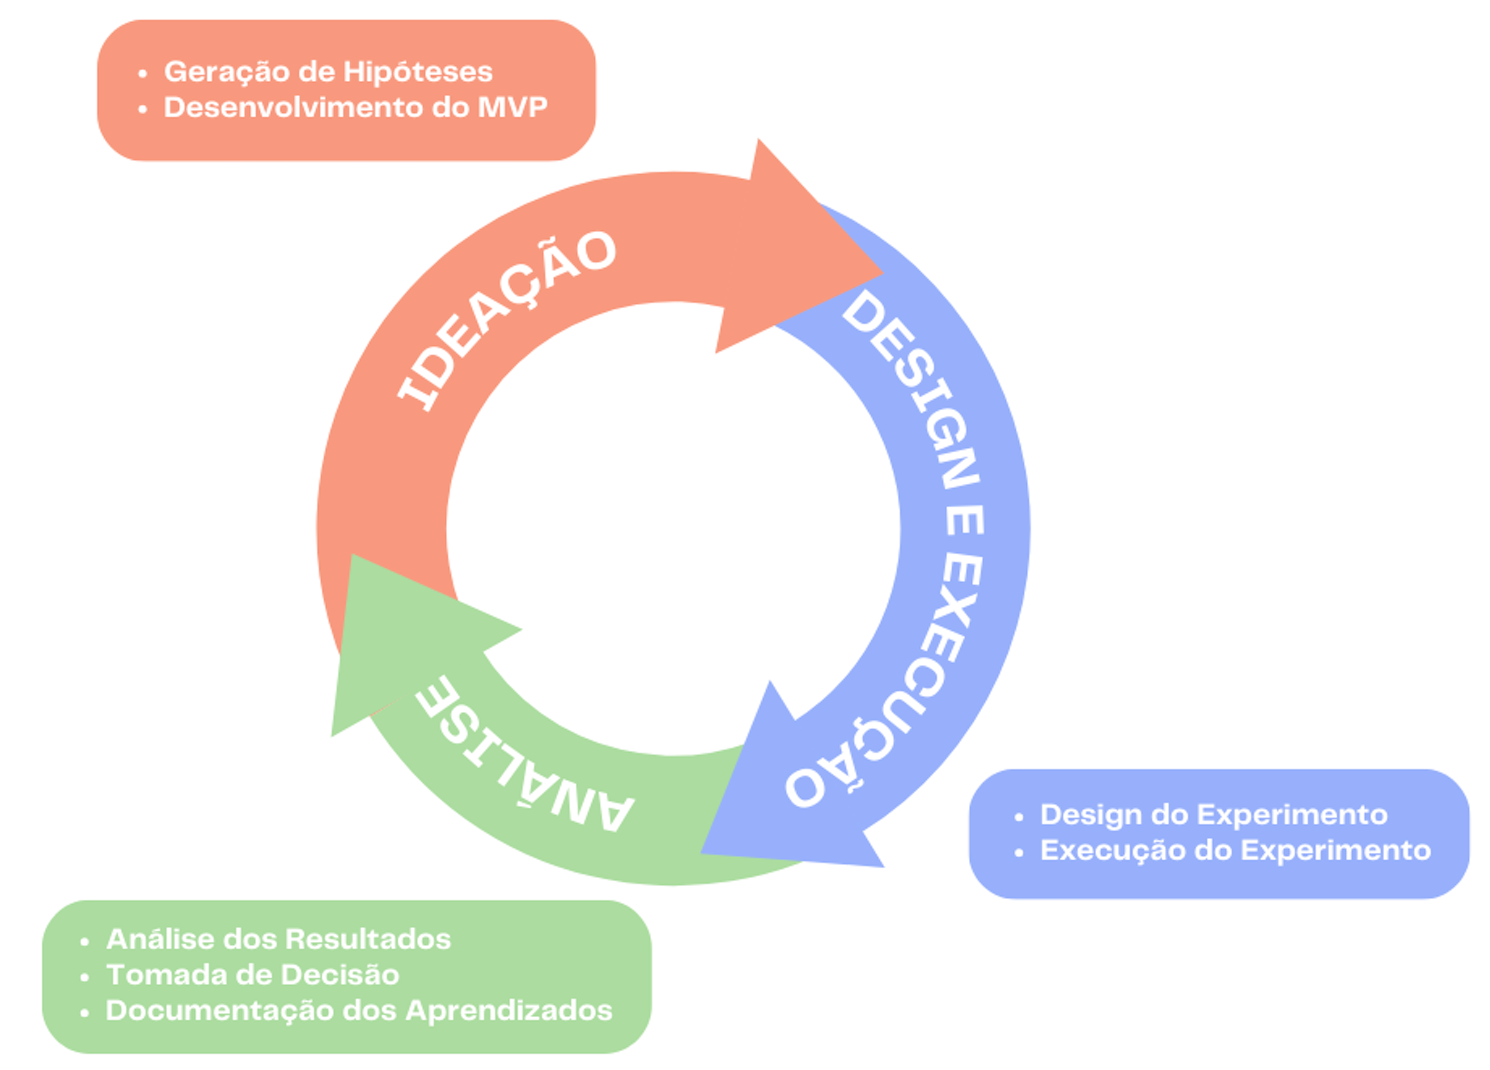
\includegraphics[width=0.75\linewidth]{figuras/oce_lifecycle.png}
    \text{Fonte: Adaptado de \citeonline{kohavi_online_2013}}
    \label{fig:oce_lifecycle}
\end{figure}

\section{\textit{Feature Toggles}}
\label{sec:ref-feature-toggle}

Nos últimos anos, empresas de \textit{software} têm priorizado cada vez mais a entrega contínua de funcionalidades para os seus usuários, diminuindo o tempo entre \textit{releases} \cite{humble_farley_2010}. Com isso, o processo de integração se torna mais complexo, já que é necessário unir diferentes entregas de diversas equipes de desenvolvedores a fim de gerar uma nova versão funcional e estável do produto \cite{berczuk_appleton_2002}.

Por ser um processo complicado, diversas soluções já surgiram no mercado; uma delas é a arquitetura de \textit{Feature Toggles} (também conhecidos como \textit{feature gates} ou \textit{feature flags}). Esta solução é um conceito simples: variáveis condicionais que envolvem determinados blocos de código, podendo ser habilitadas ou desabilitadas dependendo do contexto (por exemplo, ativar apenas para testes internos ou usuários beta). Essa abordagem em aplicações modernas permite que funcionalidades sejam ligadas ou desligadas em tempo de execução no lado do cliente, sem a necessidade de uma nova compilação \cite{rahman_feature_toggle_2016}.

Uma das desvantagens da utilização dessas \textit{flags} é a dívida técnica que elas geram, já que, uma vez que a funcionalidade tenha sido testada e liberada para a base total de usuários, a parte remanescente do código se torna obsoleta e inutilizada \cite{rahman_feature_toggle_2016}. Apesar disso, por viabilizar a divisão dos usuários entre versões diferentes de funcionalidades, esta arquitetura se mostra uma possível maneira de realizar experimentos e já é uma prática utilizada no mercado \cite{issa_mattos_hurrier_2023}.

\section{Qualidade de Software}

A qualidade do \textit{software} é um aspecto fundamental que impacta diretamente a eficácia do sistema em seu contexto de uso \citeonline{iso25000}. A norma \citeonline{iso25000} define a qualidade do produto de \textit{software} em termos de características e subcaracterísticas que determinam sua capacidade de satisfazer as necessidades explícitas e implícitas dos usuários. Além disso, a qualidade em uso refere-se ao efeito percebido pelo usuário final ao interagir com o \textit{software} em seu ambiente operacional.

A avaliação da qualidade de um produto de \textit{software} em uso é essencial para garantir que o sistema não apenas funcione conforme especificado, mas também atenda às expectativas e requisitos dos usuários em situações reais de operação. As características e subcaracterísticas da qualidade em uso são definidas pela norma \citeonline{iso25010} e são apresentadas na Figura \ref{fig:quality-in-use}.

\begin{figure}[h]
\centering
\caption{Modelo de Qualidade em Uso}
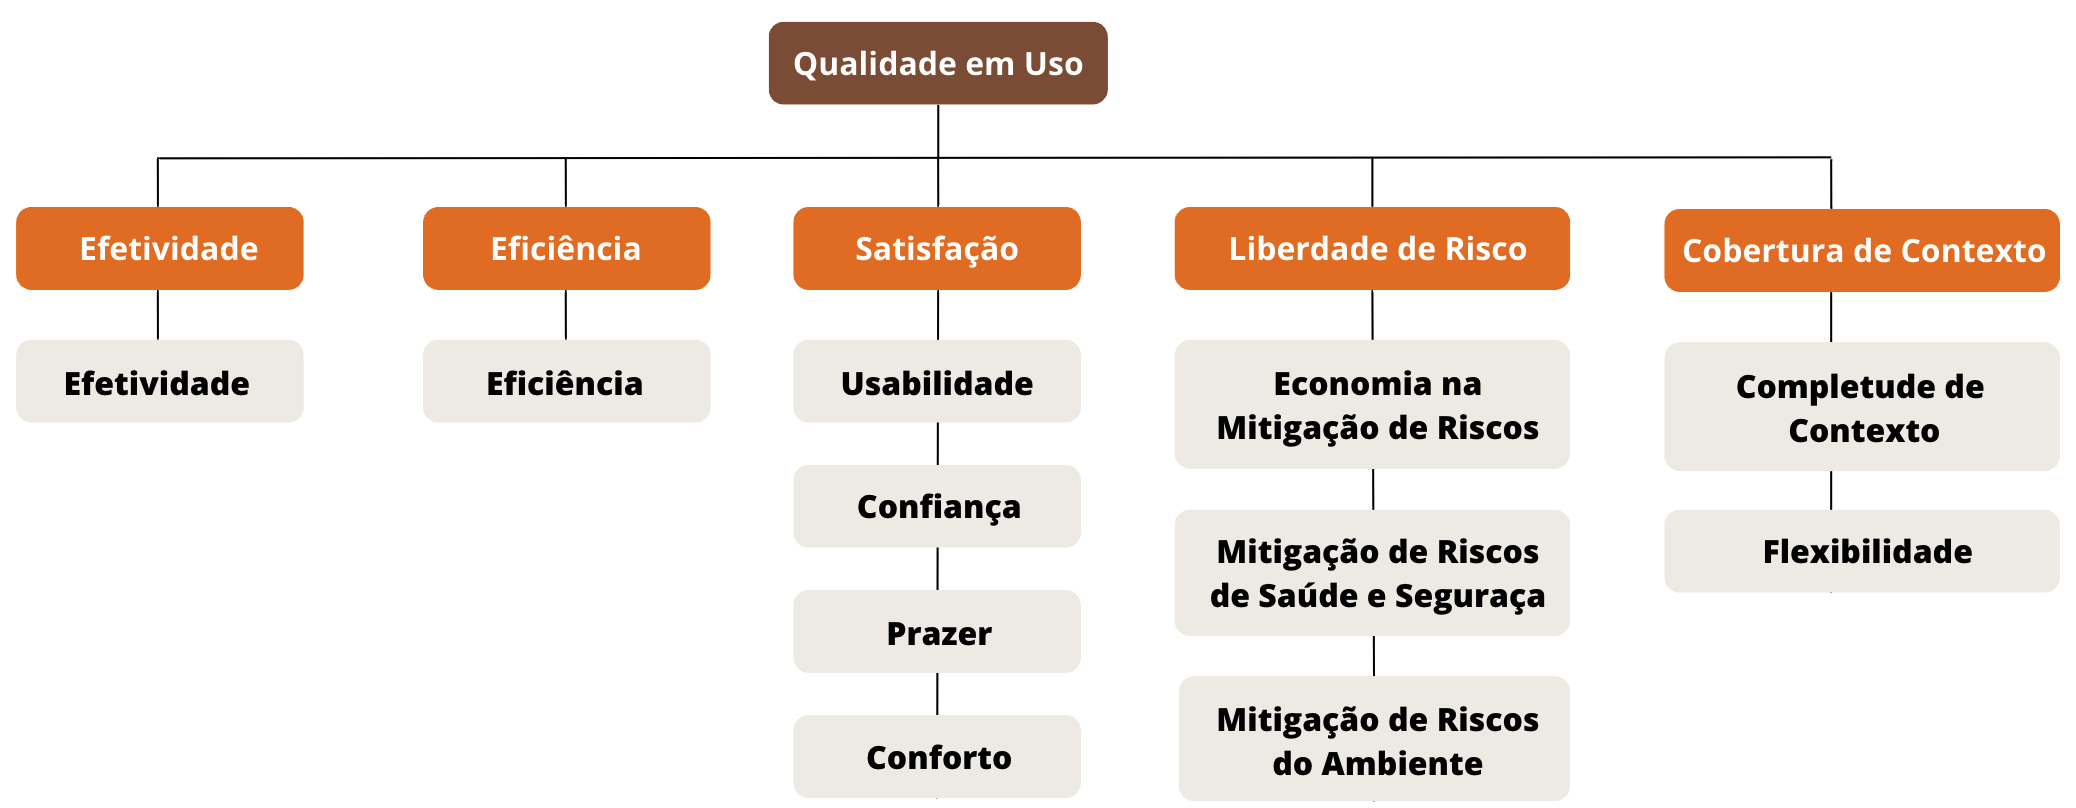
\includegraphics[width=1\linewidth]{figuras/quality_in_use.png}
\text{Fonte: Norma \citeonline{iso25010}}
\label{fig:quality-in-use}
\end{figure}

O foco desta monografia está na característica de qualidade de \textbf{eficácia}. A eficácia refere-se à precisão e à completude com que o \textit{software} permite que os usuários alcancem os objetivos esperados. A norma \citeonline{iso9241} define que, para avaliar determinada característica, devem ser definidas medidas de critério para tal, e exemplifica que, em termos de eficácia, estas devem estar relacionadas a quantidade de vezes que uma tarefa é realizada com sucesso, garantindo que o usuário alcançou seus objetivos específicos.

Os experimentos controlados visam, dentre outros objetivos, aumentar a qualidade do \textit{software}, entregando apenas as funcionalidades que realmente agregam valor para o usuário \cite{fabijan_online_2020}. As métricas observadas no momento de avaliar o tratamento em um experimento são escolhidas para validar se os usuários realmente preferem a nova versão, o que pode ser interpretado como nível de eficácia da variante.

\section{Experimentação Contínua}
\label{sec:ref-experimentacao-continua}

Na literatura, a Experimentação Contínua (ou \textit{Continuous Experimentation}, \textit{CE}) recebe diferentes denominações, como desenvolvimento orientado a dados (\textit{Data-Driven Development}), sistema de inovação experimental, entre outras \cite{erthal_characterization_2023}. Esses termos normalmente se referem ao mesmo conceito: a definição sistemática de hipóteses, entrega contínua e monitoramento de métricas para avaliação de ideias com base em evidências do uso do \textit{software} em seu contexto real \cite{fagerholm_right_2017}.

Essa prática surgiu no contexto fortemente influenciado pela metodologia \textit{Lean} e tem se tornado cada vez mais comum no mercado, sendo adotada por grandes organizações como Facebook, Google e Microsoft \cite{issa_mattos_hurrier_2023}. Diversos benefícios já foram apresentados na literatura, como aumentar a probabilidade de atender às expectativas dos usuários e aumentar seu engajamento, prevenindo o abandono do serviço, o que pode impactar significativamente a receita anual de um produto \cite{erthal_characterization_2023}.

Apesar de todos os seus benefícios, implementar um sistema de experimentação contínua pode ser desafiador, dado que, além dos testes A/B, esse processo envolve diversas outras atividades e técnicas que conectam os níveis estratégico e de desenvolvimento \cite{issa_mattos_hurrier_2023}. \citeonline{erthal_characterization_2023} apresenta uma revisão da literatura visando caracterizar essas atividades, visto que não há um consenso sobre elas e, normalmente, cada companhia as executa de forma particular. Os autores reuniram e combinaram os diferentes modelos e processos encontrados na literatura e criaram um diagrama que visa descrever as principais atividades a serem realizadas em um sistema de experimentação contínua. Este modelo é apresentado na Figura \ref{fig:erthal-process}.

\begin{figure}
\centering
\caption{\textit{A Combined Process for Continuous Experimentation}}
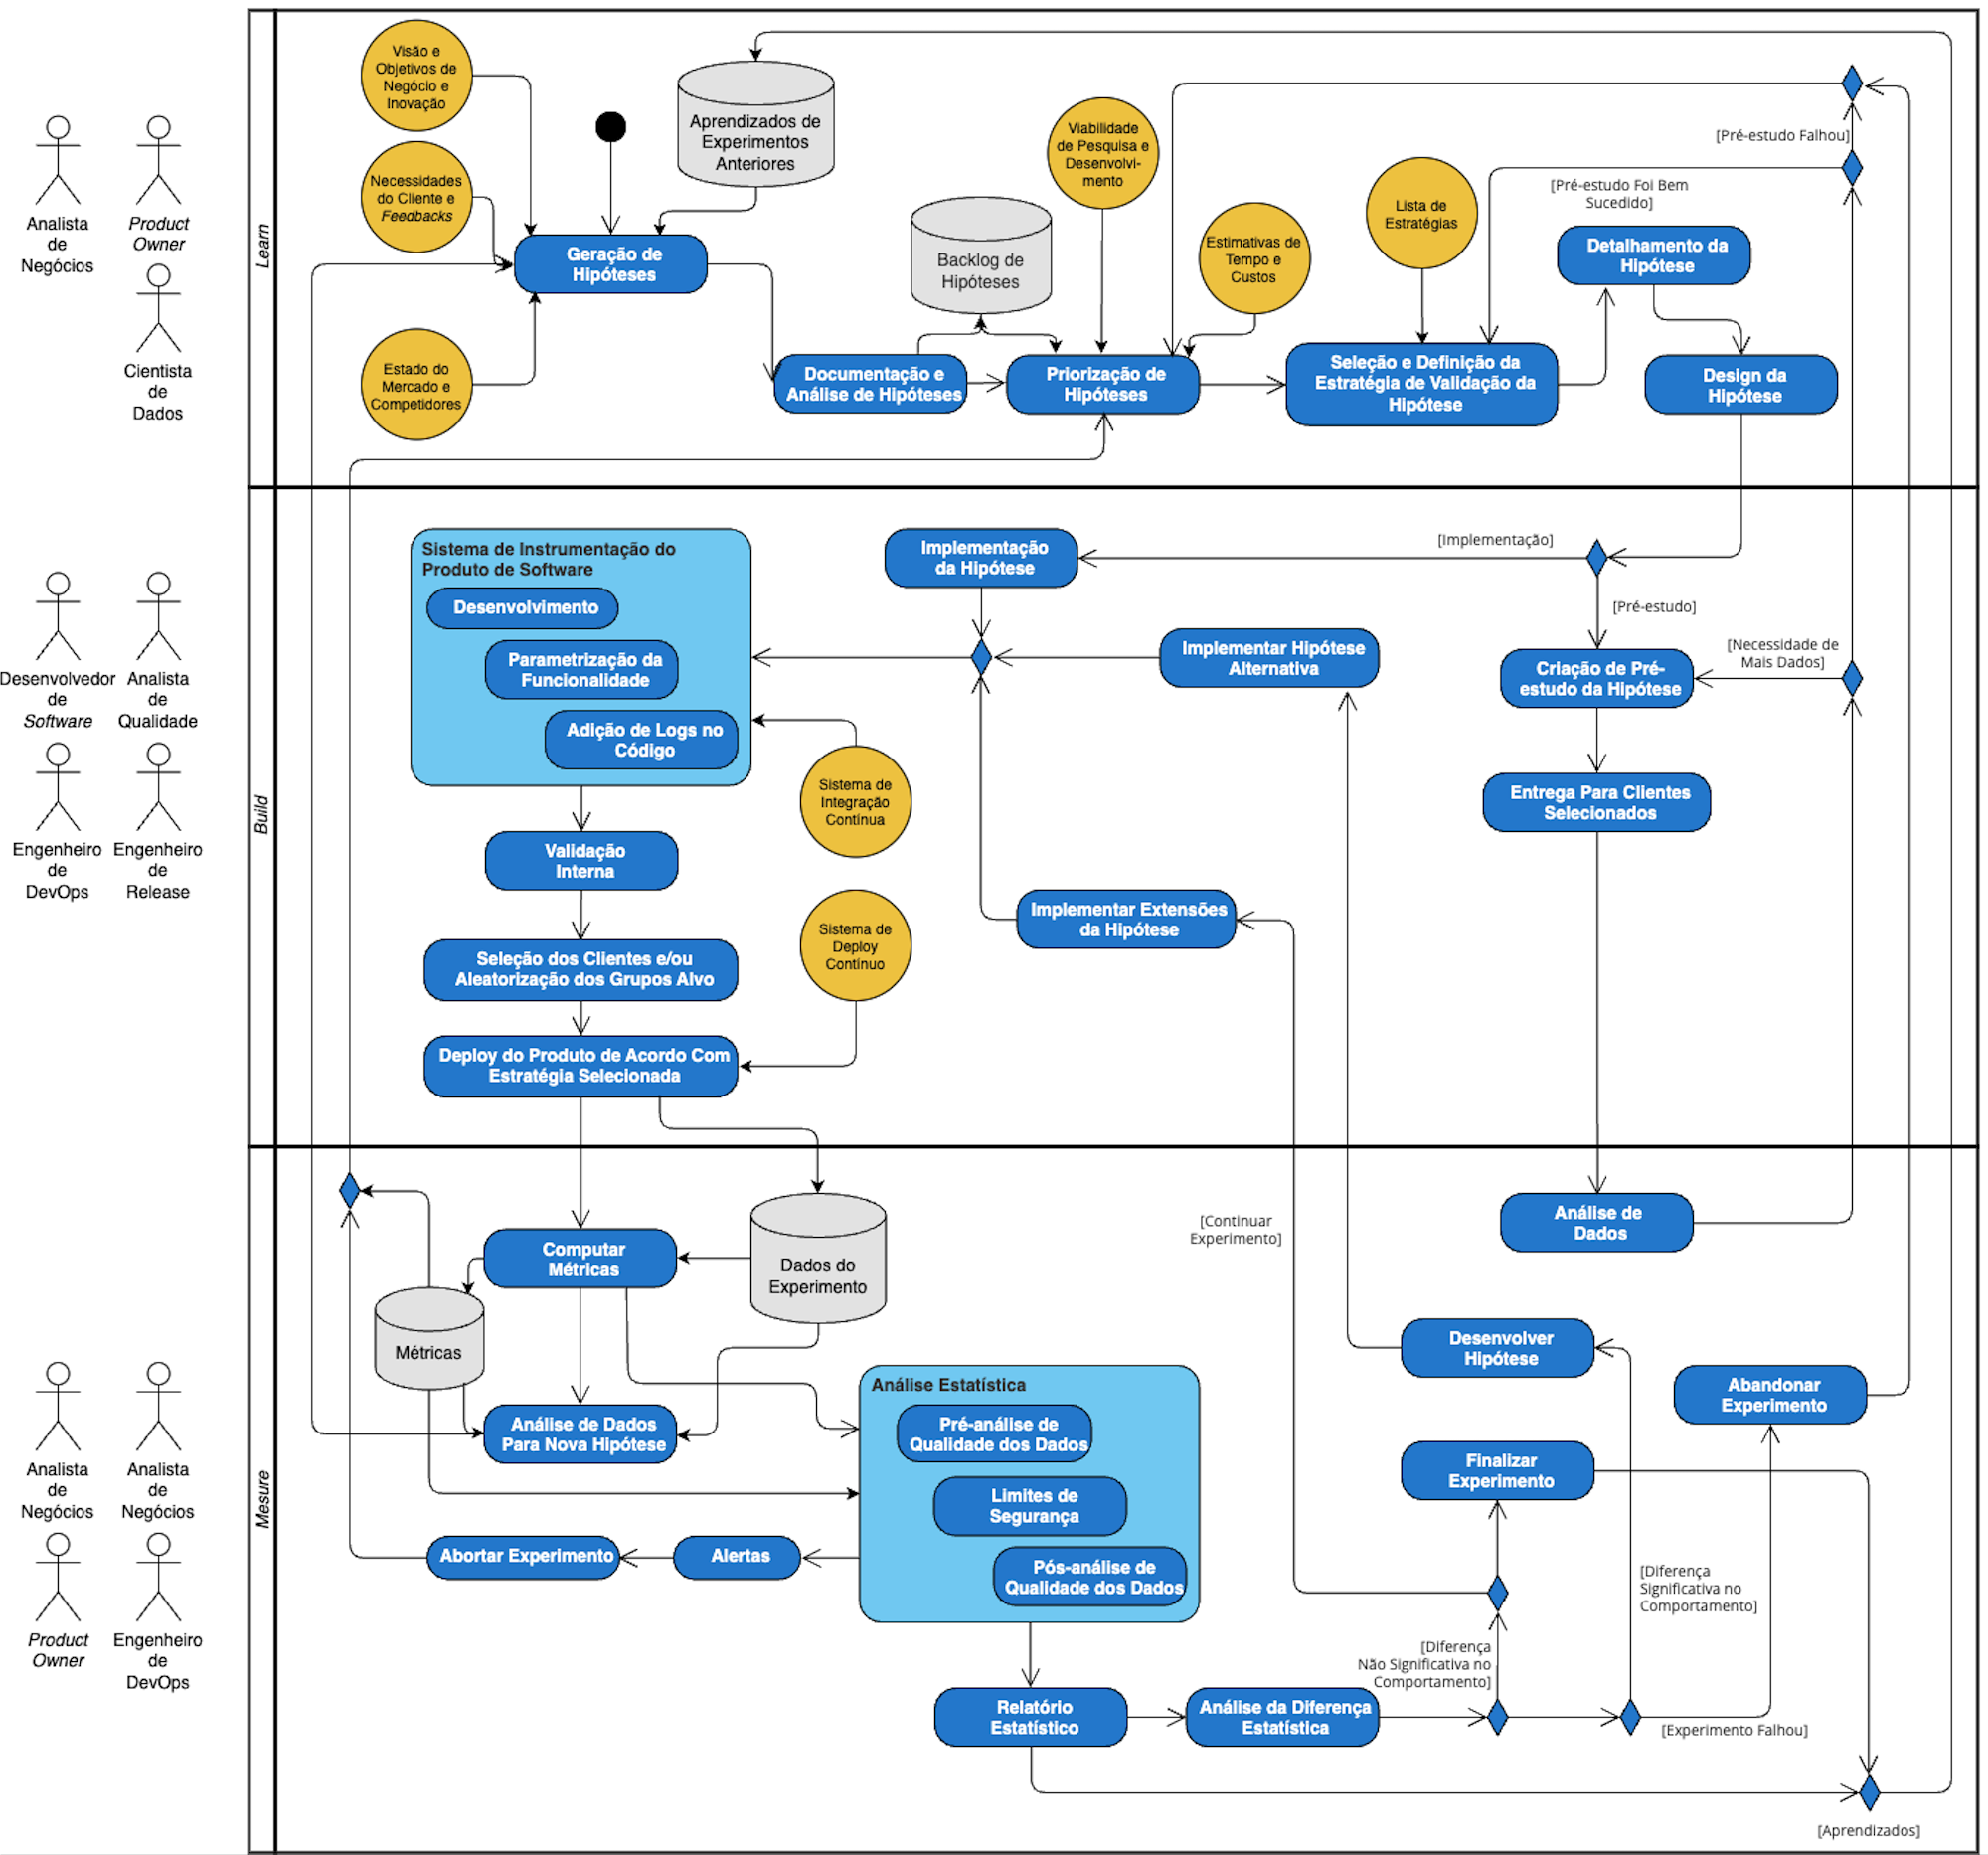
\includegraphics[width=1\linewidth]{figuras/combined_ce_process.png}
\text{Fonte: Adaptado de \citeonline{erthal_characterization_2023}}
\label{fig:erthal-process}
\end{figure}

% O artigo \citeonline{erthal_characterization_2023} realiza um trabalho minucioso na caracterização da literatura, trazendo diversos estudos primários e modelos já existentes. Por isso, o processo proposto pelos autores se apresenta como uma fonte confiável de referência. Desta forma, optou-se por guiar as atividades a serem realizadas no Estudo de Caso desta monografia a partir do modelo apresentado, analisando o processo de desenvolvimento atual do produto analisado e identificando atividades faltantes ou melhorias para as já existentes.

\section{Análise Estatística de Dados}
\label{sec:ref-analise-dados}

Esta seção aborda os conceitos e metodologias do domínio da estatística necessários para testes de hipótese. O propósito é realizar uma contextualização nas metodologias que serão empregadas durante a análise dos dados quantitativos durante o estudo de caso deste trabalho.

Para a realização de decisões estatísticas, são formuladas \textbf{hipóteses estatísticas}, que servem para guiar a avaliação de amostras de dados coletadas, bem como tomadas de decisão. Em um experimento, estas hipóteses são definidas na fase de planejamento e devem guiar todo o processo de experimentação. Quando desejamos analisar a diferença entre duas amostras, formulamos hipóteses para que as mesmas sejam aceitas ou rejeitadas, iniciando pela proposição de que não há diferença entre as amostras. Esta hipótese inicial é chamada de \textbf{hipótese nula}, já as demais são chamadas \textbf{hipóteses alternativas} \cite{juristo_basics_2001}.

Visando rejeitar a hipótese nula, se analisa a diferença entre as amostras coletadas e, caso esta seja considerável, entende-se que é \textit{significativa} e suficiente para a tomada de decisão. As maneiras pelas quais medimos este nível de diferença são chamadas de \textbf{testes de significância} ou \textbf{regras de decisão} \cite{juristo_basics_2001}.

Quando a hipótese nula é rejeitada quando não deveria, se caracteriza um \textbf{erro do tipo I}, ou seja, um falso positivo. Quando o contrário acontece e a hipótese nula é aceita quando não deveria, um falso negativo, se tem um \textbf{erro do tipo II}. O risco de acontecimento de ambos os erros podem ser mitigados através do aumento da amostra, porém, isso nem sempre é possivel \cite{wohlin_experimentation_2012}.

Ao se realizar um teste de hipótese, é definido um \textbf{nível de significância}, que seria o nível máximo que o pesquisador está disposto a arriscar cometer um erro de tipo I. Ou seja, caso seja definido um nível de 0.05 (5\%), é aceito que a cada 100 análises, 5 rejeitarão a hipótese nula quando ela deveria ser aceita. Normalmente este nível é representado pela letra grega alfa (\( \alpha \)) \cite{juristo_basics_2001}.

Já os erros de tipo II dependem de outros fatores, como a diferença nas observações das diferentes hipóteses e poder do teste estatístico, representada por beta (\( \beta \)). O \textbf{poder de um teste} é definido pela probabilidade de se rejeitar corretamente a hipótese nula, representado por 1 - \( \beta \). Por exemplo, um nível de poder de 0.4 indica que se um experimento for executado 10 vezes um efeito causado por algum fator alternativo será descoberto apenas em 4 delas \cite{juristo_basics_2001}.

\subsection{Estatística Descritiva}
\label{subsec:descritiva}

Após a coleta dos dados, pode se utilizar de métodos de estatística descritiva para se apresentar e descrever estes conjuntos, visando entender sua natureza e identificar anomalias. O objetivo é observar a distribuição do conjunto, se há dados que podem ser desconsiderados e decidir o teste de hipótese mais adequado para a comparação das amostras \cite{wohlin_experimentation_2012}.

\subsubsection{Medidas de Tendência Central e de Distribuição}

\citeonline{wohlin_experimentation_2012} definem que as medidas de tendência central visam apontar o centro do conjunto de dados, e que para isso utilizam os valores de \textbf{média (\( \overline{x} \))}, que é soma dos valores divida pela sua quantidade, \textbf{moda}, que se trata do valor mais recorrente do conjunto e \textbf{mediana (\( \tilde{x} \))}, que seria o valor encontrado no meio do conjunto após sua ordenação.

A mediana, também pode ser representada como \(x_{50\%}\), o que indica que ela é o percentil 50\%. Um \textbf{percentil} \(x_p\) indica o valor abaixo do qual \(p\%\) dos dados se encontram. Existem casos especiais de percentis chamados \textbf{quartis}, que dividem os dados em quatro partes iguais: o primeiro quartil (Q1 ou \(l_q\)) marca o valor abaixo do qual se encontra 25\% dos dados amostrais, e o terceiro quartil (Q3 ou \(u_q\)), 75\% \cite{wohlin_experimentation_2012}.

\citeonline{wohlin_experimentation_2012} também apresentam as medidas de distribuição, que por sua vez visam apresentar quão concentrado está o conjunto de dados. Para isto utiliza-se de medidas como a \textbf{variância (\textit{\( s^2 \)})}, o \textbf{desvio padrão (\textit{s})} e a \textbf{amplitude}. A amplitude é a distância entre os valores máximos e mínimos do conjunto. A variância é a média dos quadrados das distâncias entre os valores da amostra e sua média. O desvio padrão é a raiz quadrada da variância. Então, sendo \textit{s} o desvio padrão, \( s^2 \) a variância, \textit{n} o número de dados observados e \(x_i \) o i-ésimo dado observado, as medidas citadas podem ser representadas da seguinte forma:
\[
\text{amplitude} = x_{\text{max}} - x_{\text{min}}
\]

\[
\textit{s} = \sqrt{s^2}
\]

\[
s^2 = \frac{1}{n} \sum_{i=1}^{n} (x_i - \bar{x})^2
\]


\subsubsection{Representação Gráfica}

Além das medidas existentes na estatística descritiva, \citeonline{wohlin_experimentation_2012} também abordam como a representação gráfica do conjunto de dados pode ajudar a entender a natureza do conjunto, ajudando a identificar visualmente \textit{outliers}, que são pontos que diferem muito do conjunto e atrapalhar a análise. Os autores apresentam diferentes tipos de gráficos que podem ser úteis para esta prática, alguns deles são:

\begin{itemize}
    \item \textbf{Gráfico de Dispersão:} apresenta amostras pareadas em duas dimensões, permitindo identificar dependências, padrões lineares e \textit{outliers} (exemplificado na Figura \ref{fig:scatterplot});
    \item \textbf{Gráfico de Caixa (\textit{Box Plot}):} permite se visualizar a dispersão e a assimetria dos dados. Apresenta a mediana, o primeiro e o terceiro quartis (exemplificado na Figura \ref{fig:boxplot}). A largura da caixa é \textit{d} onde \textit{d} = \(u_q\) - \(l_q\). O gráfico é delimitado por suas caudas (ou bigodes), que se estendem até 1,5 vezes o comprimento da caixa a partir dos quartis. Esta delimitação serve para representar a área onde, teoricamente, todos os dados conjunto deveriam ser encontrados, ou seja, aqueles fora desta região são considerados \textit{outliers}; e
    \item \textbf{Histograma:} representa a distribuição dos dados e mostra a frequência de intervalos de valores (exemplificado na Figura \ref{fig:histogram}). Cada barra representa a quantidade de dados dentro de um intervalo específico e sua altura indica a frequência de dados dentro deste intervalo. Isto permite observar facilmente a distribuição que os dados seguem ou se existem picos ou lacunas significativas.
\end{itemize}

\begin{figure}
    \centering
    
    \caption{Exemplo de Gráfico de Dispersão}
    
    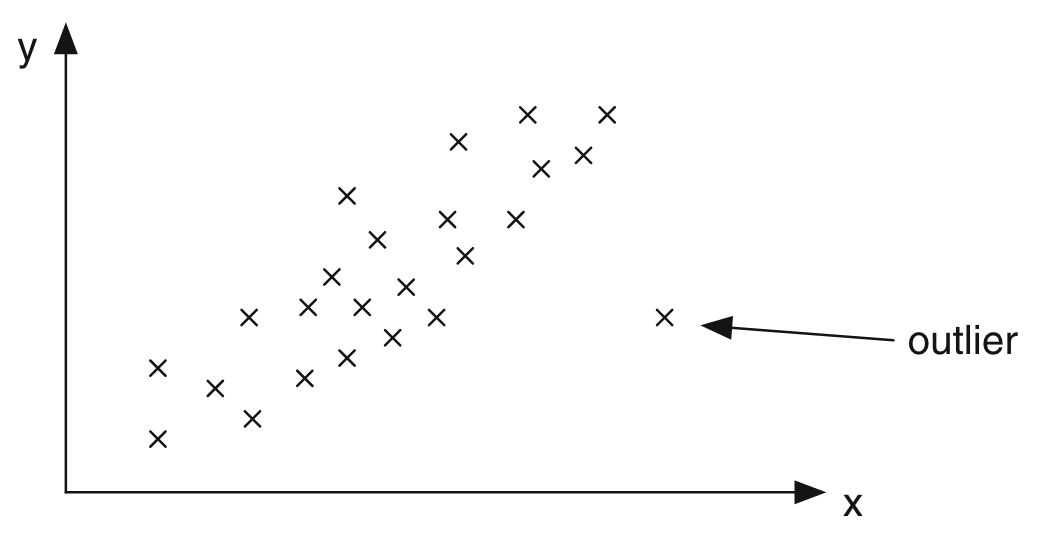
\includegraphics[width=0.7\linewidth]{figuras/scatter.png}
    
    \text{Fonte: \citeonline{wohlin_experimentation_2012}}
    
    \label{fig:scatterplot}
\end{figure}

\begin{figure}
    \centering
    
    \caption{Exemplo de Gráfico de Caixa}
    
    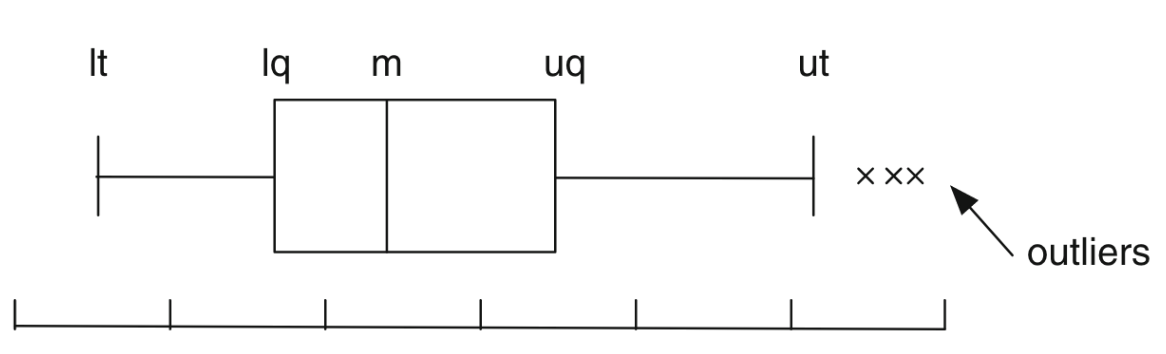
\includegraphics[width=0.7\linewidth]{figuras/boxplot.png}
    
    \text{Fonte: \citeonline{wohlin_experimentation_2012}}
    
    \label{fig:boxplot}
\end{figure}

\begin{figure}
    \centering
    
    \caption{Exemplo de Histograma}
    
    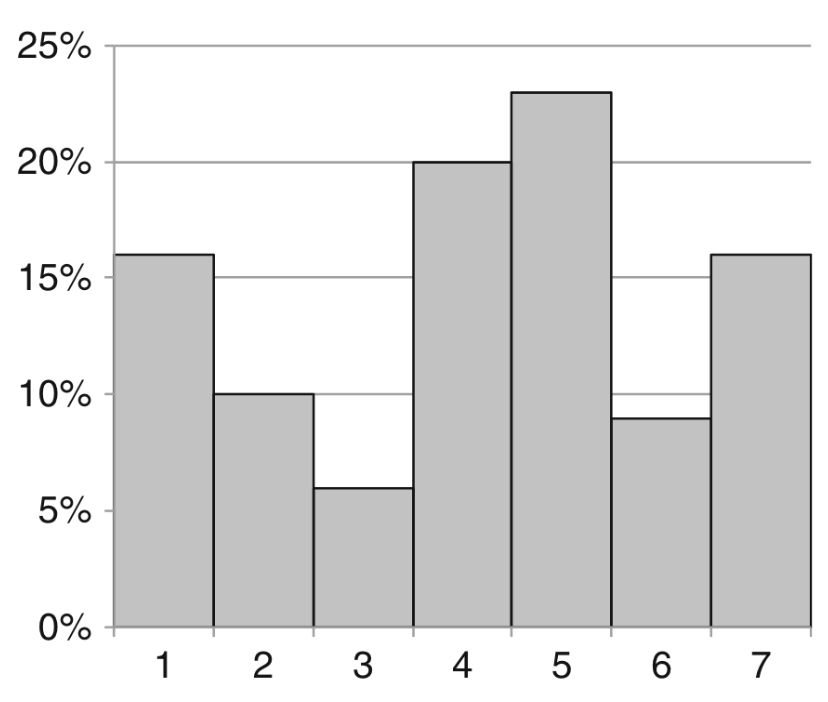
\includegraphics[width=0.5\linewidth]{figuras/histogram.png}
    
    \text{Fonte: \citeonline{wohlin_experimentation_2012}}
    
    \label{fig:histogram}
\end{figure}

A identificação dos \textit{outliers} por meio destes processos de representação gráfica é crucial para a chamada \textbf{redução dos dados}. Valores que se desviam significativamente dos demais podem comprometer a qualidade do conjunto de dados e prejudicar a análise. Portanto, é fundamental identificá-los e avaliar a necessidade de sua remoção. Caso um valor resulte de um evento raro, ele pode ser removido; no entanto, um ponto que revele informações valiosas deve ser analisado separadamente \cite{wohlin_experimentation_2012}.

\subsection{Teste de Hipóteses}

O objetivo de um teste de hipótese é verificar se é possível rejeitar uma hipótese nula a partir da análise de um determinado conjunto de dados. Ou seja, \(x_i \) descreve determinadas propriedades e o teste visa negar estas características com determinado nível de significância \cite{wohlin_experimentation_2012}. 

Um teste de hipótese pode ser paramétrico ou não paramétrico. Os paramétricos se baseiam em modelos que pressupõem a distribuição dos dados coletados, já os não paramétricos não fazem suposições \cite{juristo_basics_2001}. Um destes pressupostos pode ser que o conjunto está normalmente distribuído. Esta distribuição é caracterizada por uma curva simétrica em formato de sino e isso pode ser verificado através de diferentes tipos de gráficos \cite{wohlin_experimentation_2012}.

A seguir serão apresentados alguns testes de hipótese existentes, métodos que se adequam ao contexto deste trabalho, onde serão avaliadas amostras independentes de dados, que podem ser grandes ou pequenas e que podem ter sua distribuição normal ou não.

\subsubsection{Teste Z}

Este é um teste paramétrico para quando trabalhamos com amostras grandes (\(n \geq 30\)). Nestes conjuntos a distribuição das médias amostrais tende a ser normal, o que significa que a média das amostras se aproxima da média da população total, assim como o desvio padrão. Isso facilita a inferência sobre a população total com base nos dados coletados \cite{juristo_basics_2001}.

Utiliza-se da regra de decisão de diferença entre médias para se avaliar a significância da diferença entre as duas amostras coletadas. Caso essa diferença não seja significativa, se entende que a diferença observada pode ser atribuída ao acaso, o que nos leva a não rejeitar a hipótese nula. O valor responsável por nos dizer o valor dessa significância é chamada de z (ou \textit{z-score}) \cite{juristo_basics_2001}.

\citeonline{juristo_basics_2001} demonstram que para calcular o valor de \textit{z}, primeiro realizamos um processo de normalização dos valores da amostra analisada, para que possamos distribuir nossos dados na distribuição padrão da variável \textit{z}, apresentada na Figura \ref{fig:z-score} (onde a média é 0 e o desvio padrão é 1). Nesta curva, o valor central é 0, e o eixo x tem como medida o desvio padrão, que no caso é 1, o valor de \textit{z} vai nos dizer quantos desvios padrões um dado valor se distancia da média, que é 0. 

Para calcular o valor de \textit{z} se utiliza a seguinte fórmula, onde \textit{S} é alguma medida da amostra (média, desvio padrão, etc), e \(\mu_S\) e \(\sigma_S\) são respectivamente a média e o desvio padrão desta medida:

\[
z = \frac{S - \mu_S}{\sigma_S}
\]

Assim, os valores mais distantes se encontram nas regiões críticas, como apresentado na Figure \ref{fig:z-score}, que demonstra que os valores encontrados nelas teriam um \textit{z-score} maior que 1.96 ou menor que -1.96 (no exemplo o nível de significância é de 0.05, ou 5\%).



\begin{figure}
    \centering
    
    \caption{Distribuição da Estatística Z}
    
    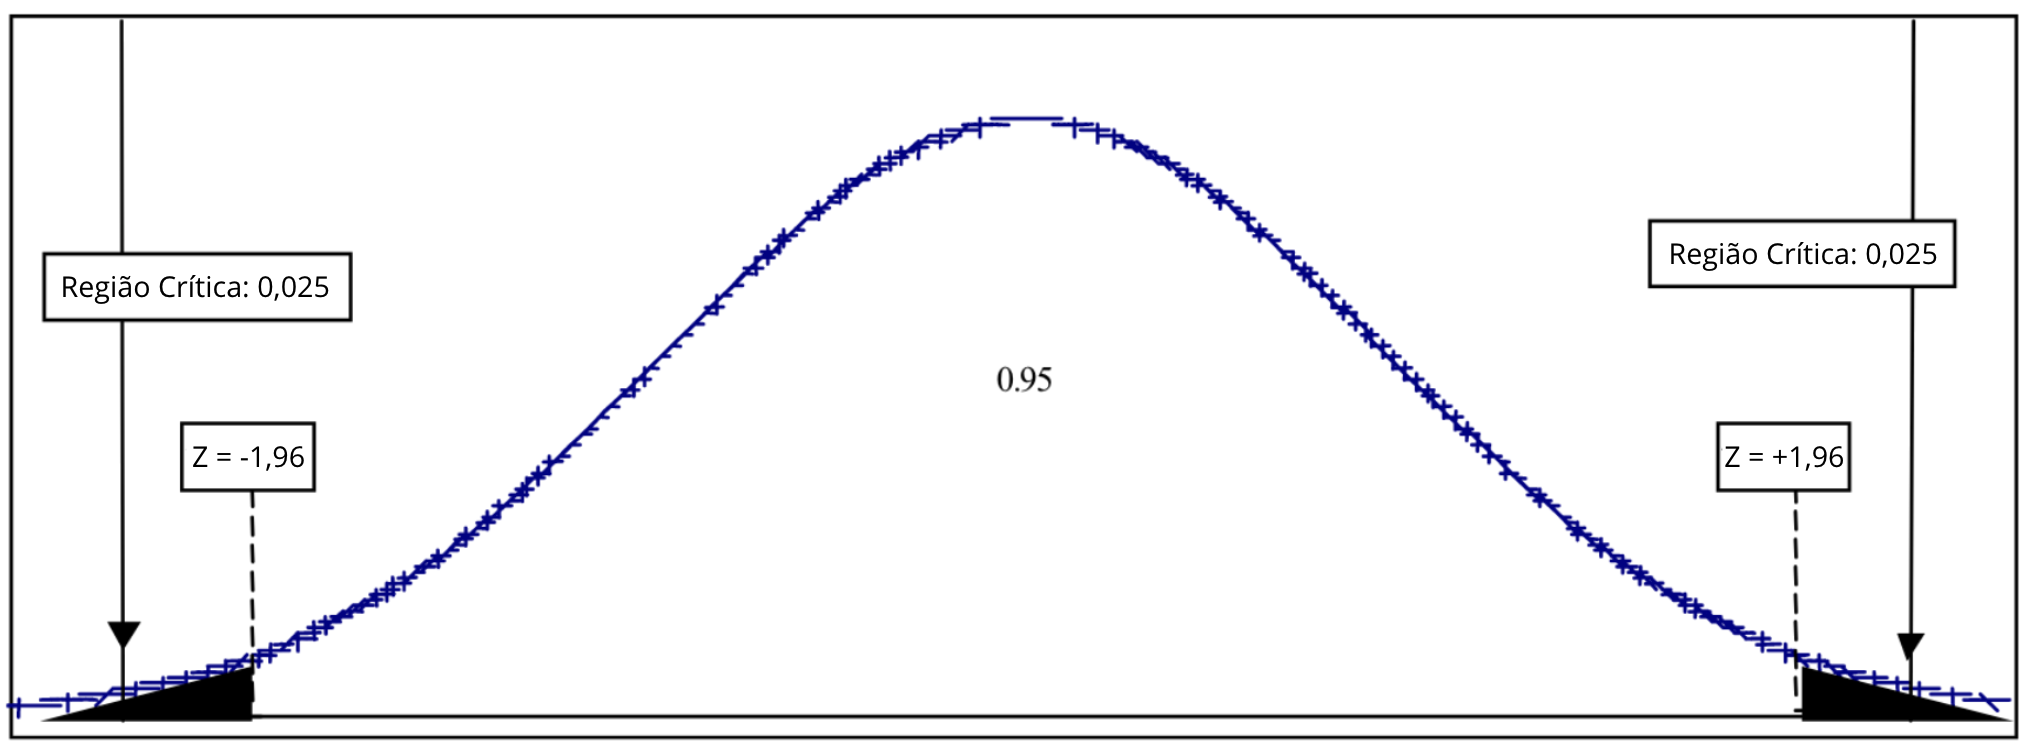
\includegraphics[width=1\linewidth]{figuras/z_distr.png}
    
    \text{Fonte: Adaptado de \citeonline{juristo_basics_2001}}
    
    \label{fig:z-score}
\end{figure}

\subsubsection{Teste T de Student}
\label{subsec:t-test}

Este também é um teste paramétrico, onde se espera que a amostra coletada se aproxime da distribuição normal. É uma alternativa para quando se lida com conjuntos pequenos de dados. A distribuição do valor de \textit{t} é bem parecida com a distribuição normal, porém depende do grau de liberdade da amostra, que é representado por \textit{v}. Quanto maior o grau de liberdade, mais a curva da distribuição se aproxima da curva normal \cite{juristo_basics_2001}. Esse teste é comumente utilizado para comparar duas amostras independentes de variáveis numéricas \cite{wohlin_experimentation_2012}.

A curtose é uma característica da estatística descritiva que define o achatamento da curva de uma distribuição. A curtose de uma distribuição normal é 0, indicando uma distribuição com um formato de sino padrão. Em contraste, a curtose de uma distribuição t de Student tende a ser cada vez mais negativa conforme o grau de liberdade diminui \cite{juristo_basics_2001}. Isso significa que, com menos graus de liberdade, a distribuição t apresenta caudas mais largas e uma forma mais achatada, refletindo a maior variabilidade e incerteza associadas a amostras menores, vide a Figura\ref{fig:t-statistic}.

O grau de liberdade é calculado a partir da quantidade de amostras a serem testadas e seus respectivos tamanhos, sendo uma amostra \textit{v} = \textit{n} - 1, para duas amostras \textit{v} = \textit{\(n_1\)} + \textit{\(n_2\)} - 2 e assim sucessivamente \cite{juristo_basics_2001}.



\begin{figure}
    \centering
    
    \caption{Distribuição de T Para Diferentes Graus de Liberdade}
    
    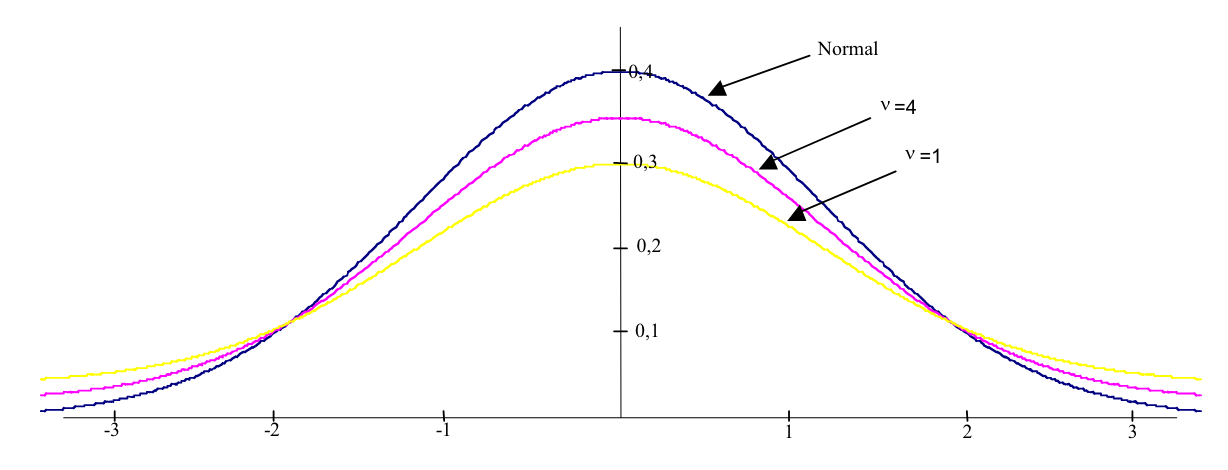
\includegraphics[width=1\linewidth]{figuras/t-statistic.png}
    
    \text{Fonte: \citeonline{juristo_basics_2001}}
    
    \label{fig:t-statistic}
\end{figure}


Para se calcular o valor \textit{t} utiliza-se a fórmula:

\[
t = \frac{\bar{x} - \mu}{s / \sqrt{n}}
\]

onde \(\bar{x}\) é a média amostral, \(\mu\) é a média da população (ou a média de outra amostra), \(s\) é o desvio padrão amostral e \(n\) é o tamanho da amostra. O valor calculado de t é então comparado com os valores críticos da tabela t, que são ajustados para diferentes níveis de significância e graus de liberdade. Esses valores críticos ajudam a determinar se a diferença observada é estatisticamente significativa. A tabela t de Student é gerada a partir de cálculos que levam em consideração a distribuição das amostras \cite{juristo_basics_2001}.




\subsubsection{Teste de Mann-Whitney U}
\label{subsec:u-test}

O teste de Mann-Whitney U, também conhecido como teste U, é uma alternativa não paramétrica para a análise de duas amostras. Este teste não assume que os dados seguem uma distribuição normal, tornando-o mais flexível e aplicável a dados medidos em escalas ordinais. O teste é utilizado para determinar se há uma diferença significativa entre duas amostras independentes \cite{wohlin_experimentation_2012}.

\citeonline{juristo_basics_2001} demonstram que para se realizar o teste de Mann-Whitney U, as observações das duas amostras são organizadas em ordem crescente e substituídas pelos seus postos ou \textit{ranks}. Quando há empates, cada valor é substituído pela média dos \textit{ranks} correspondentes. A soma dos \textit{ranks} para cada amostra é calculada e utilizada para determinar o valor da estatística \textit{u}. A fórmula para o cálculo de \textit{u} é:

\[
u = r_1 - \frac{n_1 (n_1 + 1)}{2}
\]

onde \(r_1\) é a soma dos \textit{ranks} da primeira amostra e \(n_1\) é o número de observações na primeira amostra. A distribuição amostral de \(u\) é simétrica e, quando o tamanho das amostras é suficientemente grande (geralmente \(n_1 \geq 8\) e \(n_2 \geq 8\)), a distribuição de \(u\) pode ser aproximada por uma distribuição normal com média (\(\bar{x}\)) e variância (\textit{s}) dadas por:

\[
\bar{x} = \frac{N_1 N_2}{2}
\]
\[
\text{s} = \frac{n_1 n_2 (n_1 + n_2 + 1)}{12}
\]

O valor \(z\) é calculado como:

\[
z = \frac{u - \bar{x}}{s}
\]

Esse valor \(z\) é então comparado com os valores críticos da tabela padrão normal para determinar se a diferença observada entre as amostras é estatisticamente significativa. Se \(z\) cair fora do intervalo crítico definido (por exemplo, -1.96 a 1.96 para um nível de significância de 0.05), rejeita-se a hipótese nula e conclui-se que há uma diferença significativa entre as amostras \cite{juristo_basics_2001}.

\subsubsection{Teste Qui-Quadrado}
\label{subsec:chi-square}

O teste qui-quadrado também é um teste não paramétrico. É utilizado para analisar a diferença entre as frequências observadas e esperadas de uma variável categórica. O objetivo do teste é verificar se há uma diferença significativa entre as frequências esperadas, sob uma hipótese nula \(h_0\), e as frequências observadas. É um teste indicado para amostras grandes, diferindo do Mann-Whitney, que é mais apropriado para amostras pequenas \cite{juristo_basics_2001}. Para realização deste teste se utiliza a estatística qui-quadrado (\(\chi^2\)), que é calculada usando a seguinte fórmula:

\[
\chi^2 = \sum_{i=1}^{k} \frac{(o_i - e_i)^2}{e_i}
\]

onde \(o_i\) são as frequências observadas, \(e_i\) são as frequências esperadas sob a hipótese nula, e \(k\) é o número de eventos ou categorias. O valor calculado de \(\chi^2\) é então comparado a um valor crítico da tabela qui-quadrado, que varia de acordo com o número de graus de liberdade (\(\nu = k - 1\)) e o nível de significância escolhido \cite{juristo_basics_2001}.

Se o valor calculado de \(\chi^2\) for maior que o valor crítico da tabela (como \(\chi^2_{0.95}\), para um nível de significância de 0,05), a hipótese nula é rejeitada, indicando uma diferença significativa entre as frequências observadas e esperadas. Caso contrário, não há evidência suficiente para rejeitar a hipótese nula \cite{juristo_basics_2001}.


\section{Resumo do Capítulo}

Este capítulo abordou os principais conceitos utilizados no desenvolvimento deste estudo, incluindo as metodologias de pesquisa, os modelos nos quais a proposta do estudo se baseou, bem como as arquiteturas e técnicas escolhidas para sua implementação. Dentre estas se destacam as \textit{feature toggles} e os conceitos e métodos estatísticos que fundamentarão os testes de hipótese à serem realizados.

Além disso, foram conceituadas e apresentadas as estratégias de investigação a utilizadas neste trabalho, como a Revisão Sistemática da Literatura, que orientou o estudo realizado para desenvolvimento deste trabalho, o Estudo de Caso, cujos processos serão executados na segunda fase desta monografia, e, por fim, o Experimento, que é o principal objeto do processo proposto de experimentação contínua.

Com base em normas técnicas, também foram caracterizadas a qualidade do \textit{software} e a qualidade em uso. Essas normas apresentam critérios e diretrizes para avaliar a qualidade de um produto de \textit{software}, os quais estão diretamente relacionados aos experimentos, que têm como objetivo aumentar e assegurar a qualidade de um sistema.

\chapter{Revisão Estruturada da Literatura}   
\label{ch:revisao}

Neste capítulo, são detalhados os passos realizados para selecionar o material bibliográfico deste trabalho. Para realização desta busca, foi utilizada a base de dados Scopus, já que a mesma indexa uma grande variedade das principais revistas e conferências relevantes na academia \cite{elsevier2022}.

\section{Planejamento e Protocolo}
\label{sec:rsl-protocolo}

Inicialmente, realizou-se uma busca \textit{ad hoc} por estudos que tratassem da experimentação contínua com o objetivo de encontrar materiais que caracterizassem a literatura do tema em questão. O conjunto encontrado é apresentado na Tabela \ref{tab:conjunto-inicial}.

\begin{table}[]
\centering
\caption{Conjunto Inicial de Artigos}
    \begin{tabular}{|p{.5cm}|p{6cm}|p{6cm}|p{1.75cm}|}
        \hline
        Nº & Título & Fonte de Publicação & Referência \\ \hline
        1 & \textit{Characterizing Experimentation in Continuous Deployment: A Case Study on Bing} & \textit{2017 IEEE/ACM 39th International Conference on Software Engineering: Software Engineering in Practice Track (ICSE-SEIP)} & \cite{kevic_characterizing_2017} \\ \hline
        2 & \textit{Controlled Experiments on the Web: Survey and Practical Guide} & \textit{KDD '07: Proceedings of the 13th ACM SIGKDD international conference on Knowledge discovery and data mining} & \cite{kohavi_controlled_2009} \\  \hline
        3 & \textit{The Evolution of Continuous Experimentation in Software Product Development: From Data to a Data-Driven Organization at Scale} & \textit{2017 IEEE/ACM 39th International Conference on Software Engineering (ICSE)} & \cite{fabijan_evolution_2017} \\ \hline
        4 & \textit{Designing and Deploying Online Field Experiments} & \textit{WWW '14: Proceedings of the 23rd international conference on World wide web} & \cite{bakshy_designing_2014} \\ \hline
        5 & \textit{Building Products as Innovation Experiment Systems} & \textit{International Conference on Software Business (ICSOB 2012)} & \cite{van_der_aalst_building_2012} \\ \hline
        6 & \textit{Overlapping Experiment Infrastructure: More, Better, Faster Experimentation} & \textit{KDD '10: Proceedings of the 16th ACM SIGKDD international conference on Knowledge discovery and data mining} & \cite{tang_overlapping_2010} \\ \hline
        7 & \textit{Characterization of Continuous Experimentation in Software Engineering: Expressions, models, and strategies} & \textit{Science of Computer Programming} & \cite{erthal_characterization_2023} \\ \hline
    \end{tabular}

    \begin{center}
        \text{Fonte: Author}
        
    \end{center}

\label{tab:conjunto-inicial}
\end{table}   

Após a realização destas leituras, optou-se por escolher um dos artigos como estudo de controle para uma posterior busca estruturada na literatura, isto é, ao executar a \textit{string} de busca, o mesmo deveria ser retornado, ajudando a entender como as variações dos termos da \textit{string} afetam os resultados encontrados. Esta escolha não foi casual, porém estratégica, por se tratar de um estudo secundário, publicado em revista, e que tem como objetivo caracterizar o corpo de conhecimento existente na área da experimentação, trazendo diferentes modelos, expressões e estratégias encontradas nos estudos primários analisados, publicados entre os anos de 2015 e 2022 \cite{erthal_characterization_2023}.

% Publicado recentemente, no ano anterior ao desenvolvimento desta monografia, aborda diversas questões que podem servir de investigação para um trabalho de graduação na área do desenvolvimento orientado a dados. Para seguir com a revisão da literatura de forma estruturada, optou-se por adaptar a busca realizado no artigo, olhando para publicações realizadas a partir do ano de 2023 e reformulando o método de pesquisa utilizado pelos autores.

Escolhido o estudo de controle, partiu-se para a formalização do protocolo de pesquisa. Apesar deste trabalho não se tratar de uma revisão sistemática, utilizou-se da estrutura proposta por \citeonline{kitchenham_rsl}, o que torna possível a replicabilidade e a aferência dos resultados. O intuito principal da pesquisa foi encontrar outros trabalhos que caracterizassem a literatura na área da experimentação, por isso o foco em estudos secundários/terciários, levantando, desta forma, um conjunto que pudesse servir de semente para um processo de \textit{snowballing}. O protocolo consolidado é apresentado na Tabela \ref{tab:protocolo-busca}.

Definiu-se que o \textit{snowballing} seria realizado selecionando referências citadas nestes primeiros artigos filtrados pelos critérios do protocolo de revisão da literatura, especificamente aquelas que indicassem abordar algum tópico pertinente às questões de pesquisa deste trabalho.


\begin{table}[]
\centering
\caption{Protocolo de Busca}
\begin{tabular}{|p{4cm}|p{11cm}|}
\hline
Questões de Pesquisa & 1. Quais são os processos/modelos utilizados no desenvolvimento orientado a dados? \newline 2. Quais são as estratégias utilizadas no desenvolvimento orientado a dados? \newline 3. Quais ferramentas/tecnologias comumente utilizadas na indústria para instrumentalização de experimentos? \newline 4. Quais os principais desafios e problemas reportados? \\ \hline
String de Busca & Ver Tabela \ref{tab:string-busca} \\ \hline
Critérios de Inclusão & 1. O artigo deve conter informações para responder ao menos uma questão de pesquisa. \newline 2. O artigo deve estar no contexto da Experimentação Contínua. \newline 3. O artigo deve ser um estudo secundário ou terciário. \\ \hline
Critérios de Exclusão. & 1. Duplicação/Auto Plágio. \newline 2. O artigo não está em inglês \newline 3. O artigo trata de outro domínio que não o \textit{Web}. \\ \hline
Formulário de Extração de Dados & Q1. Título \newline Q2. Resumo \newline Q3. Ano de Publicação \newline Q4. Fonte de Publicação \newline Q5. Autores \newline Q6. Key-words \newline Q7. Processo/Modelo de Desenvolvimento \newline Q8. Estratégias de Desenvolvimento \newline Q9. Ferramentas/Tecnologias Utilizadas \newline Q10. Principais Desafios Reportados \\ \hline
\end{tabular}
\begin{center}
\text{Fonte: Autor}
    
\end{center}
\label{tab:protocolo-busca}
\end{table}


\section{Estruturação da \textit{String} de Busca}

Para estruturar a delimitação da \textcolor{red}{\st{pesquisa}} \todo[color=yellow]{busca na base digital,} utilizou-se o protocolo PICO, proposto na área da medicina. Procederam-se as adaptações necessárias para o contexto da engenharia de \textit{software}. PICO é um acrônimo para \textit{patient} (população de pacientes), \textit{intervention} (intervenção), \textit{comparison} (comparação) e \textit{outcome} (resultado) e pode ser representado como um gráfico de \textit{Venn}, como observado na figura \ref{fig:pico} \cite{pai_clinical_2004}.




\begin{figure}
    \centering
    \caption{Representação Visual do Protocolo PICO }
    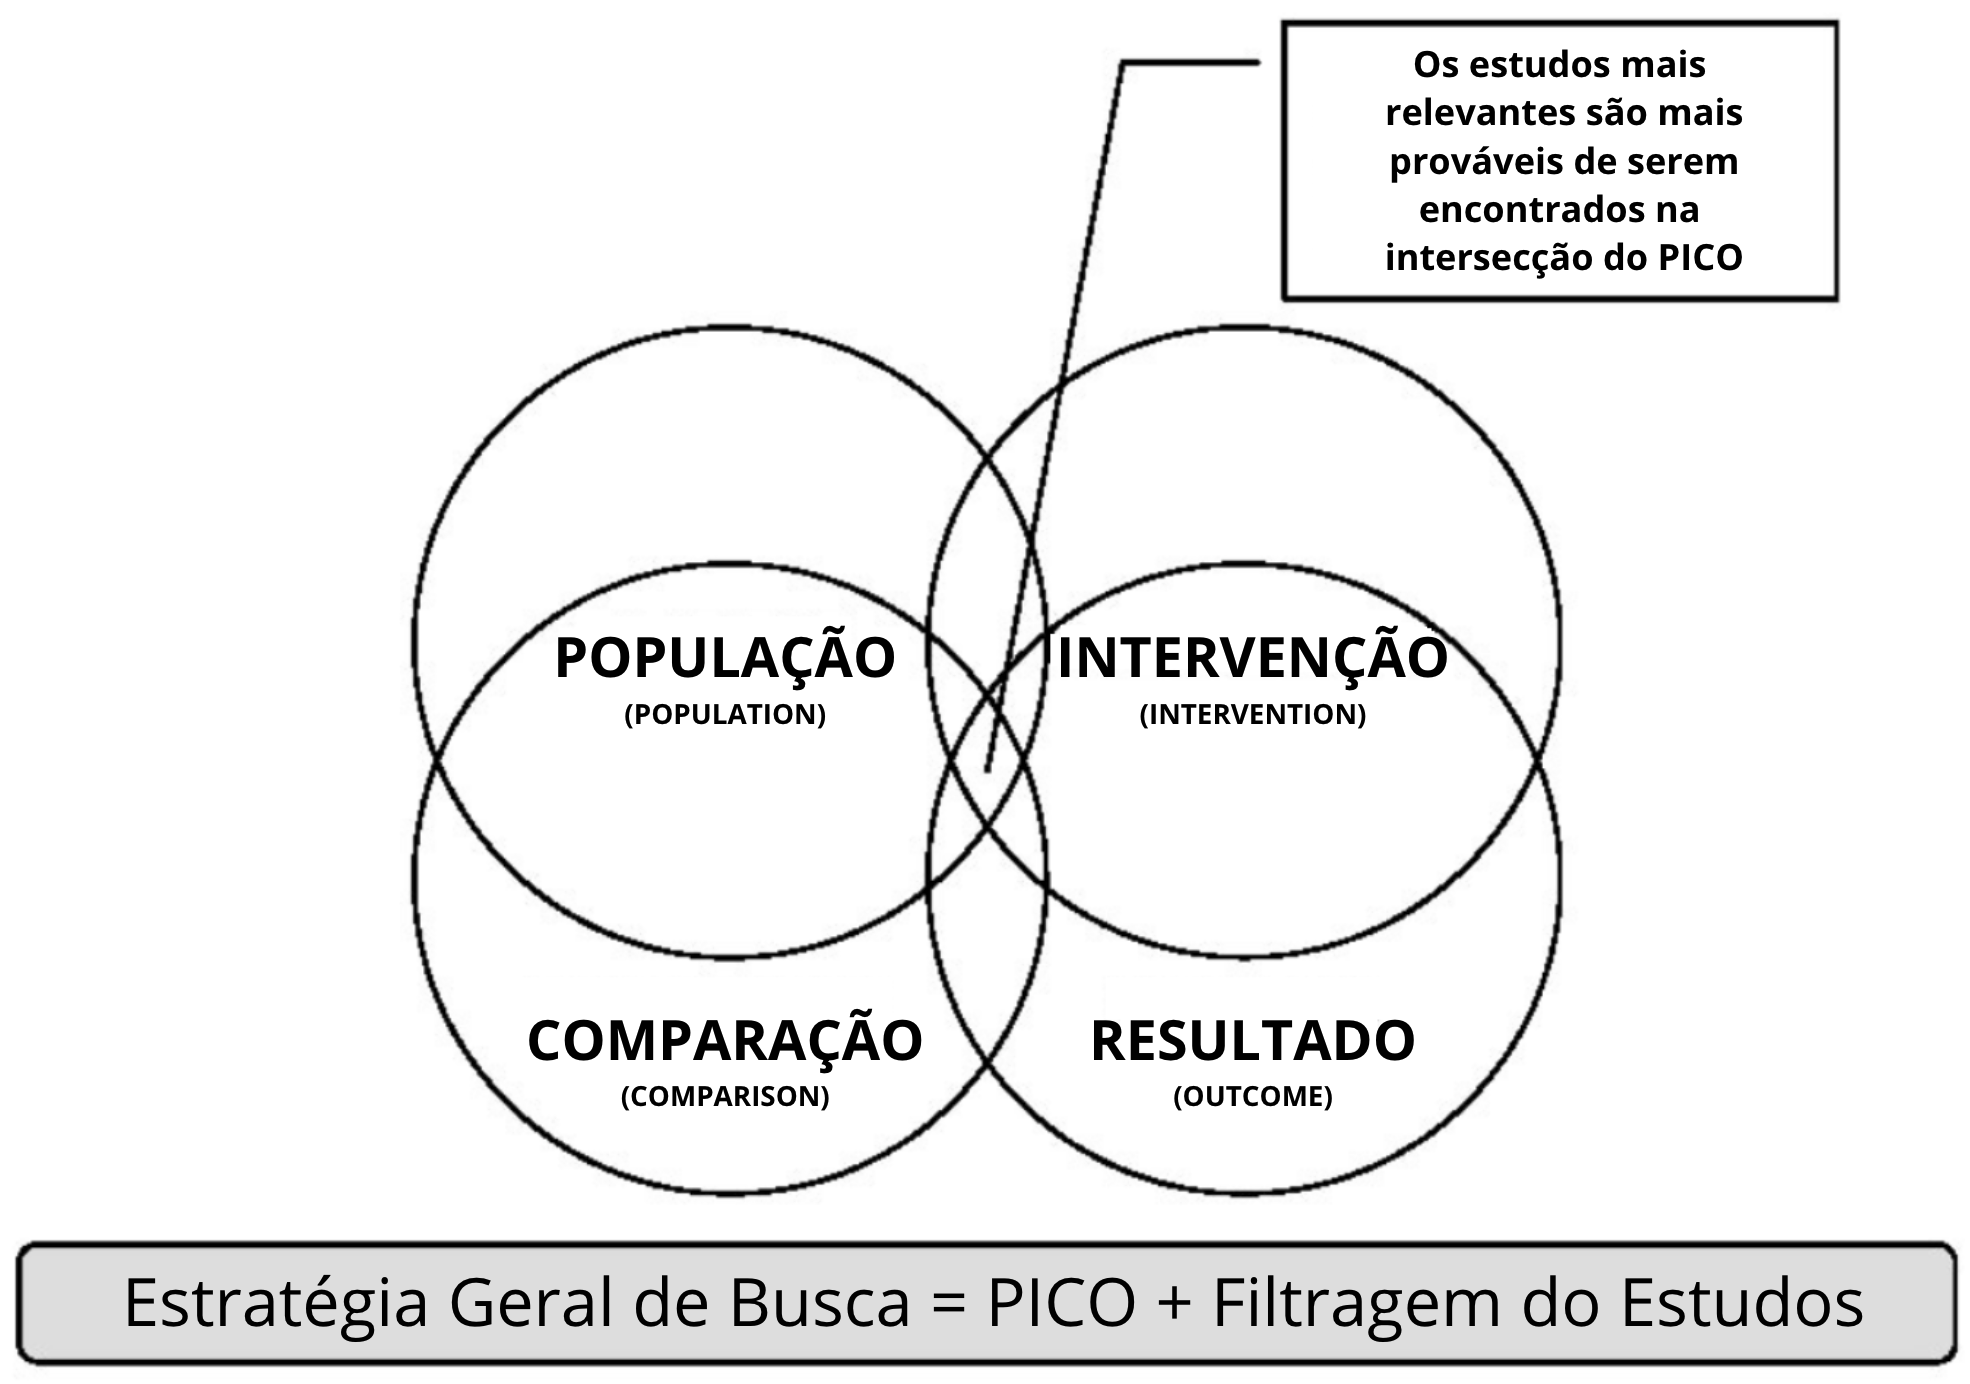
\includegraphics[width=0.75\linewidth]{figuras/PICO.png}
    \text{Fonte: Adaptado de \citeonline{pai_clinical_2004}}
    \label{fig:pico}
\end{figure}

Considerando o contexto do produto investigado nesta monografia, a \textbf{população de pacientes} equivale a sua área específica da engenharia de software, o desenvolvimento \textit{web}. Na medicina, a \textbf{intervenção} se refere ao tratamento a ser aplicado e analisado, então, foram utilizados termos relacionados a experimentação contínua. O \textbf{resultado} representa a saída relatada nos estudos a serem selecionados e, em busca de compreender o estado da arte, foram adicionados termos que representassem estudos secundários e terciários, como revisão da literatura, mapeamento sistemático, etc. Já a \textbf{comparação} seria a adição de outros tipos de intervenção a serem comparadas com a principal. Porém, dado que a área da Engenharia de \textit{Software} ainda é muito nova, o corpo de conhecimento ainda não é tão bem organizado como na medicina, o que impede que esta camada da \textit{string} funcione como proposto na área médica, por isso, não foi utilizada.

Desta forma, os termos utilizados foram gerados a partir da união da \textit{string} de busca do estudo de controle e das expressões que o mesmo trouxe como utilizadas na literatura para se referir à experimentação contínua e tópicos relacionados. A estrutura consolidada é apresentada na Tabela \ref{tab:string-busca}.


\begin{table}[]
\caption{Estrutura dos Termos da String de Busca}
    \begin{tabular}{|p{2cm}|p{3cm}|p{9cm}|}
        \hline
        \textbf{Camada} & \textbf{Palavra Chave} & \textbf{Sinônimos} \\ \hline
        População & \textit{software development} & \textit{software engineering} 
         e \textit{web development} \\ \hline
        Intervenção & \textit{continuous experimentation} & \textit{continuous software experimentation}, \textit{experiment systems}, \textit{data-driven development}, \textit{A/B tests}, \textit{online controlled experiments}, \textit{innovation experiment system}, \textit{experiment-driven software development}, \textit{evidence-based software engineering}, \textit{experimentation system}, \textit{customer-driven development} e \textit{experiment-driven development} \\ \hline
        Resultado & \textit{systematic literature review} & \textit{secondary studies}, \textit{tertiary studies}, \textit{literature review} e \textit{systematic literature mapping} \\ \hline
    \end{tabular}

    \begin{center}
        \text{Fonte: Autor}
        
    \end{center}

\label{tab:string-busca}
\end{table}

Para finalizar, adicionou-se o operador lógico 'AND' para separar cada camada do protocolo e, dentro de cada uma delas, o operador lógico 'OR' para separar as palavras-chave e seus sinônimos. Acrescentou-se também sintaxes específicas da base de dados para realizar o truncamento de termos, a fim de abranger diferentes terminologias para as mesmas palavras chave. Isto resultou na string finalizada da seguinte forma:

\textit{("software development" OR "software engineering" OR "web development") 
AND 
("continuous experimentation" OR "continuous software experimentation" OR "experiment systems" OR "data-driven development" OR "A/B test*" OR "online controlled experiment*" OR "innovation experiment system" OR "experiment-driven software development" OR "evidence-based software engineering" OR "experimentation system" OR "customer-driven development" OR "experiment-driven *") 
AND 
("secondary stud*" OR "tertiary stud*" OR "literature review" OR "systematic literature review" OR "systematic literature mapping" OR "combined process") 
}

\section{Realização da Busca e Seleção dos Artigos}

A execução da \textit{string} foi realizada em 23 de junho de 2024 utilizando a base de dados Scopus \cite{elsevier2022}. Considerando que, a literatura publicada até o ano de 2022 já havia sido mapeada no estudo de controle \cite{erthal_characterization_2023}, filtrou-se a pesquisa para após o referido ano, o que resultou em 283 estudos. Dos trabalhos deste primeiro grupo, foram lidos título e resumo, realizando uma filtragem seguindo o protocolo de pesquisa formalizado durante o planejamento. Este processo resultou na seleção de três estudos secundários (dentre eles o artigo de controle), apresentados na Tabela \ref{tab:resultados-busca}.

\begin{table}[h!]
    \caption{Estudos Selecionados dos Resultados da Execução da Busca}

    \begin{tabular}{|p{.5cm}|p{6cm}|p{6cm}|p{1.75cm}|}
        \hline
        Nº & Título & Fonte de Publicação & Referência \\ \hline
        1 & \textit{Characterization of Continuous Experimentation in Software Engineering: Expressions, models, and strategies} & \textit{Science of Computer Programming} & \cite{erthal_characterization_2023} \\ \hline
        2 & \textit{A/B testing: A Systematic Literature Review} & \textit{Journal of Systems and Software} & \cite{quin_b_2024} \\ \hline
        3 & \textit{Statistical Challenges in Online Controlled Experiments: A Review of A/B Testing Methodology} & \textit{The American Statisticia}n & \cite{larsen_statistical_2024} \\ \hline
    \end{tabular}
    
    \begin{center}
        \text{Fonte: Autor}
    \end{center}

    \label{tab:resultados-busca}
\end{table}

Tendo sido publicados em revistas científicas, os trabalhos se mostraram fontes de qualidade para se compreender o estado da arte e encontrar estudos primários na área da experimentação.

O primeiro, \citeonline{erthal_characterization_2023}, traz expressões, modelos e estratégias utilizadas pelos praticantes do desenvolvimento orientado a dados, propondo inclusive um processo, o chamado \textit{Combined Process for Continuous Experimentation}, que consolida as principais atividades a serem seguidas por aqueles que buscam implementar um processo de experimentação contínua.

O segundo, \citeonline{quin_automating_2024}, aborda o  \textit{design} e a execução de testes A/B e também o papel dos \textit{stakeholders} neste processo, algo importante no contexto deste trabalho. 

Já o terceiro, \citeonline{larsen_statistical_2024}, diferente dos dois anteriores, não utiliza um protocolo sistemático de busca na literatura, focando apenas em discutir atuais desafios estatísticos enfrentados pelos praticantes, trazendo exemplos e adentrando no domínio da literatura estatística.

Com o intuito de realizar o processo de \textit{snowballing}, durante a leitura dos artigos selecionados foram levantadas todas as referências citadas em tópicos relacionados as questões de pesquisa desta monografia. Após agrupar o material e eliminar as duplicações, foram separados 75 estudos primários. Destes, foi realizada a leitura parcial (título e resumo e, se necessário, introdução e conclusão) a fim de levantar apenas aqueles com informações pertinentes a alguma das questões de pesquisa. Esta atividade resultou na escolha de 20 artigos.

Após esta seleção, seguindo o protocolo da revisão estruturada, avançou-se para a etapa de Avaliação da Qualidade do material, onde foi verificada a fonte de publicação de cada trabalho com o intuito de levantar aqueles que foram publicados em alguma revista científica e os priorizar no processo de leitura completa do material. O grupo final de artigos consolidado é apresentado na Tabela \ref{tab:conjunto-final}. Este processo é visualmente apresentado na Figura \ref{fig:selecao}, demonstrando quantos artigos foram lidos integralmente e quantos foram selecionados em cada fase.

Desta forma, todo o processo de busca resultou na leitura de 29 artigos, sendo 7 do conjunto inicial (Tabela \ref{tab:conjunto-inicial}), 3 da execução da \textit{string} de busca (Tabela \ref{tab:resultados-busca}, aqui o artigo de controle não conta, já que fez parte do conjunto inicial) e 20 por \textit{snowballing}, onde 4 vieram da revisão da literatura de \citeonline{quin_b_2024} \cite{yu_new_2020} \cite{chen_automatic_2018} \cite{fabijan_benefits_2017} \cite{le_goues_towards_2014} e 16 do trabalho de \citeonline{erthal_characterization_2023} \cite{kuhrmann_activity_2018} \cite{bures_infrastructure_2021} \cite{kevic_characterizing_2017} \cite{liu_enterprise-level_2019} \cite{olsson_opinions_2014} \cite{fernandes_hitting_2015} \cite{melegati_hypotheses_2019} \cite{kohavi_online_2013} \cite{crook_seven_2009} \cite{issa_mattos_hurrier_2023} \cite{fabijan_online_2020} \cite{fagerholm_right_2017} \cite{fabijan_three_2019} \cite{olsson_towards_2015} \cite{sauvola_towards_2015} \cite{melegati_understanding_2021}.

A maioria dos estudos selecionados foi extraída do artigo de \citeonline{erthal_characterization_2023}, uma vez que, por ter sido publicado anteriormente e por se propor a caracterizar a literatura existente, a maior parte do material selecionado, mesmo que citada em algum dos outros dois artigos, já havia sido mapeado pelos autores. Além disso, devido ao tempo limitado para a realização deste trabalho de graduação, não foram incluídas citações do estudo de \citeonline{larsen_statistical_2024} por questões de gestão de tempo.

\begin{figure}
    \centering
    \caption{Representação Visual da Seleção dos Artigos}
    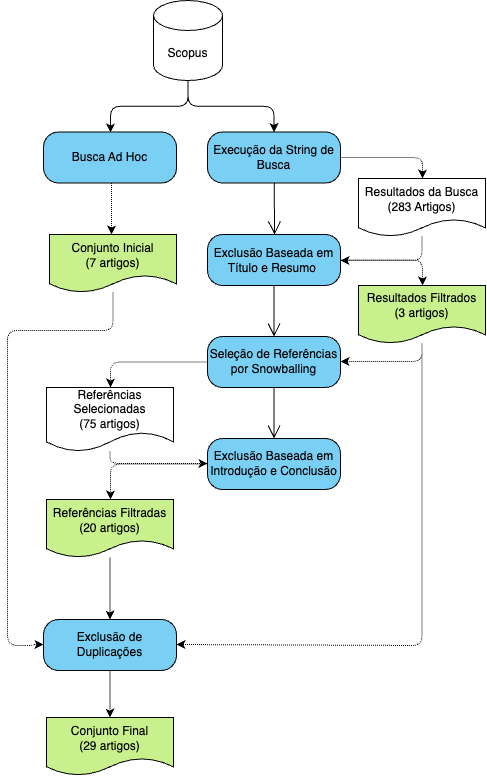
\includegraphics[width=0.7\linewidth]{figuras/selecao.png}
    \begin{center}
        \text{Fonte: Autor}
    \end{center}
    \label{fig:selecao}
\end{figure}

\begin{table}[]
    \caption{Conjunto Final de Artigos}
    
    \begin{tabular}{|p{.5cm}|p{6cm}|p{4cm}|p{4cm}|}
        \hline
        Nº & Título & Publicado em revista? & Referência \\ \hline
        1 & \textit{A New Framework for Online Testing of Heterogeneous Treatment Effect} & Não & \citeonline{yu_new_2020} \\ \hline
        2 & \textit{A/B testing: A Systematic Literature Review} & Sim & \citeonline{quin_b_2024} \\ \hline
        3 & \textit{An Activity and Metric Model for Online Controlled Experiments} & Não & \citeonline{kuhrmann_activity_2018} \\ \hline
        4 & \textit{An Infrastructure for Platform-Independent Experimentation of Software Changes} & Não & \citeonline{bures_infrastructure_2021} \\ \hline
        5 & \textit{Automatic Detection and Diagnosis of Invalid Online Experiments} & Não & \citeonline{chen_automatic_2018} \\ \hline
        6 & \textit{Characterization of Continuous Experimentation in Software Engineering: Expressions, Models and Strategies} & Sim & \citeonline{erthal_characterization_2023} \\ \hline
        7 & \textit{Characterizing Experimentation in Continuous Deployment: A Case Study on Bing} & Sim & \citeonline{kevic_characterizing_2017} \\ \hline
        8 & \textit{Enterprise-Level Controlled Experiments at Scale: Challenges and Solutions} & Não & \citeonline{liu_enterprise-level_2019} \\ \hline
        9 & \textit{From Opinions to Data-Driven Software R\&D: A Multi-case Study on How to Close the 'Open Loop' Problem} & Não & \citeonline{olsson_opinions_2014} \\ \hline
        10 & \textit{Hitting the target: Practices and Steps for moving toward innovation experiment systems} & Não & \citeonline{fernandes_hitting_2015} \\ \hline
        11 & \textit{Hypotheses Engineering: First Essential Steps of Experiment-Driven Software Development} & Não & \citeonline{melegati_hypotheses_2019} \\ \hline
        12 & \textit{Online Controlled Experiments at Large Scale} & Não & \citeonline{kohavi_online_2013} \\ \hline
        \multicolumn{4}{|c|}{Continua na Tabela \ref{tab:conjunto-final-2}} \\ \hline
    \end{tabular}
    
    \begin{center}
        \text{Fonte: Autor}
    \end{center}

    \label{tab:conjunto-final}
\end{table}

\begin{table}[]
    \caption{Continuação do Conjunto Final de Artigos}
    
    \begin{tabular}{|p{.5cm}|p{6cm}|p{4cm}|p{4cm}|}
        \hline
        \multicolumn{4}{|c|}{Continuação da Tabela \ref{tab:conjunto-final}} \\ \hline
        Nº & Título & Publicado em revista? & Referência \\ \hline
        13 & \textit{Seven Pitfalls to Avoid When Running Controlled Experiments on the Web} & Não & \citeonline{crook_seven_2009} \\ \hline
        14 & \textit{Statistical Challenges in Online Controlled Experiments: A Review of A/B Testing Methodology} & Sim & \citeonline{larsen_statistical_2024} \\ \hline
        15 & \textit{The Benefits of Controlled Experimentation at Scale} & Não & \citeonline{fabijan_benefits_2017} \\ \hline
        16 & \textit{The HURRIER process for experimentation in business-to-business mission-critical systems} & Sim & \citeonline{issa_mattos_hurrier_2023} \\ \hline
        17 & \textit{The Online Controlled Experiment Lifecycle} & Sim & \citeonline{fabijan_online_2020} \\ \hline
        18 & \textit{The RIGHT Model for Continuous Experimentation} & Sim & \citeonline{fagerholm_right_2017} \\ \hline
        19 & \textit{Three Key Checklists and Remedies for Trustworthy Analysis of Online Controlled Experiments at Scale} & Não & \citeonline{fabijan_three_2019} \\ \hline
        20 & \textit{Towards Automated A/B Testing} & Não & \citeonline{le_goues_towards_2014} \\ \hline
        21 & \textit{Towards Continuous Customer Validation: A Conceptual Model for Combining Qualitative Customer Feedback with Quantitative Customer Observation} & Não & \citeonline{olsson_towards_2015} \\ \hline
        22 & \textit{Towards Customer-centric Software Development: A Multiple-case Study} & Não & \citeonline{sauvola_towards_2015} \\ \hline
        23 & \textit{Understanding Hypotheses Engineering in Software Startups through a Gray Literature Review} & Sim & \citeonline{melegati_understanding_2021} \\ \hline
    \end{tabular}
    
    \begin{center}
        \text{Fonte: Autor}
    \end{center}

    \label{tab:conjunto-final-2}
\end{table}




\section{Resultados}
\label{sec:rsl-resultados}

Durante a leitura integral dos artigos selecionados, realizou-se a etapa final da revisão, a extração de dados. O formulário utilizado foi apresentado na Tabela \ref{tab:protocolo-busca} e o resultado consolidado dos dados está acessível \href{https://docs.google.com/spreadsheets/d/1LyB3fCxzzelQDfBpfCC4t2Z91LUd1-lA/edit?usp=sharing&ouid=105055060757466273844&rtpof=true&sd=true}{nesta planilha}, disponibilizada publicamente. Para além da extração de dados, nesta subseção são apresentados os resultados da revisão estruturada da literatura, descrevendo como o material responde às questões de pesquisa definidas e como estes resultados influenciam o processo sistematizado para a proposta de estudo de caso deste trabalho.

\subsection{Quais são os processos/modelos utilizados no desenvolvimento orientado a dados?}

Diferentes processos e modelos são apresentados na literatura e o escopo deles varia quanto ao que se propõem a sistematizar. Alguns tratam de atividades específicas da experimentação, já outros se propõem a esquematizar todo o processo de desenvolvimento, elencando papéis, atividades, artefatos etc. Há também aqueles que tratam do nível organizacional, especificando os passos que devem ser tomados para se adequar a cultura da empresa ao desenvolvimento orientado a dados.

Visando responder a questão de pesquisa, esta seção irá apresentar os modelos encontrados, os dividindo em categorias, explanando brevemente sobre as suas atividades e destacando quais deles influenciaram o pesquisador na construção da proposta desta monografia. Posteriormente, os principais modelos estudados para a proposta de estudo de caso serão destacadas, assim como suas determinadas influências.


\subsubsection{Modelos de Processo de Desenvolvimento}

\begin{itemize}

    \item \textbf{\textit{Combined Experimentation Process}:} O estudo de \citeonline{erthal_characterization_2023} busca caracterizar a literatura sobre Experimentação Contínua, oferecendo uma visão abrangente das principais atividades envolvidas na experimentação. Esse processo representa o principal resultado da revisão realizada pelos autores e visa discriminar atividades, fontes de informação e tomadas de decisão, separando o procedimento em três estágios \textit{build}, \textit{measure} e \textit{learn} (construção, metrificação e aprendizado), influenciado pela metodologia \textit{Lean Startup};
    
    \item \textbf{\textit{Hypex Model}:} Este modelo busca resolver o desafio identificado por \citeonline{olsson_opinions_2014}, denominado pelos autores como \textit{Open-loop Problem}, que se refere ao atraso entre os lançamentos de software e a avaliação por meio de processos de \textit{feedback}, dificultando a priorização de requisitos baseada em dados e tornando-a dependente de opiniões. O processo abrange diversas atividades, desde a construção do \textit{backlog}, passando pela priorização de funcionalidades, implementação e instrumentação, até a análise de dados. Além de delinear as atividades necessárias, os autores também discutem os desafios que motivaram a criação do modelo e as questões relacionadas à sua validação;
    
    \item \textbf{\textit{The RIGHT Model}:} Apresentado por \citeonline{fagerholm_right_2017}, o modelo também se baseia no ciclo \textit{Build-Measure-Learn} e busca integrar a visão de produto, estratégia de negócios e desenvolvimento de \textit{software} no processo de experimentação. O objetivo é unificar atividades como elicitação de requisitos, \textit{design}, implementação, testes, implantação e manutenção, utilizando os aprendizados obtidos nos experimentos. Além dessa proposta, os autores apresentam um estudo de caso múltiplo que forneceu os insumos necessários para consolidação do modelo e também discutem a infraestrutura necessária para sua implementação abordando papéis, ferramentas e artefatos;
    
    \item \textbf{\textit{The HURRIER Continuous Experimentation Process}:} Foi desenvolvido por \citeonline{issa_mattos_hurrier_2023} para sistemas B2B críticos, que exigem escalabilidade e inovação contínua, porém precisam mitigar os riscos o máximo possível. Envolve atividades de quatro áreas principais: \textit{R\&D} (Pesquisa e Desenvolvimento), validação interna, com um cliente e com múltiplos. Além disso, é uma abordagem flexível, que permite a utilização de partes separadas à depender do escopo do produto.
\end{itemize}
\subsubsection{Modelos de Evolução Organizacional}

\begin{itemize}
    
    \item \textbf{\textit{Stairway to Heaven Model}:} \citeonline{olsson2013towards} propõem um modelo que descreve um passo a passo composto de cinco etapas para empresas que desejam evoluir seus processos de trabalho. Foi desenvolvido visando guiar companhias que desejam evoluir as suas práticas de desenvolvimentos de \textit{software}. Um dos estudos selecionados através de \textit{snowballing}, \citeonline{fernandes_hitting_2015}, extende o modelo, utilizando dados coletados através de um estudo de caso. Os autores trazem práticas que caracterizam o passo a passo, dividas em quatro categorias: negócio, arquitetura, processo e organizacional; e
    
    \item \textbf{\textit{Experimentation Evolution Model}:} Visa apresentar um modelo de transição para uma empresa que trabalha apenas com opiniões e visa consolidar um processo de experimentação contínua. O modelo trata das diferentes fases que devem ser seguidas nessa evolução e as dividem em três dimensões: técnica, organizacional e negócios. Os autores descrevem cada fase e como se progredir em cada uma, falando sobre desafios e atividades \citeonline{fabijan_evolution_2017}.
    
\end{itemize}


\subsubsection{Modelos de Execução de Atividades Específicas}

\begin{itemize}
    
    \item \textbf{\textit{Hypotheses Engineering}:} Este processo foca na geração de hipóteses para a posterior validação por meio de experimentos. Os autores fazem um contraponto entre o desenvolvimento orientado a requisitos e do orientado a experimentos, apontando para a necessidade de um processo contínuo de geração e priorização de ideias. O processo é separado em quatro atividades, geração, documentação, análise e priorização \cite{melegati_hypotheses_2019}. Além da publicação citada, alguns dos autores realizaram uma posterior revisão de literatura cinza, visando entender como as atividades propostas no modelo são utilizadas na prática no mercado \cite{melegati_understanding_2021};

    \item \textbf{\textit{QCD Model}:} Visando unir dados quantitativos e qualitativos durante o processo de avaliação de funcionalidades, \citeonline{olsson_towards_2015} propõe o chamado \textit{Qualitative/quantitative Customer-driven Development}. O modelo trata os requisitos como hipóteses que devem ser avalidas junto aos clientes antes de se formalizar o que será desenvolvido, se formando um procedimento de validação contínua. O propósito é que seja executada uma rodada da chamada técnica \textit{Customer Feedback} antes da validação experimental, que consiste em observações, questionários e entrevistas para coleta de dados. Os autores advogam que esta fase pode facilitar o processo de experimentação, dado que não é necessária a implementação do \textit{software}, além de que os dados qualitativos podem ajudar a trazer sentido aos dados quantitativos;
    
    \item \textbf{\textit{Sequential Score Test}:} O \textit{framework} apresentado por \cite{yu_new_2020} foca na análise dos dados, e visa mitigar possíveis más práticas nos testes de hipóteses. Os autores advogam que para um teste de hipótese acontecer corretamente se deve definir o tamanho da amostra antes do período de teste e que efeitos heterogêneos devem ser observados, o que comumente não acontece no ritmo acelerado da indústria, o que pode gerar resultados enviesados. São propostas atividades de testes sequenciais que visam tratar destas lacunas;
    
    \item \textbf{\textit{The Online Controlled Experiment Lifecycle}:} O ciclo proposto por \citeonline{kohavi_online_2013} visa apresentar as etapas dos experimentos controlados \textit{online}, que são a ideação, o desenvolvimento e a análise. Os autores, além de caracterizar as etapas, descrevem suas atividades e mitigações de risco, visando prover uma visão geral sobre \textit{OCEs}. Embora seja um ciclo de vida, não apresenta um sistema que possa ser considerado um processo completo de desenvolvimento; e
    
    \item \textbf{\textit{Three Key Checklists for Trustworthy Analysis of OCEs}:} \citeonline{fabijan_three_2019} apresentam três conjuntos de listas de tarefas para servirem de guia na execução de experimentos. O propósito destas tarefas é garantir que os principais fatores que garantem o sucesso de um experimento sejam endereçados. Elas são separadas em três, uma para a parte da ideação, outra para a fase de execução e a última para o momento da análise.
    
    
\end{itemize}

Após conhecer os modelos existentes na literatura, optou-se por utilizar do modelo proposto por \citeonline{erthal_characterization_2023}, o \textit{Combined Experimentation Process}, como base para a proposta deste trabalho.

Além disso, também foi escolhido o modelo de Engenharia de Hipóteses, apresentado por \citeonline{melegati_hypotheses_2019}. Este material servirá de apoio para a realização da atividade de ideação e formulação de hipóteses que precede a execução dos experimentos.

Outro modelo que deve servir de guia para a execução das atividades é a lista de tarefas apresentada por \citeonline{fabijan_three_2019}. As três \textit{checklists} que o artigo apresenta são de grande contribuição para a construção de um \textit{guideline} para a execução de experimentos. O propósito é utilizar da influência do modelo para criar uma lista de tarefas similar que possa ser utilizada no contexto do produto investigado.



\subsection{Quais são as estratégias utilizadas no desenvolvimento orientado a dados?}

O tipo de estratégia mais comum encontrada é o Teste A/B, também chamado de OCE (ou \textit{Online Controlled Experiment}), foi citado por todos os artigos lidos. Existem algumas variações desse teste, como, por exemplo, o MVP ou MVF (\textit{Minimal Viable Product} ou \textit{Minimal Viable Feature}), onde a versão mais simples possível da nova funcionalidade é desenvolvida e testada para gerar aprendizados que possam orientar o desenvolvimento da versão completa \cite{fabijan_online_2020} \cite{chen_understanding_2024} \cite{kohavi_online_2013} \cite{fagerholm_right_2017} \cite{sauvola_towards_2015} \cite{melegati_hypotheses_2019} \cite{kuhrmann_activity_2018}.

Além disso, há estratégias que visam gerar aprendizados em vez de apenas validar novas funcionalidades. Nesse contexto, temos os Testes A/A, que coletam dados de duas populações utilizando a mesma versão do \textit{software} para estudar o comportamento dos usuários \cite{fabijan_evolution_2017} \cite{fabijan_three_2019} \cite{kuhrmann_activity_2018} \cite{crook_seven_2009} \cite{fabijan_benefits_2017}. Também existem os Experimentos Reversos, onde funcionalidades aparentemente obsoletas são removidas, diminuindo a complexidade do código, e as métricas observadas buscam garantir que não houve impacto negativo para o usuário \cite{fabijan_benefits_2017}. Outros exemplos incluem testes negativos, experimentos de calibração/otimização, entre outros \cite{kohavi_online_2013} \cite{issa_mattos_hurrier_2023}.

Outro tipo de estratégia refere-se ao tipo de \textit{release} que será realizado pela empresa, visando minimizar o risco de entregas que possam causar danos ao usuário. Alguns exemplos são \textit{canary releases}, \textit{dark launches}, \textit{gradual rollouts}, entre outros \cite{chen_understanding_2024} \cite{issa_mattos_hurrier_2023} \cite{bures_infrastructure_2021}.

\subsection{Quais ferramentas/tecnologias comumente utilizadas na indústria para instrumentalização de experimentos?}

Com relação a ferramentas existentes no mercado, nesta revisão estruturada da literatura foram identificadas poucas opções, já que os artigos selecionados focaram na definição de um processo e descrição das atividades a serem realizadas. Entretanto houveram algumas citações a tecnologias, as mesmas são apresentadas na Tabela \ref{tab:rsl-ferramentas}.

\begin{table}[]
\centering
    \caption{Ferramentas Citadas na Literatura}

    \begin{tabular}{|p{2cm}|p{3cm}|p{9cm}|}
        \hline
        \textbf{Tecnologia} & \textbf{Citado por} & \textbf{Descrição} \\ \hline
        Analytics Experimentation Platform & \citeonline{kevic_characterizing_2017}. & Criada pela Google para realização de testes A/B integrados ao Google Analytics com segmentação de público. Foi descontinuada em 2024 \cite{analytics_experimentation_framework}. \\ \hline
        Maxymiser & \citeonline{fabijan_evolution_2017}. & Criada para a realização de testes A/B e também multivariáveis, permite analisar o comportamento dos usuários em tempo real. Solução proprietária da Oracle que foi descontinuada em 2020 \cite{maxymiser}. \\ \hline
        Mixpanel & \citeonline{fabijan_evolution_2017}. & Plataforma de análise e engajamento que facilita o rastreamento e a compreensão do comportamento dos usuários em aplicações \textit{web} e \textit{mobile}. Dentre outras funcionalidades, permite a análise detalhada de eventos, a segmentação de usuários e a criação de funis de conversão, além de uma API robusta para personalização e automação. Solução proprietária que oferece modelos sob assinatura com uma opção de plano gratuito \cite{mixpanel2024}. \\ \hline
        Optimizely & \citeonline{fabijan_evolution_2017}, \citeonline{kohavi_online_2013} e \citeonline{bures_infrastructure_2021}. & Esta ferramenta, dentre outras funcionalidades, permite a criação de testes A/B para otimizar interfaces. Oferece um editor visual para criação de experimentos sem código. Permite testar aplicações \textit{web} e \textit{mobile}. Solução proprietária que oferece modelos sob assinatura.\cite{optimizely}. \\ \hline
        PlanOut & \citeonline{kevic_characterizing_2017}. & O PlanOut é uma plataforma de código aberto criada pelo Facebook para facilitar a execução e iteração de experimentos complexos. Oferece uma implementação em Python, além de versões para outras linguagens, como Java, JavaScript e PHP. Inclui classes extensíveis para definir experimentos e um interpretador para executar \textit{scripts}. A última atualização pública do repositório foi no ano de 2020, tendo sido arquivado pela empresa em 2021, cerca de 3 anos antes do desenvolvimento desta monografia \cite{planout}. \\ \hline
        Wasabi & \citeonline{kohavi_online_2013}. & Plataforma de código livre para realização de experimentos controlados em larga escala. Permite controlar os próprios dados, realizar testes em plataformas \textit{web}, \textit{mobile} e \textit{desktop} e gerir experimentos através de uma interface de gestão. A última atualização no repositório público foi em Agosto de 2019, 5 anos antes do desenvolvimento desta monografia \cite{wasabi}. \\ \hline
        \multicolumn{3}{|c|}{Continua na Tabela \ref{tab:rsl-ferramentas-2}} \\ \hline
    \end{tabular}

    \label{tab:rsl-ferramentas}
    
    \begin{center}
        \text Fonte: Autor
    \end{center}
\end{table}

\begin{table}[]
\centering
    \caption{Continuação das Ferramentas Citadas na Literatura}

    \begin{tabular}{|p{2cm}|p{3cm}|p{9cm}|}
        \hline
        \multicolumn{3}{|c|}{Continuação da Tabela \ref{tab:rsl-ferramentas}} \\ \hline
        \textbf{Tecnologia} & \textbf{Citado por} & \textbf{Descrição} \\ \hline
        XLNT & \citeonline{kevic_characterizing_2017}. & Foi desenvolvido para atender as necessidades específicas do \textit{LinkedIn} e segue como produto exclusivo da empresa. Permite a criação de testes A/B e multivariados com foco em personalização de experiências. A plataforma oferece uma interface de gestão para o controle e análise de experimentos, permitindo a execução simultânea de múltiplos testes.  \cite{xlnt}. \\ \hline
        \multicolumn{3}{|c|}{Continua na Tabela \ref{tab:conjunto-final-2}} \\ \hline
    \end{tabular}

    \label{tab:rsl-ferramentas-2}
    
    \begin{center}
        \text Fonte: Autor
    \end{center}
\end{table}

\subsection{Quais os principais desafios e problemas reportados?}

A literatura relata desafios referentes à velocidade de desenvolvimento e são citados a necessidade de sistematização de um processo de desenvolvimento e da coleta dos dados com uma plataforma sólida, fatores que demandam tempo e esforço. Ainda relacionado ao tempo desprendido neste processo, alguns estudos relatam desafios em escalar o processo pela dificuldade de automatizar determinadas atividades, como a geração das hipóteses, \textit{design}, a análise dos dados e execução dos experimentos \cite{erthal_characterization_2023} \cite{fabijan_evolution_2017}  \cite{sauvola_towards_2015} \cite{quin_b_2024} \cite{fernandes_hitting_2015} \cite{fagerholm_right_2017} \cite{kevic_characterizing_2017} \cite{kohavi_online_2013} \cite{bures_infrastructure_2021} \cite{liu_enterprise-level_2019} \cite{chen_automatic_2018} \cite{fabijan_online_2020} \cite{le_goues_towards_2014}.

Em alguns estudos são relatadas dificuldades em trabalhar com as métricas de uso, tanto pela dificuldade de escolher as variáveis corretas quanto para realizar uma análise confiável destes dados. Alguns exemplos de fatores que causam estes problemas são: a dificuldade de traduzir \textit{feedbacks} dos usuários para hipóteses testáveis; inexperiência da equipe com dados e a falta de tempo para realização de todas as atividades necessárias. Esses problemas podem acarretar experimentos mal desenhados e falsos positivos/negativos \cite{quin_b_2024} \cite{erthal_characterization_2023} \cite{issa_mattos_hurrier_2023} \cite{fabijan_evolution_2017} \cite{fernandes_hitting_2015} \cite{fabijan_three_2019} \cite{kuhrmann_activity_2018} \cite{fagerholm_right_2017} \cite{olsson_towards_2015} \cite{kevic_characterizing_2017} \cite{crook_seven_2009} \cite{kohavi_online_2013} \cite{yu_new_2020} \cite{liu_enterprise-level_2019} \cite{kohavi_online_2013} \cite{fabijan_benefits_2017} \cite{le_goues_towards_2014} \cite{larsen_statistical_2024}. Alguns estudos focam nestes tipos de desafios, trazendo conhecimento e propondo atividades para mitigação de riscos \cite{kohavi_seven_2014} \cite{larsen_statistical_2024}.



\section{Resumo do capítulo}

Este capítulo apresentou como foi realizado o processo de revisão da literatura, baseado no protocolo proposto por \citeonline{kitchenham_rsl}. Foram detalhados o planejamento, a estruturação do protoloco e a construção da \textit{string} de busca, seguidos pela apresentação dos resultados, tanto da busca, quanto do processo de \textit{snowballing}. Em linhas gerais, foi apresentada a Tabela \ref{tab:conjunto-final} e a Figura \ref{fig:selecao}, que trazem o conjunto final de artigos selecionados para leitura integral e o processo de seleção. Além disso, são apresentados os resultados da leitura completa do material, descrevendo como a literatura respondeu às questões de pesquisa desta revisão estruturada.


\chapter{Proposta de Estudo de Caso}
\label{ch:proposta}

Neste capítulo é apresentado o planejamento da fase de observação e experimentação desta pesquisa, objeto da segunda fase deste Trabalho de Conclusão de Curso.

\section{Definição}

Um Estudo de Caso é um método de investigação que visa analisar um fenômeno em seu contexto real e contemporâneo. Diferentes fontes de dados e técnicas podem ser utilizadas para essa abordagem, como pesquisas bibliográficas, entrevistas e observações \cite{wohlin_experimentation_2012}. \citeonline{yin_case_study_2009} ressalta que esse método parte do pressuposto de que um fenômeno de interesse não é separável de seu contexto.

Costuma ser aplicado na Engenharia de Software quando se busca compreender um fenômeno em seu contexto real. O principal objetivo de um Estudo de Caso é coletar e analisar dados, a fim de realizar inferências que possam auxiliar no estabelecimento de relações entre os objetos de estudo \cite{wohlin_experimentation_2012}.


\subsection{Objetivo}

A literatura indica que priorizar funcionalidades para desenvolvimento com base apenas em opiniões pode resultar em um desalinhamento com o que realmente agrega valor ao usuário e ao negócio. Nesse contexto, as empresas tem buscado a investigação experimental para assegurar a tomada de decisão e a avaliação da qualidade de uso de seu \textit{software} baseadas em evidências \cite{olsson_opinions_2014}. No entanto, sistematizar um processo de experimentação é complexo e requer esforço organizacional não apenas no nível tecnológico, mas também nos níveis culturais e de negócios \cite{fabijan_evolution_2017}. Dessa forma, o presente estudo visa investigar como a adoção de práticas de experimentação contínua pode auxiliar na tomada de decisões estratégicas e na análise da qualidade em uso de um \textit{software}.


\subsection{Caso}

O objeto de estudo desta investigação é um produto de \textit{software} desenvolvido por uma empresa privada brasileira, que oferece uma solução de ambiente virtual de aprendizagem. Este \textit{SaaS} é utilizado por cerca de quinhentas escolas brasileiras e atende a uma base de aproximadamente 100 mil usuários. A plataforma possui um código-base com cerca de 740 mil linhas.

O produto se trata de uma plataforma \textit{web} escrita em \textit{TypeScript}, uma linguagem de programação derivada do \textit{JavaScript}. Hoje, é mantido por cerca de 30 desenvolvedores, de diferentes níveis de experiência, divididos em 5 equipes que também possuem outros profissionais, como \textit{designers}, gerentes, consultores de negócio e analistas de qualidade.

O produto foi selecionado por seu desenvolvimento obedecer a cadência de desenvolvimento contínuo, o que viabiliza a implantação de um processo de Experimentação Contínua. Outro fator importante é a larga população de usuários que, permitirá a definição de amostras com significância estatística, aumentando a confiabilidade das análises estatísticas. Por fim, a empresa demonstrou disposição em colaborar com a pesquisa, o que também possibilita a coleta de dados sob a perspectiva dos colaboradores envolvidos.


\subsection{Trabalhos Relacionados}

Durante a revisão da literatura, descrita no Capítulo \ref{ch:revisao}, foram selecionados estudos que pudessem servir de insumo para a construção desta monografia.

A principal influência deste trabalho foi o estudo de \citeonline{erthal_characterization_2023}, que realizou uma caracterização do estado da arte do desenvolvimento orientado a dados e propôs um processo combinado baseado nos modelos e práticas encontrados em sua revisão da literatura. Com base neste modelo, foi mapeado o atual processo de desenvolvimento do projeto analisado, para elencar as atividades necessárias para esquematizar um sistema de experimentação contínua.

O trabalho de \citeonline{melegati_understanding_2021} apresenta a chamada \textit{Hypotheses Engineering} e suas práticas, trazendo uma revisão da literatura cinza para descrever como essas práticas são utilizadas no mercado. A engenharia de hipóteses, proposta por \citeonline{melegati_hypotheses_2019}, descreve as atividades necessárias para a formalização de hipóteses, etapa essencial para a realização de experimentos que validam as suposições dos responsáveis pelo desenvolvimento do produto.

Já o estudo de \cite{fabijan_three_2019} traz \textit{checklists} em forma de listas de verificação, com três listas que servem de guia para a execução de experimentos controlados: uma na fase de \textit{design} do experimento, outra na sua execução, e uma terceira na etapa de análise de dados. O propósito é listar atividades que garantam a execução apropriada do experimento e uma tomada de decisão confiável.

Outros modelos que visam à sistematização do processo em sua totalidade ou à descrição de atividades específicas também foram encontrados \cite{fagerholm_right_2017, issa_mattos_hurrier_2023, olsson_opinions_2014}. Além disso, na literatura há estudos de caso realizados em diferentes orgnizaçõe, mapeamentos e revisões que, semelhantes a esta monografia, buscam avaliar a experimentação e compreender suas práticas, benefícios e desafios \cite{kevic_characterizing_2017, kuhrmann_activity_2018, fernandes_hitting_2015, sauvola_towards_2015, issa_mattos_hurrier_2023, kohavi_online_2013, fabijan_benefits_2017, quin_b_2024, erthal_characterization_2023, larsen_statistical_2024}. Embora nem todos os artigos citados sejam influências diretas no processo proposto, suas leituras foram essenciais para a compreensão das atividades a serem realizadas neste trabalho.

Outros estudos focam em descrever os desafios da experimentação contínua, ajudando a desenhar um processo mais robusto e análises com maior acurácia. O trabalho de \citeonline{larsen_statistical_2024} destaca desafios estatísticos na realização de experimentos; um exemplo particularmente relevante para o contexto deste estudo é o chamado \textit{optional stopping}, que envolve monitorar as métricas durante a execução do experimento para interromper o processo se necessário. Esse processo é crucial para detectar, antes da liberação de uma \textit{release}, se uma alteração prejudica o usuário. Para mitigar esse risco, o estudo propõe a liberação gradativa das mudanças.

Ainda nesse contexto, o trabalho de \citeonline{crook_seven_2009} identifica armadilhas comuns, como a validação do \textit{design} experimental. Os autores enfatizam a importância dessa etapa para garantir a qualidade do teste e sugerem que, antes do desenvolvimento, o experimento seja validado através da coleta de dados de uso antes mesmo da construção da nova versão para avaliação de padrões inesperados, para assegurar que as versões corretas serão atribuídas aos usuários e que o comportamento das populações estão alinhadas e seguindo o esperado.

Neste estudo, inicialmente serão formalizadas hipóteses a partir de diferentes insumos, como \textit{feedback} de clientes, estado do mercado e conhecimento de negócio. Após a formalização, documentação e priorização das hipóteses, uma será escolhida para avaliação. Antes do desenvolvimento, será preparada a coleta de dados, com a definição das métricas de uso a serem observadas durante o período da execução do experimento. Além disso, será realizado um pré-estudo para avaliar o \textit{design} do experimento.

Com as métricas definidas, a nova versão do produto será desenvolvida e lançada para um grupo selecionado de usuários, e os dados começarão a ser coletados. Por fim, a partir dessa coleta, os dados serão analisados e testes estatísticos serão realizados para verificar se há uma diferença significativa entre as versões. Essa análise determinará se a hipótese é confirmada e a nova versão deve ser liberada para todos os usuários, ou se o tratamento não se sustenta e deve ser abandonado.


\subsection{Questão de Pesquisa}

Buscando responder à questão principal de pesquisa do trabalho, apresentada na Seção \ref{sec:questao} (Como a adoção de práticas de experimentação contínua pode auxiliar a tomada de decisão sobre a implantação de novas versões de um produto de software web?), foram derivadas questões específicas para o estudo de caso, juntamente com as métricas que serão utilizadas para sua avaliação, seguindo a abordagem GQM. Essas questões e métricas são apresentadas a seguir.

\begin{itemize}
    \item \textbf{Questão Específica 1:} Durante o experimento controlado, foi possível identificar diferenças significativas nas métricas de uso escolhidas para avaliar a hipótese?

    \begin{itemize}
        \item \textbf{Métrica 1.1:} Diferença estatística entre as distribuições de dados das versões de controle e tratamento. A métrica específica depende da hipótese a ser testada, que será definida inicialmente, antes do desenvolvimento da nova versão. Uma vez definida a funcionalidade, as métricas serão escolhidas para refletir o comportamento dos usuários durante o uso do produto e dizer qual versão se desempenha melhor. 
    \end{itemize}
    
    \item \textbf{Questão Específica 2:} Foi possível rejeitar a hipótese nula e aceitar a versão de tratamento como superior?

    \begin{itemize}
        \item \textbf{Métrica 2.1:} Diferença nas médias dos valores observados nos dois conjuntos de dados, de tratamento e de controle.
    \end{itemize}
  
    \item \textbf{Questão Específica 3:} O processo de experimentação contribuiu para uma tomada de decisão baseada em dados?

    \begin{itemize}
        \item \textbf{Métrica 3.1:} Se as atividades pretendidas conseguiram ser realizadas em sua completude.
    \end{itemize}

    \begin{itemize}
        \item \textbf{Métrica 3.2:} Opinião dos colaboradores envolvidos em relação ao nível de contribuição do processo aplicado na tomada de decisão.
    \end{itemize}

    \begin{itemize}
        \item \textbf{Métrica 3.2:} Opiniões qualitativas dos colaboradores envolvidos em relação ao processo aplicado de modo geral.
    \end{itemize}
    
\end{itemize}

\subsection{Fonte de Dados}

A fonte de dados quantitativos será o uso da plataforma pelos usuários. Uma vez que o \textit{software} esteja preparado para coletar os dados de uso da plataforma, assim que os usuários utilizarem a funcionalidade testada, métricas relacionadas ao seu uso serão coletadas como, por exemplo, tempo de uso, quantidade de cliques.

Como a funcionalidade implementada será apresentada em duas versões diferentes, espera-se que os dados coletados sejam significativamente distintos entre as duas populações de usuários. Esses dados devem ser suficientes para uma análise estatística que irá determinar qual versão é mais adequada para os clientes.

Além disso, a opinião dos colaboradores envolvidos no processo também será coletada, através de formulários de opinião, como uma fonte adicional de dados, visando entender se a metodologia ajudou na tomada de decisões e se houve uma evolução percebida em comparação ao processo existente na empresa.


\section{Procedimentos}
\label{sec:procedimentos}

Neste trabalho foi proposto um processo que deve guiar o desenvolvimento durante a execução deste estudo de caso. A partir da revisão da literatura descrita em \ref{ch:revisao}, procurou-se compreender as atividades envolvidas na experimentação continua e encontrar modelos ou processos já existentes na literatura. 

Em seguida, buscou se analisar o processo atual da empresa, compreendendo as atividades já existentes e realizadas pelos desenvolvedores do produto para posterior definição de atividades que viabilizariam a execução de experimentos controlados. Esta formalização se baseou principalmente no modelo \textit{Combined Process for Experimentation}, proposto por \citeonline{erthal_characterization_2023} e já apresentado na Figura \ref{fig:erthal-process}.

Feita essa formalização, através dos insumos encontrados na literatura, foi proposto um novo processo, visando a introdução de práticas de experimentação contínua e que servirá de objeto de estudo desta monografia. A versão inicial, que ilustra o processo de desenvolvimento atualmente utilizado pela empresa, é apresentado na Figura \ref{fig:processo-atual}. Já o processo proposto neste trabalho, adaptado a partir do atual, é apresentada na Figura \ref{fig:processo-novo}, onde os itens destacados de vermelho são as novas atividades e artefatos, trazendo o fluxo que deve ser seguido nesta investigação.

Para a coleta de dados referentes aos resultados das atividades realizadas e como o processo proposto se desempenhou, serão realizados questionários, que devem ser respondidos pelos colaboradores participantes. Já os dados de segunda ordem, ou seja, aqueles coletados por meio de observações, serão as métricas e medidas de qualidade em uso definidas durante a ideação da hipótese a ser testada pelo experimento que será realizado.


\begin{figure}
    \centering
    \caption{Modelo do Fluxo de Atividades Atual do Produto Investigado}
    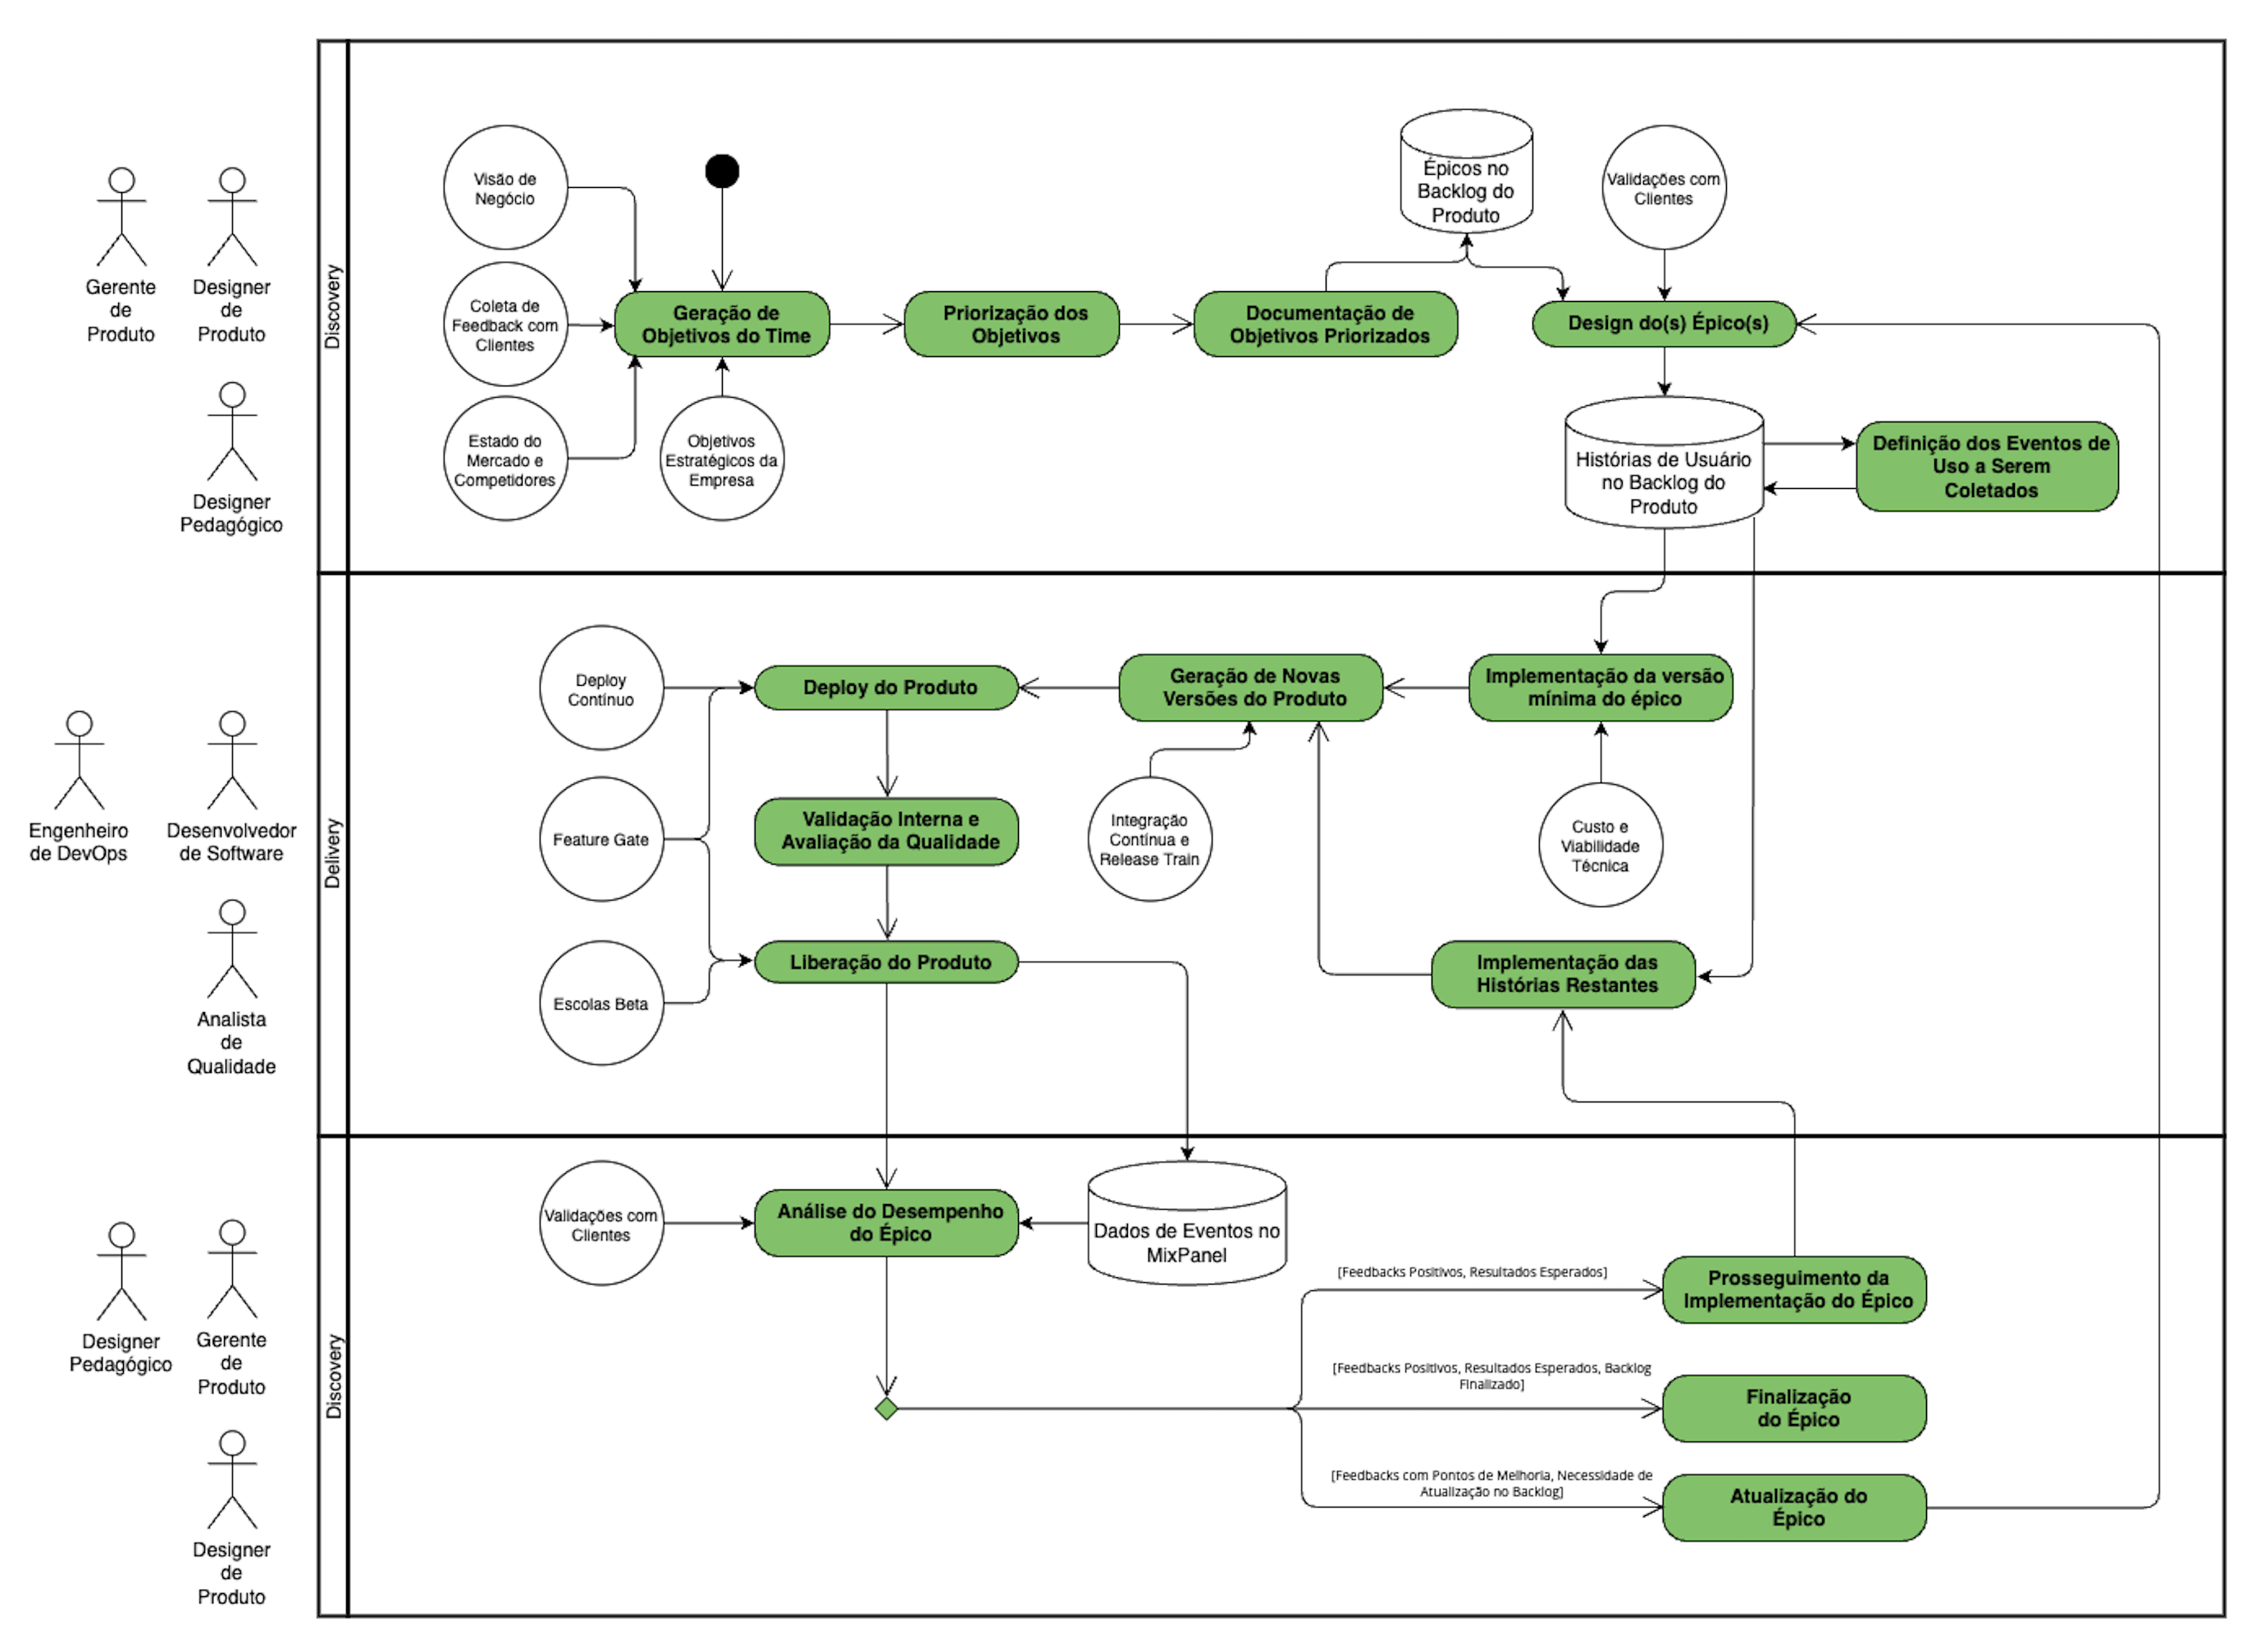
\includegraphics[width=1\linewidth]{figuras/processo-atual.png}
    \begin{center}
        \text{Fonte: Autor}
    \end{center}
    \label{fig:processo-atual}
\end{figure}

\begin{figure}
    \centering
    \caption{Modelo Proposto Para Implementação da Experimentação Contínua}
    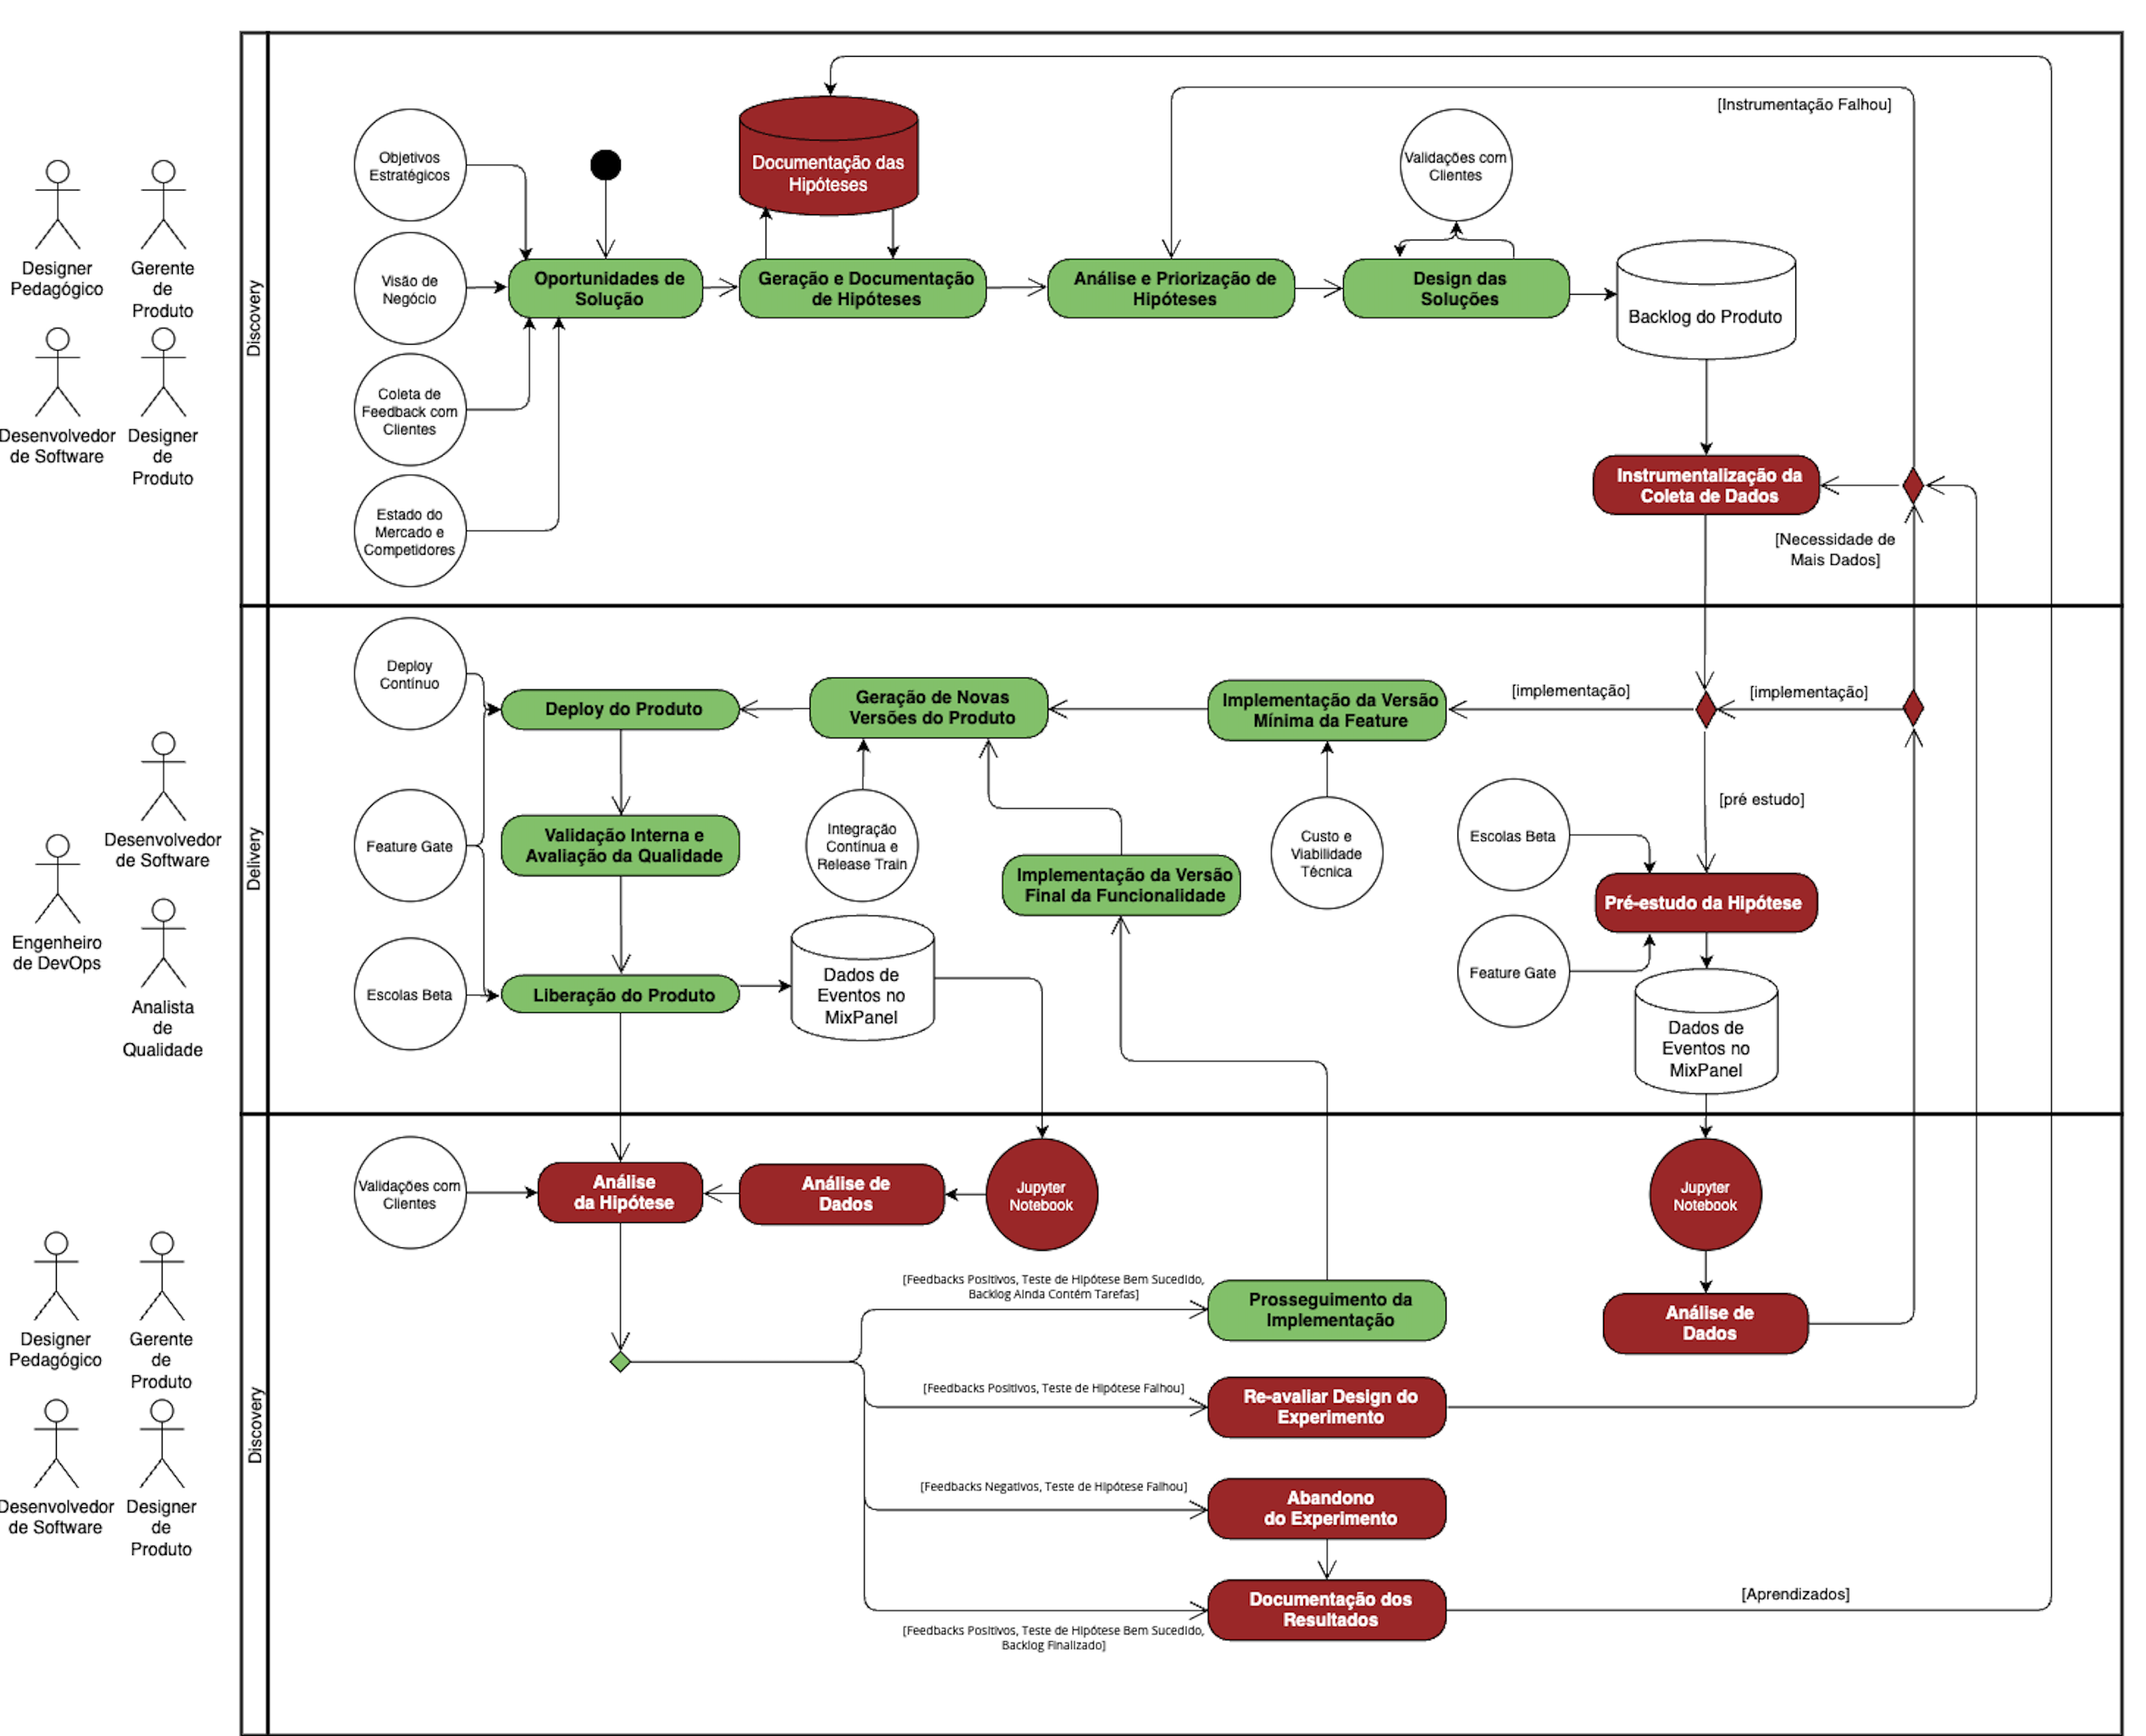
\includegraphics[width=1\linewidth]{figuras/processo-novo.png}
    \begin{center}
        \text{Fonte: Autor}
    \end{center}
    \label{fig:processo-novo}
\end{figure}


\subsection{Processo Proposto}
\label{subsec:fluxo}

Aqui serão descritas as atividades, fases, papeis e artefatos do processo proposto. Determinadas atividades do processo são iterativas e devem/podem ser realizadas novamente caso necessário. Abaixo são descritas as atividades a serem realizadas, conforme apresentado na Figura \ref{fig:processo-novo}.

\begin{itemize}
    \item \textbf{Documentação de Hipóteses:} Serão realizadas as atividades da Engenharia de Hipóteses, quer sejam: gerar; documentar; analisar e priorizar as suposições do time. O objetivo é formalizar as suposições em hipóteses para realização de testes estatísticos;
    
    \item \textbf{\textit{Design} do Experimento:} Serão criados os protótipos da hipótese selecionada para desenvolvimento, como já acontece hoje com as funcionalidades da empresa. A diferença é que também serão elencadas métricas do comportamento em uso que devem ser coletadas para avaliação da funcionalidade.

    \item \textbf{Instrumentalização da Coleta de Dados:} O ambiente de coleta de métricas e medidas será preparado; Antes do desenvolvimento efetivo da versão de tratamento, os eventos de uso necessários serão adicionados no código-fonte, separando as populações através de \textit{feature flags}.

    \item \textbf{Pré Estudo da Hipótese:} Antes da implementação e com a coleta de dados instrumentalizada, será feito um Teste A/A: ambas as populações serão expostas à versão de controle. O propósito é que o \textit{design} do experimento seja avaliado e a equipe retorne ao processo de instrumentalização ou análise da hipótese caso seja necessário.

    \item \textbf{Desenvolvimento do Tratamento:} A nova versão deve ser desenvolvida conforme planejado e liberada para os usuários selecionados.

    \item \textbf{Análise de Dados:} A partir das métricas coletadas serão realizados testes estatísticos de hipótese que devem ditar a implantação ou abandono da hipótese testada.

    \item \textbf{Coleta de Opinião:} Após a tomada de decisão referente ao experimento, será coletada a opinião dos colaboradores envolvidos referente ao desempenho do processo empregado.
\end{itemize}




\subsection{Atribuição das Variantes}

Para realizar a coleta de dados sobre o uso das diferentes versões do produto, ambas precisam ser distribuídas e apresentadas de maneira consistente aos clientes, a fim de observar como elas se comportam no mesmo período de tempo. Para isso, será utilizada a técnica de \textit{Feature Toggle}, descrita na Seção \ref{sec:ref-feature-toggle}.

Por se tratar de uma condicional no código, essa técnica permite que a distribuição das versões ocorra no lado do cliente, durante o uso do \textit{software}. Isso elimina certas camadas de complexidade, como a necessidade de liberar diferentes \textit{deploys}, o que exigiria uma nova configuração na infraestrutura do produto.

No caso do produto observado nesta pesquisa, a utilização dessa abordagem de desenvolvimento já é um padrão na empresa. Sendo assim, todas as funcionalidades desenvolvidas, são atreladas a \textit{feature gates}, que são ligados apenas para determinadas populações de usuários, a fim de se realizarem testes e coletas de \textit{feedbacks} qualitativos. Por isso, a companhia já possui diversas estratégias para lidar com esses \textit{toggles} e com a dívida técnica que eles acarretam:

\begin{itemize} 

    \item \textbf{Gerenciamento:} uma plataforma \textit{web} desenvolvida pela própria companhia é utilizada para gerenciar todas as \textit{flags}, bem como sua ativação. A interface amigável permite que até mesmo pessoas não desenvolvedoras sejam capazes de ativar ou desativar \textit{toggles}, além de entender quais estão ligadas ou não, e para quais usuários;
    
    \item \textbf{Persistência:} o produto consome o serviço de gerenciamento no momento da autenticação do usuário e preenche o estado da aplicação com as \textit{flags} ativadas para ele. Isso garante que, durante o uso, a consistência seja mantida e todos os fluxos sejam persistentes;
    
    \item \textbf{\textit{Backlog}:} durante a criação de tarefas para preenchimento do \textit{backlog}, caso alguma \textit{flag} esteja envolvida no desenvolvimento, também são adicionadas tarefas para sua remoção. Esta atividade, por sua vez, é despriorizada, mas mantida no \textit{backlog}, sendo executada apenas quando a funcionalidade já foi liberada para todos os usuários; e 
    
    \item \textbf{Automação:} um \textit{script} periódico é executado para buscar \textit{toggles} que não estejam mais sendo utilizados em nenhuma parte da base de código. O relatório final é analisado pelo time de engenharia, e as \textit{flags} a serem removidas são repassadas para suas respectivas equipes responsáveis. Isso garante que, mesmo que a remoção tenha sido esquecida durante a construção ou execução do \textit{backlog}, o time responsável seja relembrado de sua dívida técnica. 

\end{itemize}

Além do aparato técnico para divisão das versões, a empresa também possui mecanismos de negócio para tal. É oferecido, para clientes que já têm um bom relacionamento com a companhia, um modelo contratual de cliente beta, no qual a organização de ensino recebe novas funcionalidades antecipadamente, ciente de que estas ainda estão em fase experimental. Hoje, essas escolas representam cerca de 10\% da base de usuários (aproximadamente 10 mil pessoas).

Esse modelo permite a realização de testes com versões ainda em desenvolvimento, com processos de coleta de \textit{feedback} junto a docentes que se dispõem a participar de validações com a empresa. Dado esse contexto organizacional, optou-se por utilizar todos os aparatos já existentes para a realização do experimento, visando facilitar a implantação do processo proposto e reduzir sua complexidade.

Inicialmente, será definida uma \textit{feature flag} para representar o experimento, que será ativada para os usuários beta no momento da liberação da versão de tratamento, marcando o início da coleta de dados. A remoção do \textit{toggle} será realizada, juntamente com a do código-fonte a ser descartado, após a decisão sobre a versão que será implantada definitivamente.

A utilização de \textit{feature toggles} no contexto do experimento deste trabalho é exemplificada na Figura \ref{fig:toggle}. No exemplo há um componente chamado \textit{SomeComponent} e o mesmo utiliza da função \textit{useFeature} para verificar qual versão deve retornar, o controle ou o tratamento. A função \textit{useFeature}, por sua vez, possui a lista de \textit{flags} ativadas para o usuário, proveniente de uma solicitação prévia para o serviço de gerência de \textit{toggles}.


\begin{figure}
    \centering
    \caption{Exemplo de Utilização de \textit{Feature Toggles} Para Atribuição de Variantes}
    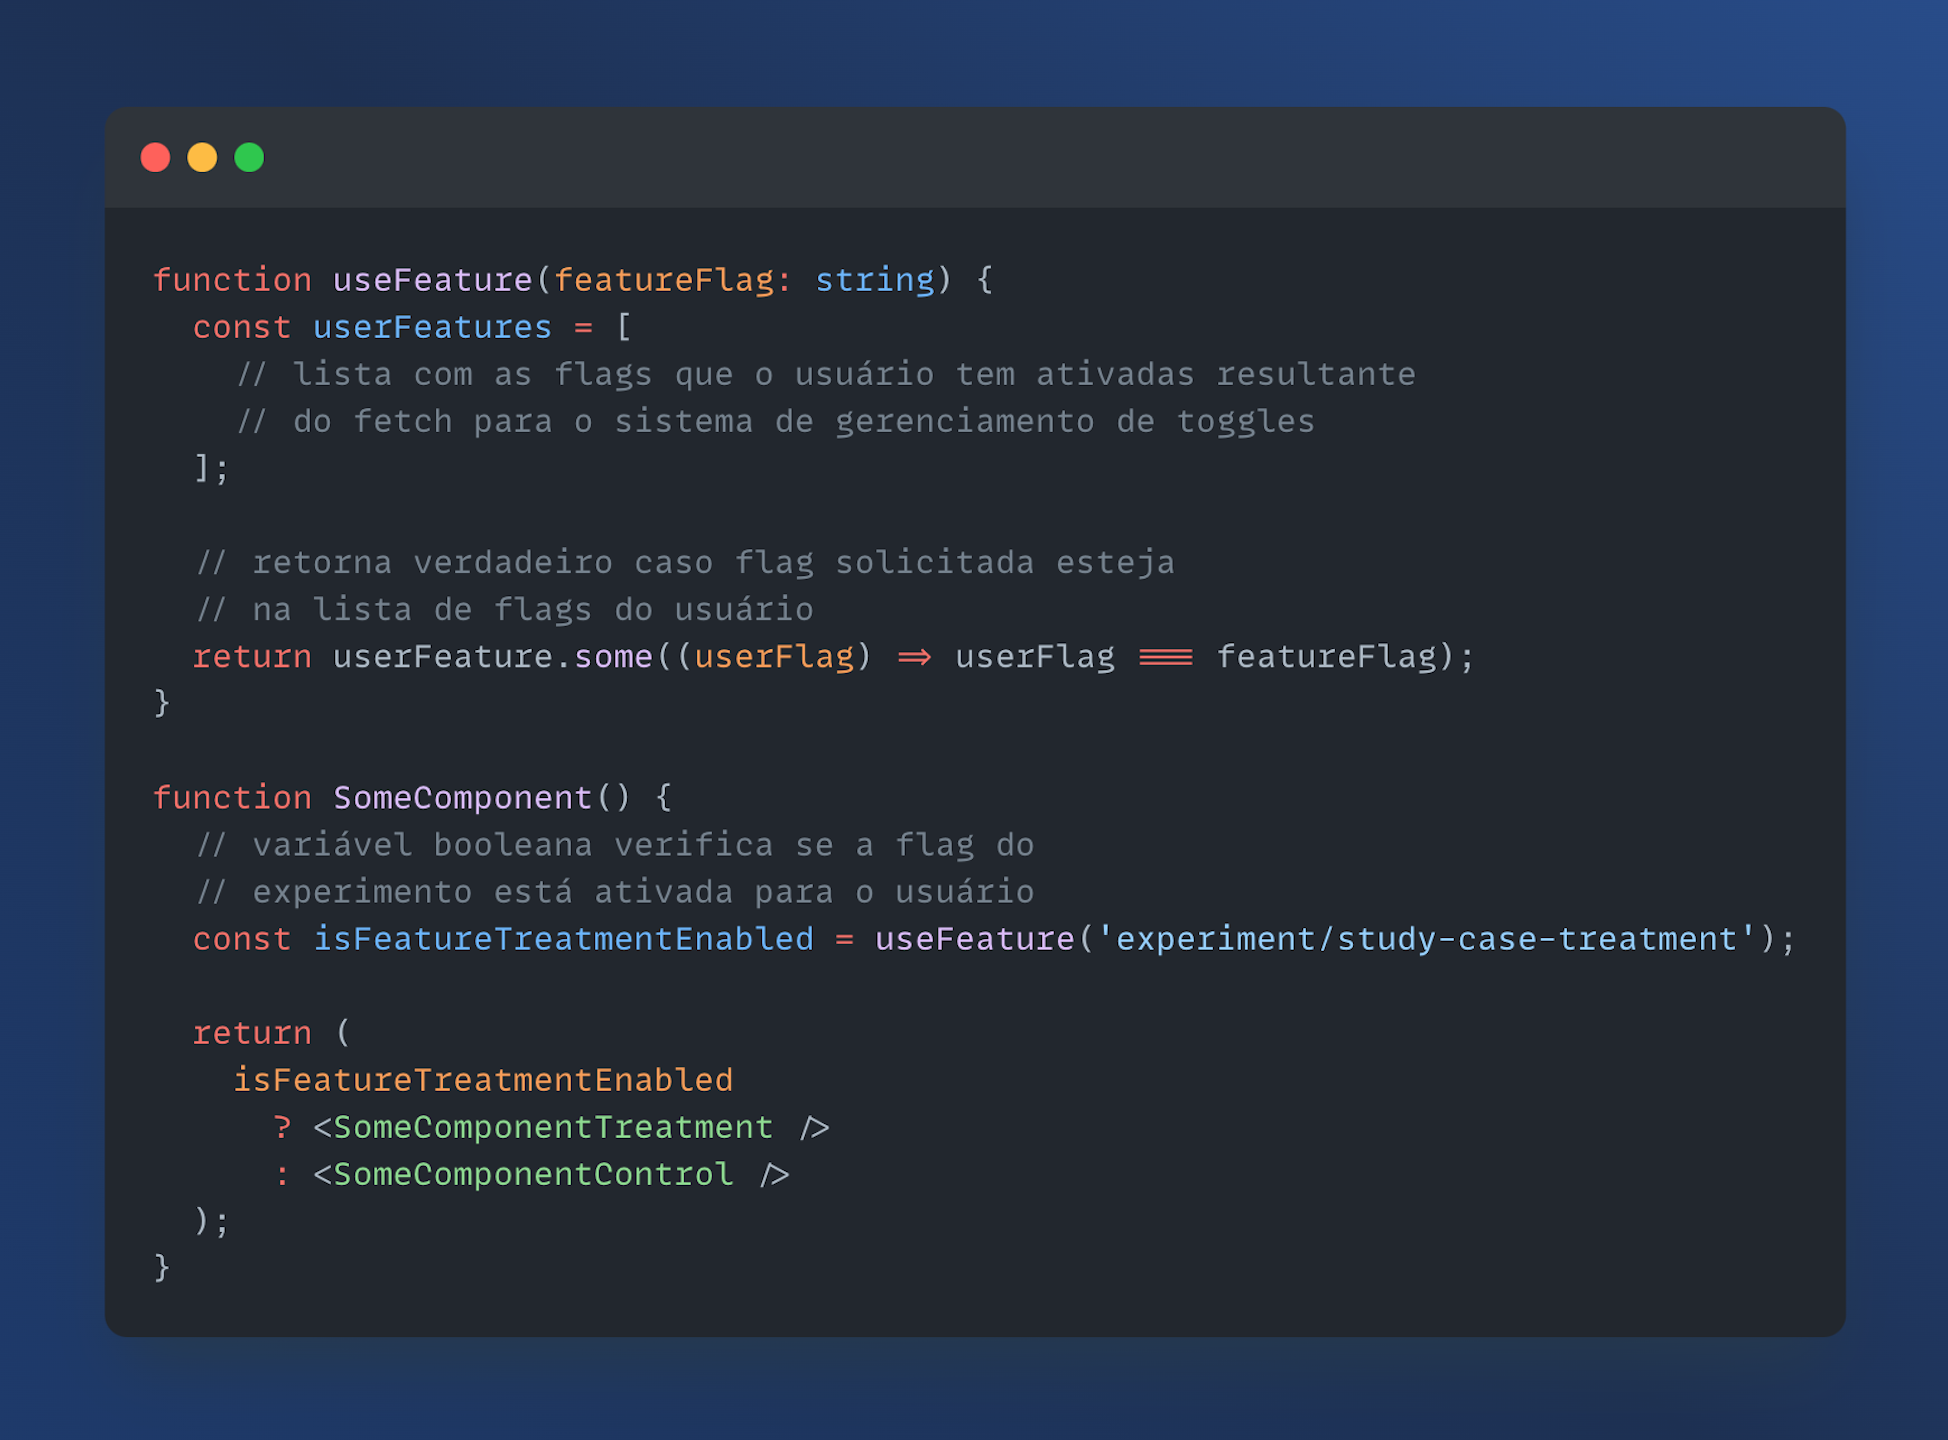
\includegraphics[width=1\linewidth]{figuras/toggle.png}
    \begin{center}
        \text{Fonte: Autor}
    \end{center}
    \label{fig:toggle}
\end{figure}

\section{Análise de Dados}


Antes de testes inferenciais, será realizada uma análise estatística descritiva das amostras, fundamental para compreender a natureza dos dados (Seção \ref{subsec:descritiva}). Esta etapa permite encontrar possívels \textit{outliers} (valores atípicos) e anomalias que possam enviesar os resultados. Esta análise oferece uma visão geral das tendências centrais e dispersão dos dados através de valores como a média, mediana, desvio padrão e distribuição do conjunto. Também serão utilizados métodos de representação gráfica, como \textit{boxplots} ou histogramas para análise da distribuição da amostra. Toda esta análise influência diretamente no teste estatístico adequado.

% Caso os dados coletados sejam contínuos (numéricos) e apresentem uma distribuição normal, o Teste T de Student (Seção \ref{subsec:t-test}) será utilizado para comparar as médias entre os dois grupos de dados (controle e tratamento). Este teste permite verificar se há uma diferença estatística significativa entre as métricas de uso de cada versão analisada. É uma abordagem eficiente para detectar diferenças entre grupos aproximadamente normais e com variâncias semelhantes.

% Por outro lado, caso as métricas escolhidas para análise sejam categóricas ou não sigam a distribuição normal, o Teste de Mann-Whitney U (Seção \ref{subsec:u-test}) será empregado. Este teste é uma alternativa ao T de Studente, pois é não paramétrico, ou seja, não parte do pressuposto de normalidade da amostra, sendo uma abordagem efetiva em casos de dados assimétricos. 

À depender das métricas escolhidas para análise e das características das amostras coletadas, será escolhido o teste de hipótese mais apropriado, conforme apresentado na Seção \ref{sec:ref-analise-dados}. A escolha destes tipos de teste se justifica dado o contexto do estudo de caso: serão comparadas apenas dois conjuntos de dados, e estas amostras são independentes, não havendo necessidade de testes que sirvam para cenários diferentes do descrito. 

Após essa análise quantitativa, com a finalização e documentação do experimento, serão coletados dados qualitativos referentes ao processo realizado, por meio de formulários de opinião com os colaboradores envolvidos. Esse levantamento buscará compreender, através das suas perspectivas, o desempenho e a aplicabilidade do procedimento executado, complementando a análise de dados quantitativos.


\section{Instrumentação}

Nesta seção, são apresentadas as ferramentas utilizadas na realização do estudo de caso. As soluções abordadas incluem o versionamento do código-fonte, a coleta de métricas de uso da plataforma, a análise de dados para testes de hipótese, a gestão e documentação das hipóteses geradas e a coleta de opiniões dos colaboradores envolvidos.

\subsection{Formulários Google}

O Google Forms é uma solução prática para a criação de questionários \textit{online} \cite{forms}. Além da formulação e organização das perguntas, a ferramenta permite gerenciar as respostas dos participantes, facilitando a análise dos resultados. Nesta monografia, a plataforma será utilizada para coletar informações sobre as opiniões dos colaboradores envolvidos no processo.

\subsection{Git e GitHub}

O Git é um sistema descentralizado d controle de versão que permite registrar as alterações realizadas nos arquivos de código de um \textit{software} ao longo do tempo, possibilitando o armazenamento de diferentes versões e a restauração de versões anteriores \cite{git}.

Já o GitHub é uma plataforma de desenvolvimento baseada no Git, que permite o armazenamento e compartilhamento de repositórios de código fonte, viabilizando a colaboração entre desenvolvedores \cite{github}. Como padrão no produto investigado, será utilizado para armazenar as versões de código analisadas neste estudo.

\subsection{Jupyter Notebook e JupyterHub}

O Jupyter Notebook é uma ferramenta de código aberto que permite o compartilhamento de documentos que podem conter, entre outros artefatos, arquivos de código para execução de \textit{scripts} \cite{jupyter_notebook}. Esses notebooks, através do processamento de código-fonte e linguagem \textit{markdown}, facilitam atividades colaborativas, como análise de dados e modelagem computacional.

No contexto desta pesquisa, notebooks serão utilizados para o tratamento dos dados, consumindo a API que fornece as métricas de uso da plataforma e permitindo a análise dos dados por meio de \textit{scripts} para o cálculo dos testes de hipótese apropriados.

O JupyterHub, que já é um padrão no produto investigado, é uma plataforma que permite o armazenamento e o compartilhamento de notebooks, será utilizada para o armazenamento do \textit{script} de análise de dados para realização de experimentos, viabilizando o acesso por parte de outros colaboradores da empresa \cite{jupyterhub}.

\subsection{MixPanel}

O MixPanel é uma plataforma de análise de engajamento que facilita o rastreamento e a compreensão do comportamento dos usuários em aplicações \textit{web} e \textit{mobile} \cite{mixpanel2024}. Esta plataforma será utilizada para instrumentalizar a coleta de métricas de comportamento em uso dos usuários, que serão utilizados nos testes de hipótese. Como já é utilizada no produto investigado, não será necessária a configuração da ferramenta adicional, apenas a definição dos eventos a serem observados durante o experimento.

A plataforma fornece bibliotecas que viabilizam o disparo de eventos diretamente no código-fonte do produto, e, além da coleta da métrica em si, também é possível adicionar propriedades específicas ao evento, como informações sobre o usuário, sobre seu comportamento, entre outras. Além disso, o MixPanel fornece uma API de consumo destes dados, permitindo ao desenvolvedor filtrá-los conforme necessário. Esta união de fatores permite que os dados além de computados, carreguem metadados que viabilizem filtragens e manipulações.

Na Figura \ref{fig:exemplo-mixpanel-cliente} é possível verificar o disparo do evento no lado do cliente, onde o mesmo carrega o nome do evento e os metadados necessários para manipulação e análise do mesmo. Já na Figura \ref{fig:exemplo-mixpanel-consumo} é apresentado um código em \textit{Python} com um exemplo do consumo da API da plataforma onde se solicitam os eventos disparados pelo exemplo da Figura \ref{fig:exemplo-mixpanel-cliente}. Desta forma é possível ver como se pretende instrumentalizar a coleta das métricas e também o consumo das mesmas para a realização da análise através da ferramenta MixPanel.

\begin{figure}
    \centering
    \caption{Exemplo de Disparo de Evento no MixPanel}
    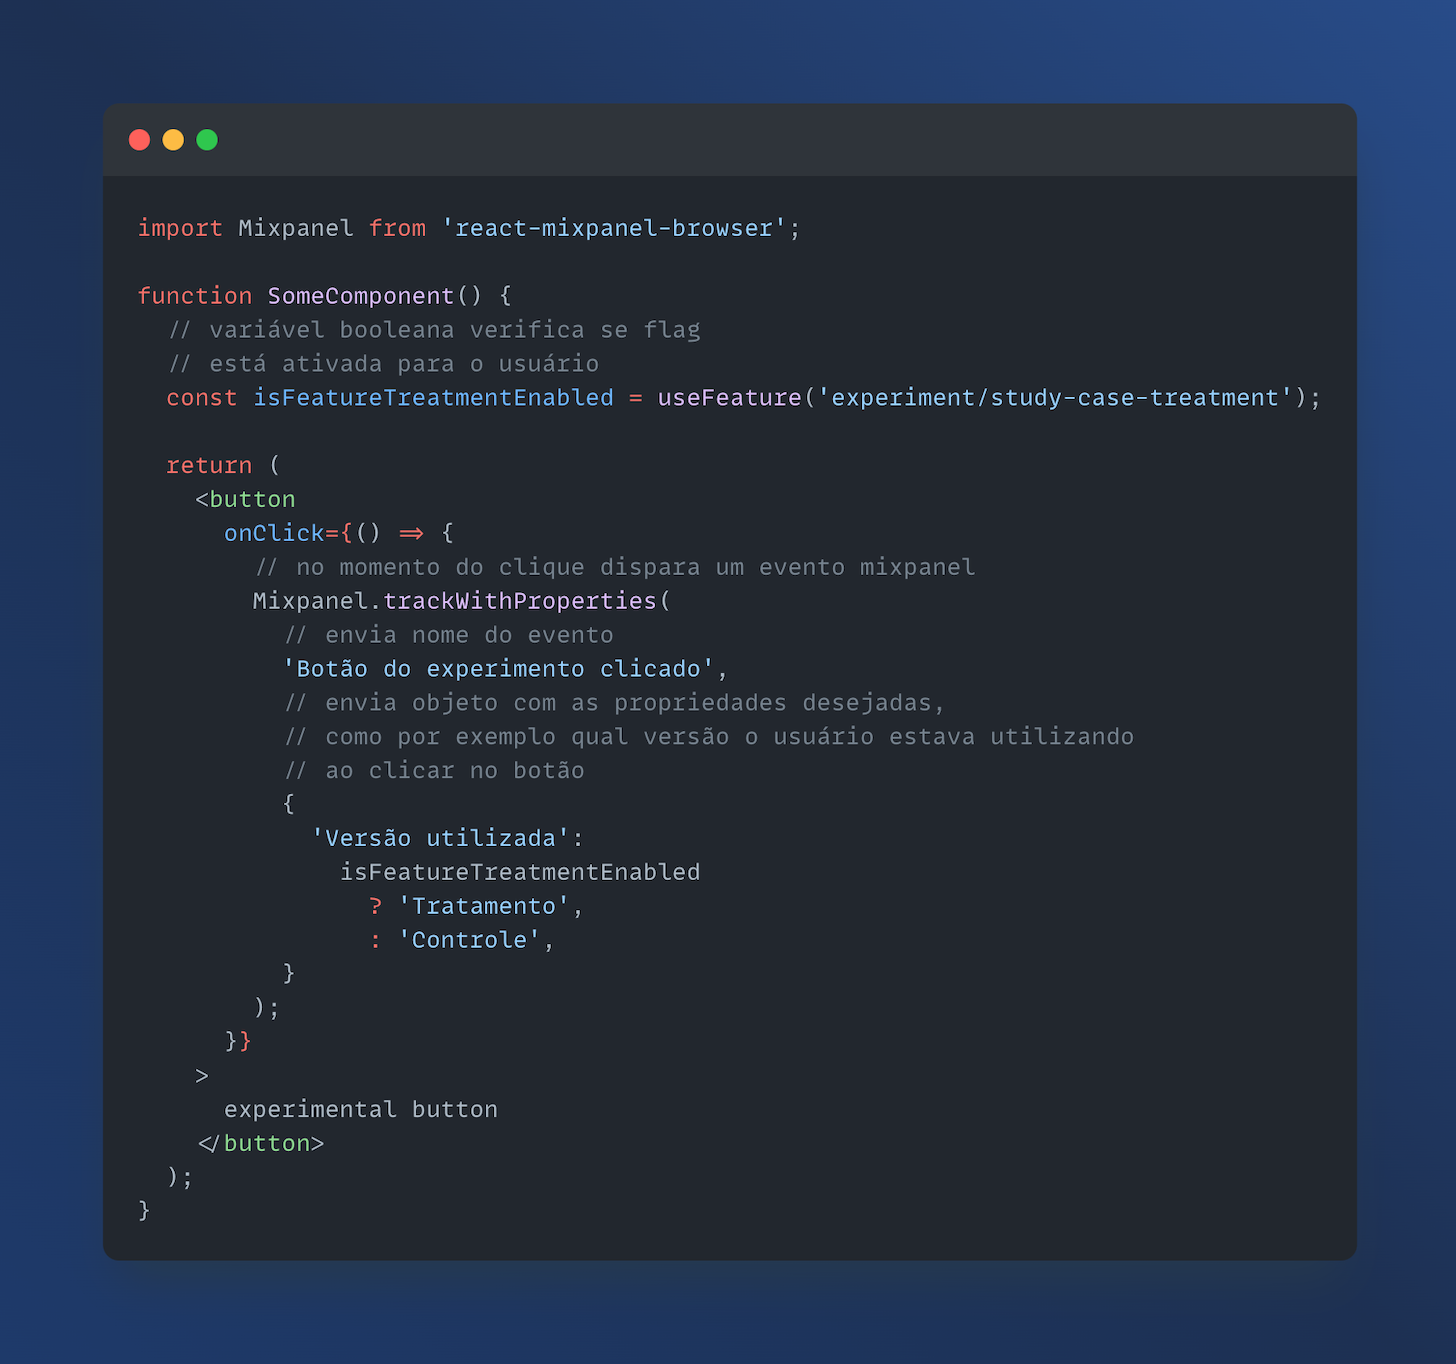
\includegraphics[width=0.75\linewidth]{figuras/exemplo_mixpanel.png}
    \begin{center}
        \text{Fonte: Autor}
    \end{center}
    \label{fig:exemplo-mixpanel-cliente}
\end{figure}

\begin{figure}
    \centering
    \caption{Exemplo de Consumo da API do MixPanel}
    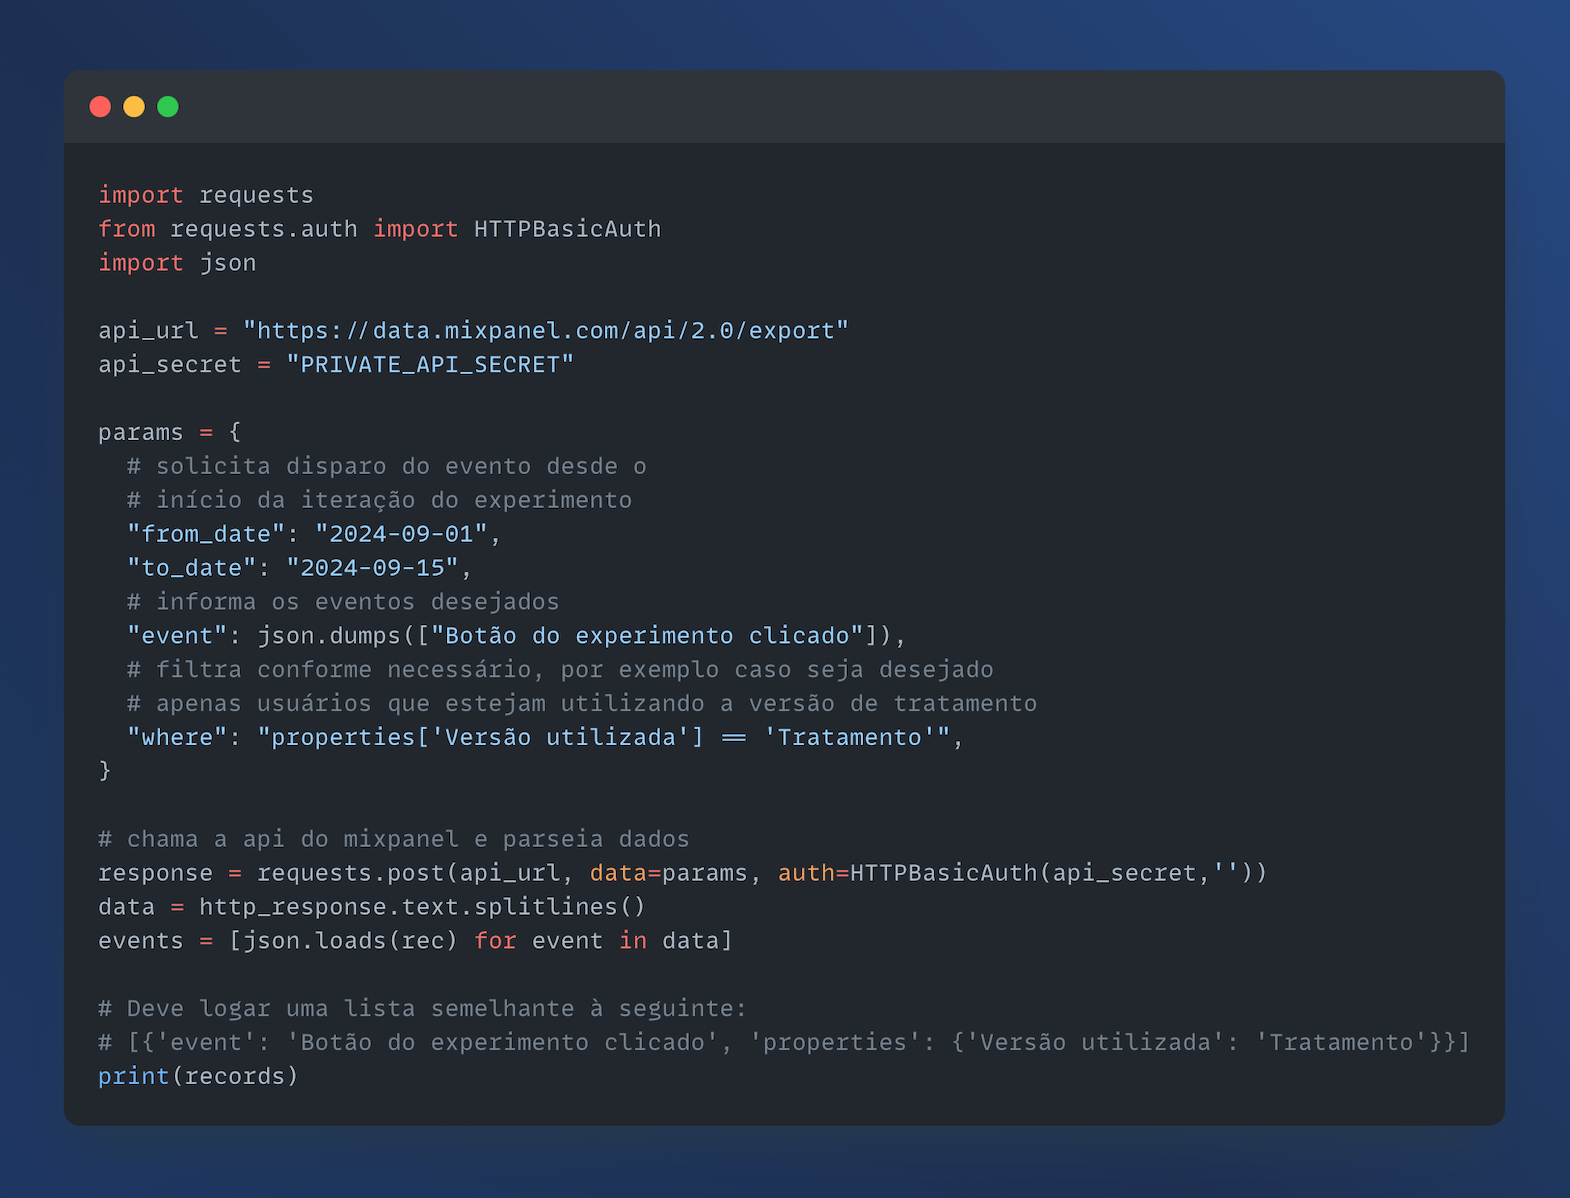
\includegraphics[width=0.75\linewidth]{figuras/exemplo_mixpanel_consumo.png}
    \begin{center}
        \text{Fonte: Autor}
    \end{center}
    \label{fig:exemplo-mixpanel-consumo}
\end{figure}

\subsection{Notion}

O Notion é uma plataforma multifuncional que combina funcionalidades de anotação, criação de documentos estruturados, dashboards personalizados, entre outras \cite{notion}. A ferramenta já é utilizada na empresa para centralizar documentações e dados, permitindo o acesso por todos os colaboradores.

Neste estudo de caso, o Notion será utilizado para documentar as hipóteses e experimentos, registrando os aprendizados. A plataforma servirá para gerenciar e armazenar as hipóteses geradas e priorizadas, assim como os resultados do experimento realizado na segunda etapa do trabalho. Além disso, será elaborado um guia para execução do experimento, a fim de colaborar com futuras experimentações.

\subsection{Python}

Python é uma linguagem de programação aberta conhecida por ser amigável, flexível e de fácil aprendizado \cite{python}. Por causa destas características, a linguagem conta com várias bibliotecas criadas pela comunidade. Dentre elas, diversas que possibilitam o uso de técnicas de estatística descritiva, bem como a realização de testes estatísticos.

No contexto deste trabalho, Python será utilizado para desenvolver \textit{scripts} que irão recuperar os eventos de uso da plataforma MixPanel conforme necessário, além de auxiliar as análises e testes estatísticos. A Figura \ref{fig:python} apresenta um exemplo onde a linguagem é utilizada para essas atividades.


\begin{figure}
    \centering
    \caption{Exemplo de Utilização do Python Para Análise de Dados}
    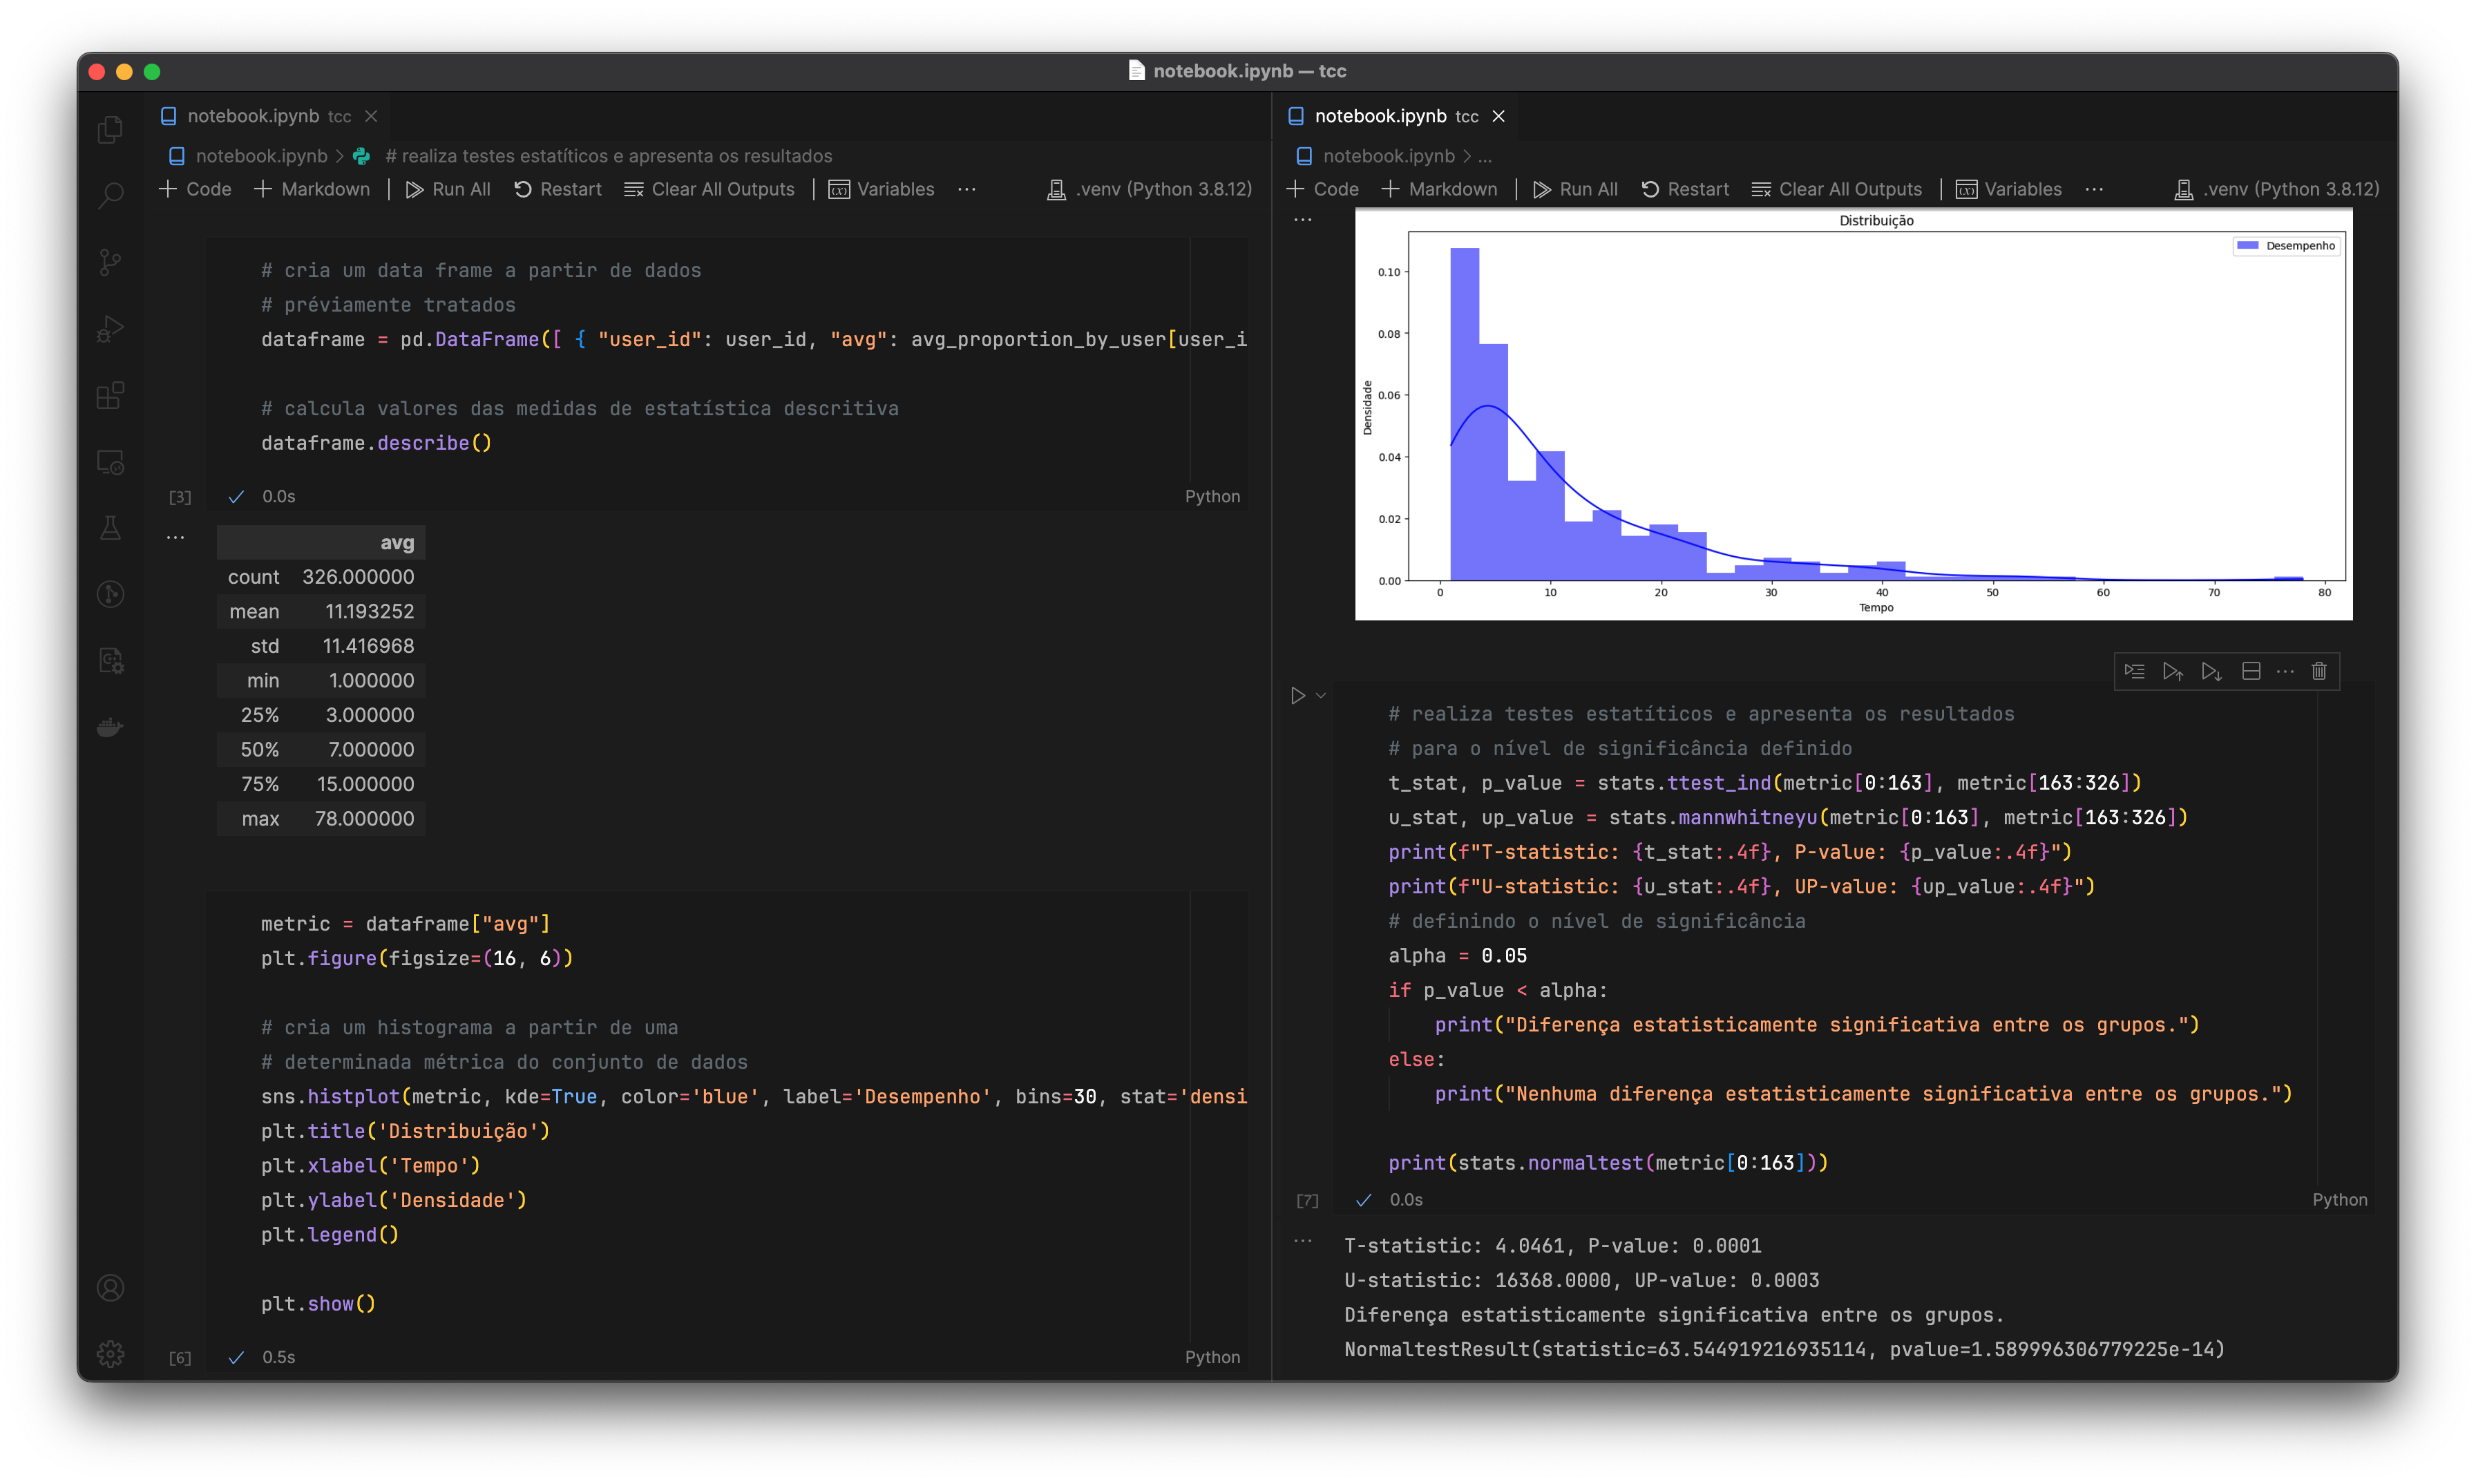
\includegraphics[width=1\linewidth]{figuras/python.png}
    \begin{center}
        \text{Fonte: Autor}
    \end{center}
    \label{fig:python}
\end{figure}


\chapter{Condições do Trabalho}
\label{ch:condicoes}

Neste capítulo é apresentada uma visão geral das atividades já realizadas e daquelas que ainda serão executadas na segunda etapa deste trabalho de conclusão de curso. Nele, são descritos os materiais já produzidos durante as tarefas concluídas, bem como um planejamento dos próximos passos.

\section{Atividades Concluídas}

Na Seção \ref{cronograma1}, foram descritas as atividades realizadas durante a primeira etapa desta pesquisa, com o objetivo de detalhar como os objetivos do trabalho seriam alcançados. A Tabela \ref{tab:atividades1} apresenta essas atividades, destacando o status atual de cada uma e os artefatos gerados por suas respectivas execuções.

\begin{table}[]
\centering
    \caption{Condição das Atividades da Primeira Etapa do Trabalho}
    \begin{tabular}{|p{8.5cm}|p{3cm}|p{3cm}|}
        \hline
        \textbf{Atividade} & \textbf{Condição} & \textbf{Resultados} \\ \hline
        Contextualização em Experimentação na Engenharia de Software & Concluída & Seção \ref{subsec:experimentacao} \\ \hline
        Contextualização em Experimentação Contínua & Concluída & Seções \ref{sec:ref-experimentacao-continua} e \ref{sec:ref-analise-dados} \\ \hline
        Definição dos Objetivos e Protocolo de Pesquisa & Concluída & Seções \ref{sec:rsl-protocolo} e \ref{subsec:objetivos-pesquisa} \\ \hline
        Execução da Busca e Seleção do Material & Concluída & Seção \ref{subsec:experimentacao} \\ \hline
        Leitura do Material Selecionado & Concluída & Seção \ref{sec:rsl-resultados} \\ \hline
        Definição da Proposta de Estudo de Caso & Concluída & Capítulo \ref{ch:proposta} \\ \hline
        Escrita da Monografia & Concluída & - \\ \hline
        Revisão da Monografia & Concluída & - \\ \hline
        Apresentação da Monografia & Agendada & - \\ \hline
    \end{tabular}

    \label{tab:atividades1}
    
    \begin{center}
        \text Fonte: Autor
    \end{center}
\end{table}


\section{Objetivos Específicos}

Os objetivos específicos elencados para esta pesquisa e apresentados na Seção \ref{subsec:objetivos-pesquisa} foram levantados visando guiar a execução deste trabalho em sua plenitude, tanto a primeira quanto a segunda etapa. A primeira etapa abrangeu a fundamentação teórica da pesquisa e a formulação da proposta de solução que será avaliada por meio de um estudo de caso. Já a segunda, visa a validação do processo proposto, realizando as atividades e documentando os resultados obtidos. Desta forma, na Tabela \ref{tab:objetivos-especificos}, é apresentada a condição atual dos objetivos específicos.


\begin{table}[]
\centering
    \caption{Condição dos Objetivos Específicos do Trabalho}
    \begin{tabular}{|p{8cm}|p{2cm}|p{4.5cm}|}
        \hline
        \textbf{Objetivo} & \textbf{Condição} & \textbf{Resultados} \\ \hline
        Levantamento Teórico & Atingido & Capítulo \ref{ch:referencial} \\ \hline
        Sistematizar Processo de Experimentação & Atingido & Seção \ref{sec:procedimentos} e Figura \ref{fig:processo-novo} \\ \hline
        Planejar Estudo de Caso & Atingido & Capítulo \ref{ch:proposta} \\ \hline
        Execução das Atividades Propostas & Pendente & - \\ \hline
        Coleta da Percepção dos Envolvidos & Pendente & - \\ \hline
        Analisar e Documentar os Resultados & Pendente & - \\ \hline
    \end{tabular}

    \label{tab:objetivos-especificos}
    
    \begin{center}
        \text Fonte: Autor
    \end{center}
\end{table}


\section{Próximos Passos}

Na segunda etapa, para a conclusão desta pesquisa, serão realizadas as atividades propostas no Capítulo \ref{ch:proposta}, em conjunto com os colaboradores participantes no desenvolvimento do produto sendo estudado. Finalizadas estas tarefas, os resultados obtidos serão analisados, documentados e apresentados. É planejado que esta execução siga o cronograma apresentado na Imagem \ref{fig:cronograma_2}.

\section{Resumo do Capítulo}

Este capítulo apresenta a condição atual das atividades deste trabalho, dos objetivos atingidos e pendentes e também as atividades a serem realizadas na próxima etapa. As Tabelas \ref{tab:atividades1} e \ref{tab:objetivos-especificos} explicitam as atividades e objetivos de acordo com sua condição e os artefatos resultados das etapas concluídas.
\bookmarksetup{startatroot} 

\postextual
%{bibliografia}
\justifying 
\bibliography{bibliography} %{<mybib>} 
% \bibliography{}

% \bibliographystyle {}
%\begin{anexosenv}
\partanexos

\end{anexosenv}


\input{editaveis/apendices}
\printindex
\end{document}

